\documentclass{beamer}
\usepackage{graphicx} % Required for inserting images
\usepackage{float}
\usepackage{hyperref}
\hypersetup{
    colorlinks=true,
    linkcolor=black,
    filecolor=magenta,      
    urlcolor=cyan,
    pdftitle={Overleaf Example},
    pdfpagemode=FullScreen,
    }
\usepackage{amsmath}
\usepackage{amsfonts}
\usepackage{amssymb}
\usepackage{dsfont}
\usepackage{adjustbox}
\usepackage{xcolor}
\usepackage{tcolorbox}
\usepackage{multirow}
\usetheme{Warsaw}
\usepackage{minted}
\usepackage[portuguese]{babel}
\usepackage{tcolorbox}
\tcbuselibrary{skins} 
% Definindo o contador
\newcounter{exerciciocontador}
\newcounter{definicaocontador}
\newcounter{exemplocontador}


\newtcolorbox{definicao}[1][]{
  enhanced,
  width=\textwidth, % Para ocupar toda a largura disponível
  colback=green!5!white,
  colframe=green!80!black,
  fonttitle=\bfseries\color{black}, % Título em preto
  title={Definição ~\refstepcounter{definicaocontador}\thedefinicaocontador: \quad },
  left=3mm,
  right=3mm,
  top=2mm,
  bottom=2mm,
  sharp corners,
  boxrule=0.9pt,
  drop shadow,
  attach title to upper,
  #1
}

\newtcolorbox{exercicio}[1][]{
  enhanced,
  width=\textwidth, % Para ocupar toda a largura disponível
  colback=red!5!white,
  colframe=red!80!black,
  fonttitle=\bfseries\color{black}, % Título em preto
  title={Exercício ~\refstepcounter{exerciciocontador}\theexerciciocontador: \quad },
  left=3mm,
  right=3mm,
  top=2mm,
  bottom=2mm,
  sharp corners,
  boxrule=0.9pt,
  drop shadow,
  attach title to upper,
  #1
}
\newtcolorbox{atencao}[1][]{
  enhanced,
  width=\textwidth, % Para ocupar toda a largura disponível
  colback=red!5!white,
  colframe=red!70!black,
  fonttitle=\bfseries\color{black}, % Título em preto
  title={Atenção: \quad },
  left=3mm,
  right=3mm,
  top=2mm,
  bottom=2mm,
  sharp corners,
  boxrule=0.9pt,
  drop shadow,
  attach title to upper,
  #1
}

\newtcolorbox{exemplo}[1][]{
  enhanced,
  width=\textwidth, % Para ocupar toda a largura disponível
  colback=red!2!white,
  colframe=red!40!black,
  fonttitle=\bfseries\color{black}, % Título em preto
  title={Exemplo ~\refstepcounter{exemplocontador}\theexemplocontador: \quad },
  left=3mm,
  right=3mm,
  top=2mm,
  bottom=2mm,
  sharp corners,
  boxrule=0.9pt,
  drop shadow,
  attach title to upper,
  #1
}


\AtBeginSection[]{
  \begin{frame}
  \vfill
  \centering
  \begin{beamercolorbox}[sep=8pt,center,shadow=true,rounded=true]{title}
    \usebeamerfont{title}\insertsectionhead\par%
  \end{beamercolorbox}
  \vfill
  \end{frame}
}


\title{Estatística para Administração}
\author{ Prof. Ismael Bastos}
\date{}

\begin{document}

\begin{frame}
    \titlepage
    \begin{figure}[htpb]
        \begin{center}
            
\includegraphics[width=0.25\linewidth]{figures/arbalest.png}
        \end{center}
    \end{figure}
\end{frame}

\section{Introdução à Estatística e Informações da Disciplina}
\begin{frame}{O que é Estatística}
    Entendemos a Estatística como um conjunto de técnicas que permite, de forma sistemática,
organizar, descrever, analisar e interpretar dados oriundos de estudos ou
experimentos, realizados em qualquer área do conhecimento. 
\end{frame}

\begin{frame}{Áreas da Estatística}

Podemos dividir a Estatística em três áreas:
\begin{itemize}
    \item Estatística Descritiva
    \item Probabilidade
    \item Inferência Estatística
\end{itemize}
    
\end{frame}

\begin{frame}{Áreas da Estatística}
\begin{itemize}
    \item \textbf{Estatística Descritiva} (\textit{Conheça seus dados}) : Etapa inicial em qualquer análise de dados. É um conjunto de métodos estatísticos que tem por objetivo a organização, descrição e o resumo de dados. 
\pause 
    \item \textbf{Probabilidade} (\textit{Qual a incerteza associada aos dados?}) : Auxilia na modelagem de fenômenos aleatórios, ou seja, aqueles em que há incerteza.
\pause
    \item \textbf{Inferência Estatística} (\textit{Quais conclusões podemos tirar a partir destes dados?}): É um método estatístico que possibilita tirar conclusões sobre uma população a partir de informações contidas na amostra.
\end{itemize}

\end{frame}
\begin{frame}{População x Amostra}

\begin{figure}
    \centering
    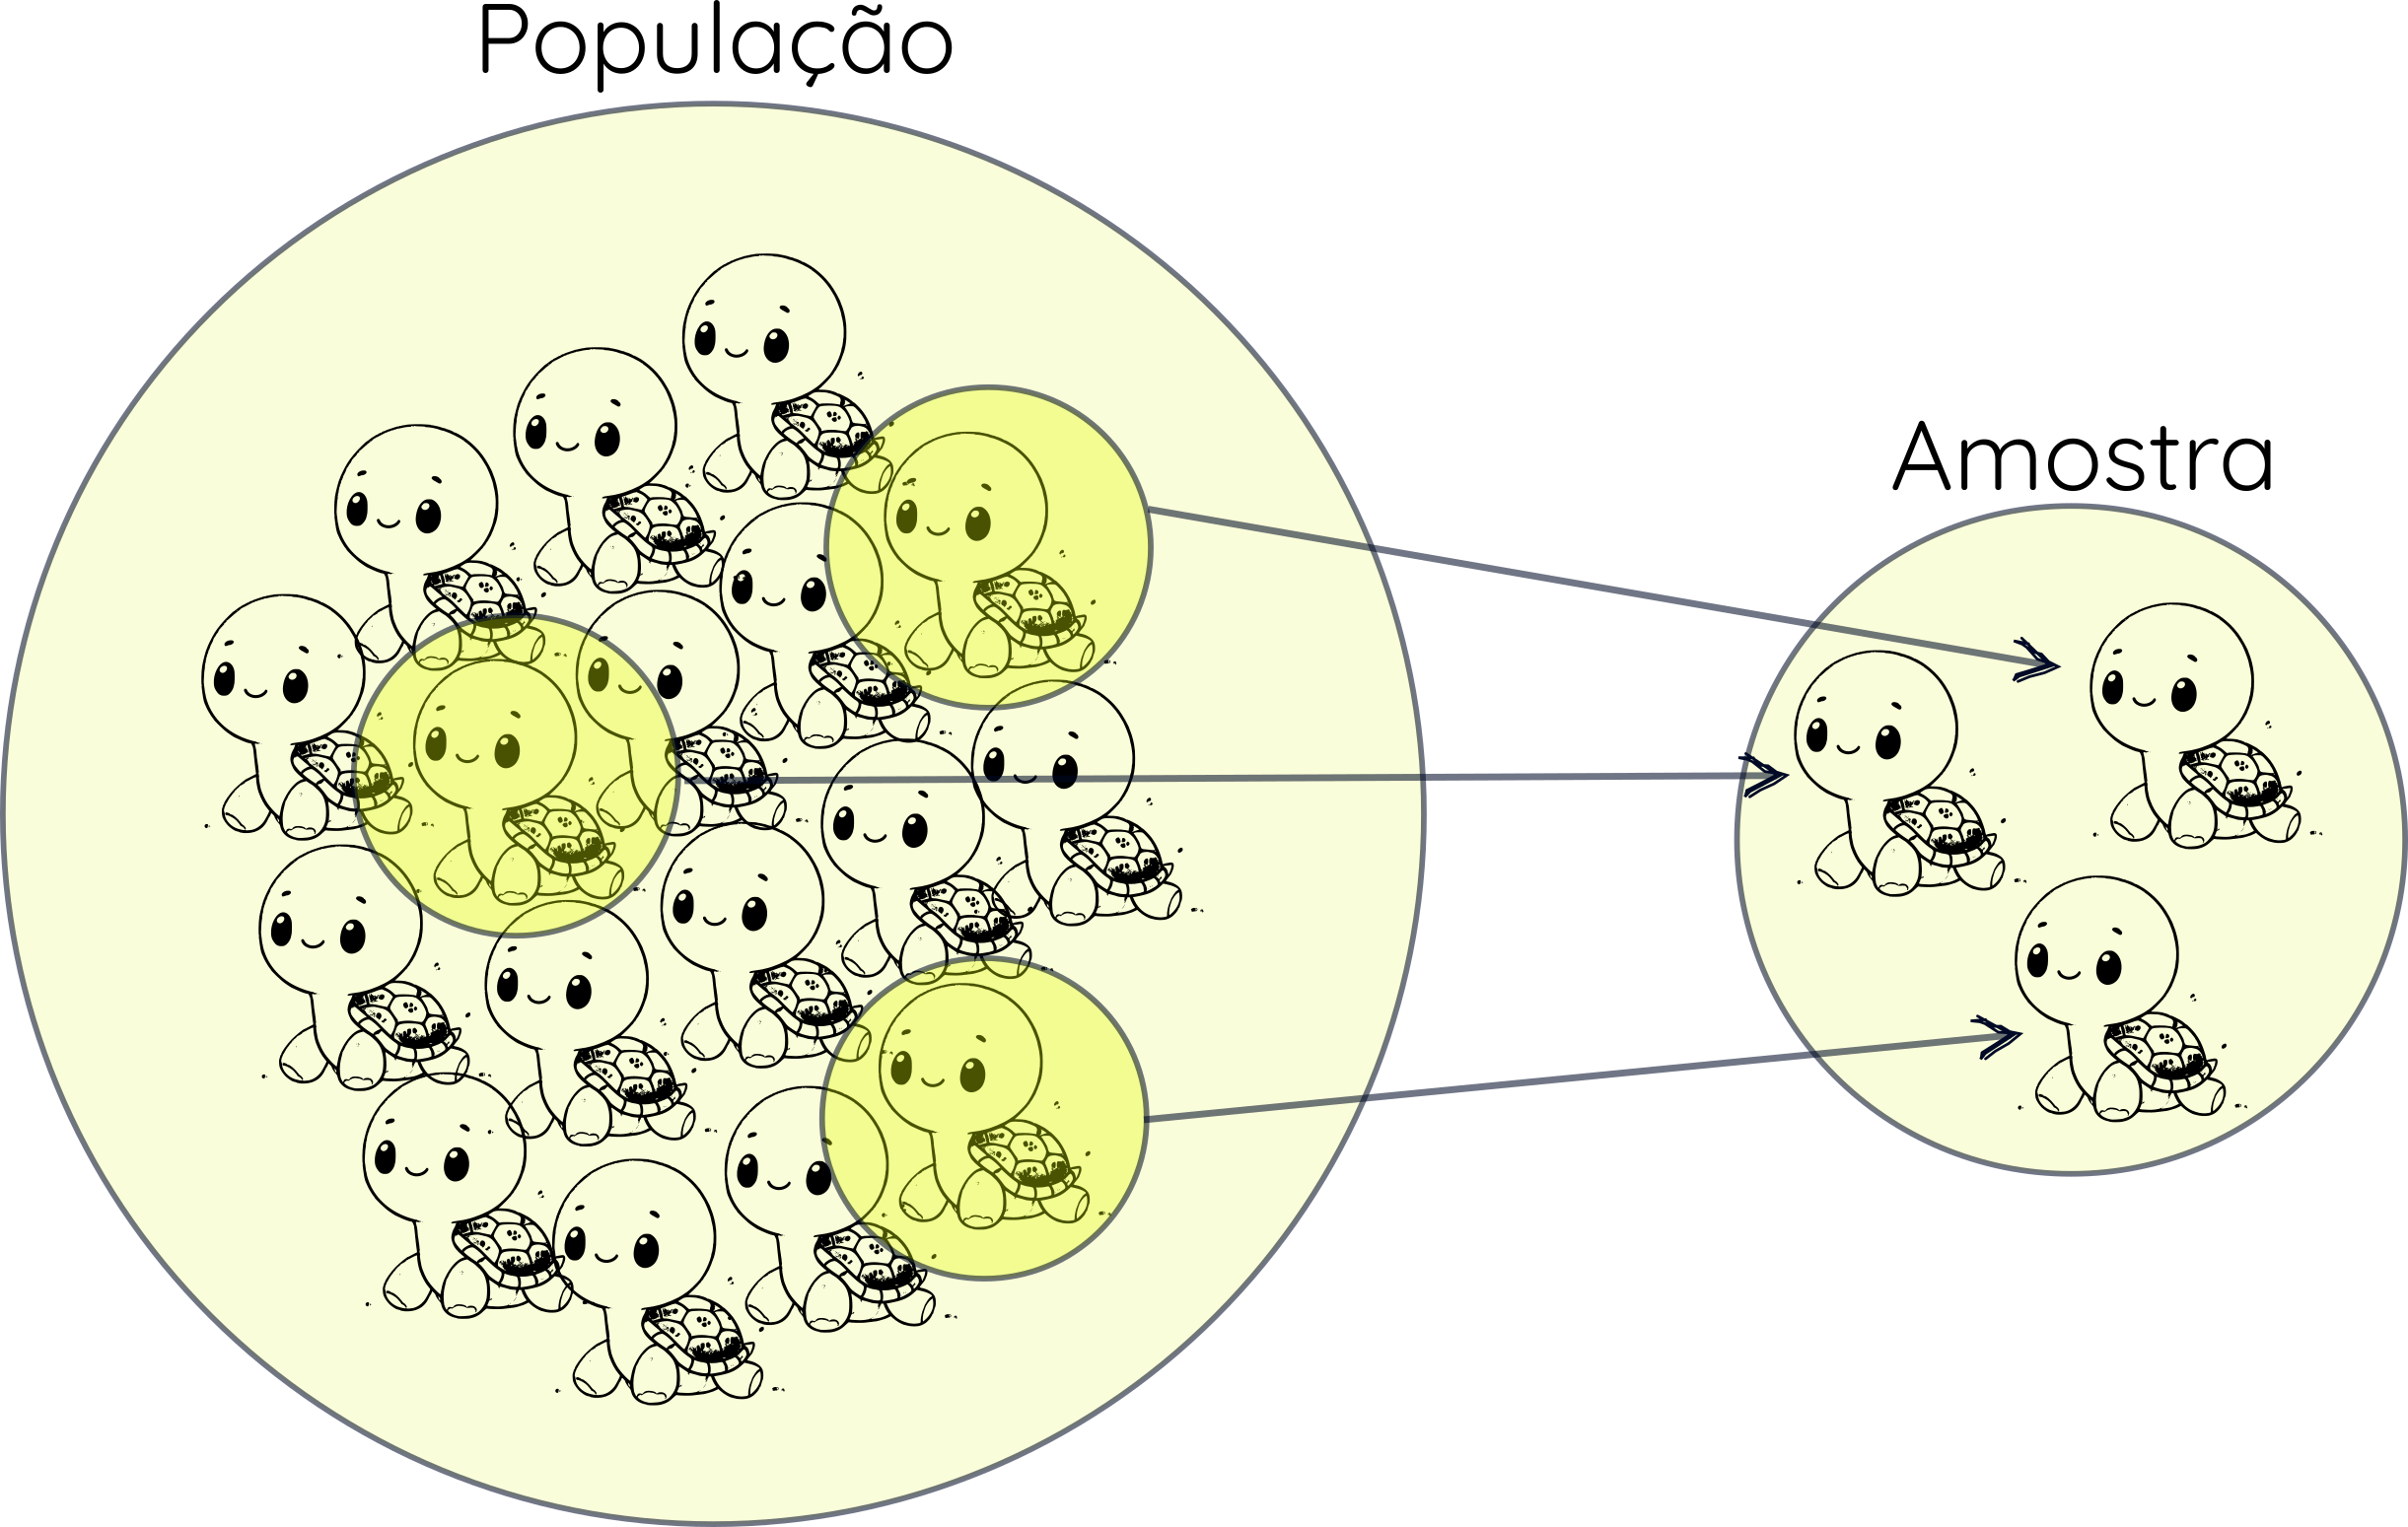
\includegraphics[width=0.7\linewidth]{figures/pop_sample.png}
\end{figure}
\end{frame}

\begin{frame}{População x Amostra}
    Por que precisamos selecionar uma amostra?
\end{frame}
\begin{frame}{Áreas da Estatística}
    \begin{figure}
        \centering
        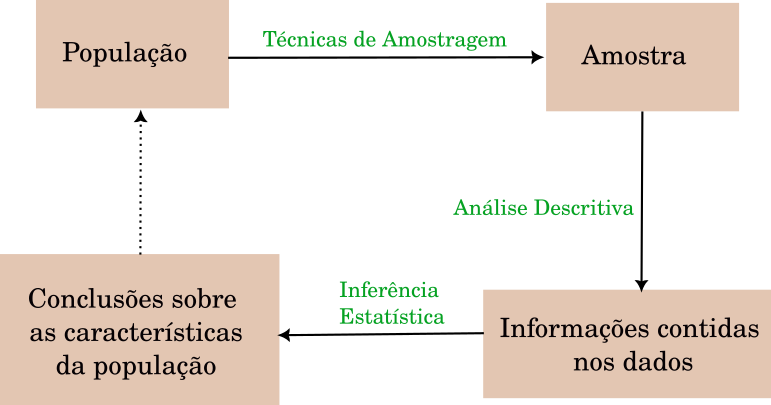
\includegraphics[width=0.8\linewidth]{figures/int_1.png}
    \end{figure}
\end{frame}

\begin{frame}{Informações da Disciplina}
\begin{itemize}
    \item Trabalho 1 valendo 10 pontos 
    \item Prova 1 valendo 10 pontos 
    \item Prova 2 valendo 10 pontos 
\end{itemize}


$$\text{Nota Final} = 0,4 \cdot T_1 + 0,3 \cdot P_1 + 0,3 \cdot P_2$$

\end{frame}
\begin{frame}{Funcionamento da disciplina}
    \begin{itemize}
        \item Aulas expositivas com conteúdo em slide. 
        \item Aulas práticas envolvendo aplicações. 
        \item Resolução de exemplos e exercícios no quadro *.
        \item Uso da linguagem de programação R.
        \item Disponibilização de informações da disciplina através do site da disciplina e do SIGA. 
        \item Listas de exercício
        \item Alguns códigos estarão presentes nos slides, mas alguns outros serão disponibilizados separadamente.
    \end{itemize}
    *: A resolução de exemplos e exercícios não será disponibilizada no site.
\end{frame}

\begin{frame}{Linguagem de programação R}
    \begin{itemize}
        \item Por que usar a linguagem R para estatística?
        \item Instalação do R e R Studio. 
        \item Posit Cloud. 
    \end{itemize}
\end{frame}


\subsection{Conceitos iniciais: Amostragem}
\begin{frame}{Perguntas iniciais}
\begin{itemize}
    \item Como garantir que uma amostra representa bem a população?
    \begin{itemize}
        \item Qual metodologia devo utilizar para selecionar minha amostra?
        
        \textbf{Exemplo}: Quero conduzir uma pesquisa eleitoral na cidade de São Paulo, como devo escolher as pessoas que vou entrevistar?
        \pause
        \item Qual tamanho de amostra selecionar?
        
        \textbf{Exemplo}: Sei que o tamanho da população de São Paulo é de aproximadamente $11,45$ milhões de habitantes, quantas pessoas devo escolher? 
    \end{itemize}
\end{itemize}
\end{frame}

\section{Amostragem}

\begin{frame}{Amostragem aleatória simples}
    \textbf{Amostragem aleatória simples:} Consideremos uma população de tamanho $N$ e desejamos uma amostra de tamanho $n$.
    A amostragem aleatória simples é feita da seguinte forma:
    \begin{enumerate}
        \item Numeramos os itens da população com número de $1$ até $N$.
        \pause
        \item Escrevemos cada um desses números em uma pedaço de papel.
        \pause
        \item Colocamos esses papeis em uma urna bem misturados.
        \pause
        \item Tiramos os $n$ papeis correspondentes à amostra. 
    \end{enumerate}
         \pause
\textbf{Pergunta}: \textcolor{red}{Essa retirada é com ou sem reposição?}   
\end{frame}

\begin{frame}{Amostragem aleatória simples - Exemplo}
\begin{exemplo}
    O estudo \href{https://www.scielo.br/j/inter/a/FH3ZBH3kPbKxDKrjwBgFHQD/}{O perfil socioeconômico e a percepção ambiental dos pescadores da Lagoa de Apodi,
     Rio Grande do Norte, Brasil} propõe uma amostragem aleatória simples como metodologia de amostragem. 
\end{exemplo}

    
\end{frame}
\begin{frame}[fragile]
\frametitle{Amostragem aleatória simples - Exemplo no R}
Nesse exemplo do R estamos assumindo que temos uma população de $10$ indivíduos cujos nomes estão armazenadas no vetor \textit{populacao} e desejamos
obter uma amostra de tamanho $3$ utilizando a amostragem aleatória simples. 
\begin{block}{Amostragem aleatória simples no R}
\begin{minted}[linenos=false,breaklines]{R}
n = 3
populacao = c("Tom", "Lia", "Ema", "Max", "Ana", "Lua", "Mia", "Isa", "Ilo", "Gal")
amostra = sample(populacao, n)
\end{minted}
\end{block}
\pause
A função \textit{sample} gera uma amostra aleatória simples de tamanho $n$, que nesse caso é $3$.
\pause

\textcolor{red}{Observação:} A função \textit{sample} por padrão gera uma amostra selecionada sem reposição, para gerar uma amostra com reposição, basta 
adicionar o argumento \textit{replace = TRUE}.
\end{frame}

\begin{frame}{Amostragem aleatória estratificada}
\textbf{Amostragem aleatória estratificada: }Consideremos que temos uma população (\textcolor{red}{heterogênea}) de tamanho $N$ e desejamos uma amostra de tamanho $n$.
A amostragem aleatória estratificada é feita da seguinte forma:
\begin{enumerate}
    \item Dividimos a população em estratos (com base em Idade, Renda, Sexo, Escolaridade ou outra variável).
    \pause
    \item Determinamos o tamanho da amostra que iremos retirar de cada estrato, podendo ser feito de duas principais formas:
    \pause
    \begin{itemize}
        \item \textbf{Proporcional}: A quantidade de indivíduos amostrados em cada estrato é proporcional ao tamanho do estrato. 
        \item \textbf{Igualitária}:  Selecionamos o mesmo número de indivíduos em cada estrato, não levando em conta o tamanho. 
    \end{itemize}
    \pause
    \item Realizamos a amostragem aleatória simples em cada estrato. 
\end{enumerate}
\end{frame}

\begin{frame}{Amostragem aleatória estratificada - Exemplo}
    \begin{exemplo}
    O estudo \href{https://www.scielo.br/j/rbso/a/bMg5nzYYqSBGWCjZrzjhYPb/}{Hipertensão Arterial e Diabetes Mellitus entre trabalhadores da saúde: associação com hábitos de vida
    e estressores ocupacionais} propõe uma amostragem aleatória estratificada como metodologia de amostragem.     
    \end{exemplo}
   
\end{frame}

\begin{frame}[fragile]
\frametitle{Amostragem aleatória estratificada - Exemplo no R}
\begin{block}{Amostragem aleatória estratificada (Proporcional) no R}
\begin{minted}[linenos=false,breaklines]{R}
n = 3
populacao = c("Tom", "Lia", "Ema", "Max", "Ana", "Lua", "Mia", "Isa", "Ilo", "Gal")
populacao_M = c("Tom", "Max", "Ilo")
populacao_F = c("Lia", "Ema", "Ana", "Lua", "Mia", "Isa", "Gal")
amostra_1 = sample(populacao_M, round(0.3 * n))
amostra_2 = sample(populacao_F, round(0.7 * n))
amostra = c(amostra_1, amostra_2)
\end{minted}
\end{block}
\end{frame}

\begin{frame}{Amostragem aleatória estratificada}
\textbf{Amostragem aleatória estratificada em duas etapas:} Consideremos que temos uma população de tamanho $N$ e desejamos uma amostra de tamanho $n$.
A amostragem aleatória estratificada em duas etapas é feita da seguinte forma:
\begin{enumerate}
    \item Dividimos a população em estratos (com base em Idade, Renda, Sexo, Escolaridade ou outra variável).
    \pause
    \item Selecionamos aleatoriamente subconjuntos desses estratos.  
    \pause
    \item Realizamos amostragem aleatória simples dentro de cada grupo.
\end{enumerate}
\pause
\textcolor{red}{Atenção:} O número de etapas não está necessariamente relacionado ao número de variáveis.
\end{frame}
% \begin{frame}{Amostragem aleatória por conglomerados}
% \textbf{Amostragem aleatória por conglomerados: }Consideremos que temos uma população de tamanho $N$ e desejamos uma amostra de tamanho $n$.
% A amostragem aleatória por conglomerados é feita da seguinte forma:
% \begin{enumerate}
%     \item Dividimos a população em conglomerados (como, por exemplo, escolas, unidades de saúde, bairros, etc.).
%     \pause
%     \item Selecionamos aleatoriamente um subconjunto desses conglomerados.  
%     \pause
%     \item Todos os indivíduos dentro dos conglomerados selecionados são estudados
% \end{enumerate}
% \end{frame}

% \begin{frame}{Amostragem aleatória por conglomerados}
%     Como garantir que ao final teremos os $n$ indivíduos que desejávamos?

%     \pause

%     \textbf{Amostragem aleatória por conglomerados em duas etapas: }
%     \begin{enumerate}
%         \item Realizamos a amostragem aleatória por conglomerados conforme descrita no slide anterior. 
%         \item Definimos o tamanho da amostra retirada de cada conglomerado, podendo ser feito de duas formas:
%         \begin{itemize}
%             \item \textbf{Proporcional}: A quantidade de indivíduos amostrados em cada conglomerado é proporcional ao tamanho do estrato. 
%             \item \textbf{Igualitário}:  Selecionamos o mesmo número de indivíduos em cada conglomerado, não levando em conta o tamanho. 
%         \end{itemize}
%         \item Realizamos a amostragem aleatória simples em cada conglomerado. 
%     \end{enumerate}
% \end{frame}
% \begin{frame}{Amostragem aleatória por conglomerados X Amostragem aleatória estratificada}
%     \textcolor{red}{Importante:} Não confundir amostragem aleatória por conglomerados com amostragem aleatória estratificada.
%     \begin{table}[H]
%     \centering
%     \begin{adjustbox}{width=\textwidth}
%     \begin{tabular}{|c|c|}
%     \hline
%     \textbf{Amostragem aleatória por conglomerados} & \textbf{Amostragem aleatória estratificada} \\\hline
%     Grupos (Conglomerados) heterogêneos em seu interior & Grupos (Estratos) homogêneos em seu interior \\ \hline
%     Grupos (Conglomerados) homogêneos entre si & Grupos (Estratos) heterogêneos entre si \\ \hline
%     \end{tabular}
%     \end{adjustbox}
%     \end{table}
% \end{frame}

%     \begin{frame}{Amostragem aleatória sistemática}
%         \textbf{Amostragem aleatória sistemática: }Consideremos que temos uma população de tamanho $N$ e desejamos uma amostra de tamanho $n$.
%         A amostragem aleatória sistemática é feita da seguinte forma:
%         \begin{enumerate}
%             \item Determinamos o intervalo de amostragem $k = \dfrac{N}{n}$.
%             \pause
%             \item Selecionamos aleatoriamente um número entre $1$ e $k$ como ponto de partida. 
%             \pause
%             \item Selecionamos os elementos da amostra a partir do ponto de partida, seguindo o intervalo $k$.
%         \end{enumerate}
%         \pause 
%         \textcolor{red}{Perguntas:}
%         \begin{enumerate}
%             \item  No passo 1, precisamos de fato definir $k$ dessa forma? Em qual situação que poderíamos defini-lo de outra forma?
%             \pause
%             \item Qual o principal possível problema dessa abordagem?
%         \end{enumerate}
       
%         \pause

% \end{frame}

% \begin{frame}{Amostragem aleatória por conglomerados e sistemática - Exemplo}
%     \begin{exemplo}
%          O estudo \href{https://www.scielo.br/j/rbgg/a/PtkLqMxhrj8b7tQwBVgnr8z/abstract/?lang=pt}{Associação da depressão com as características sociodemográficas, qualidade do sono e hábitos de vida em idosos do Nordeste brasileiro: estudo seccional de base populacional.} 
%     propõe uma amostragem aleatória por conglomerados seguido pela amostragem aleatória sistemática como metodologia de amostragem.
%     \end{exemplo}
   
% \end{frame}

% \begin{frame}[fragile] 
% \frametitle{Amostragem aleatória sistemática - Exemplo no R}
% \begin{block}{Amostragem aleatória sistemática no R}
% \begin{minted}[linenos=false,breaklines]{R}
%     populacao = c("Tom", "Lia", "Ema", "Max", "Ana", "Lua", "Mia", "Isa", "Ilo", "Gal")
%     N = length(populacao)
%     n = 5
%     k = N/n
%     amostra = c()
%     valor_inicial = sample(seq(1,k), 1)
%     for(i in seq(valor_inicial,N, k)){
%       amostra = c(amostra, populacao[i])
%     }    
% \end{minted}
% \end{block}
% \end{frame}  

% \begin{frame}{Amostragem aleatória sistemática - Exemplo no R}
%     O código so slide anterior realiza a amostragem aleatória sistemática em um cenário
%     em que se deseja obter uma amostra de tamanho 5.
% \end{frame}

% \begin{frame}{Outros tipos de amostragem}
%  Considere, agora, que um aluno esteja interessado em avaliar a opinião dos alunos da UFRJ
% sobre o serviço de transporte entre os diversos campi, oferecido pela administração da universidade.  
% Como ele não tem \textbf{condições} nem \textbf{tempo} de selecionar uma amostra de todos
% os alunos a UFRJ, decide entrevistar seus colegas de turma.
% \pause
% \begin{itemize}
%     \item A decisão desse aluno é razoável? Ou seja, essa amostra é representativa?
%     \item Qual a diferença desse método para os que estudamos anteriormente?
% \end{itemize}
% \pause
% Esse tipo de amostragem é chamado de \textbf{amostragem por conveniência} e é um tipo de amostragem não-probabilística. 
% \end{frame}

% \begin{frame}{Outros tipos de amostragem}
%     Os métodos de amostragem não-probabilísticos são ruins e não devem ser utilizados???
% \end{frame}

% \begin{frame}{Problemas dos métodos de amostragem probabilísticos discutidos}
%     \begin{itemize}
%         \item Como vou ter acesso a lista de todas as pessoas da população?
%         \pause
%         \item Será que a informação sobre a proporção de elementos em cada estrato é confiável?
%     \end{itemize}
% \end{frame}

% \begin{frame}{O problema do viés - Experimento de aprisionamento de Stanford (1971)}
%     \begin{figure}
%         \centering
%         
\includegraphics[width=0.4\linewidth]{figures/filme_1.jpg}
%     \end{figure}
% \end{frame}

% \begin{frame}{O problema do viés - Experimento de aprisionamento de Stanford (1971)}
% \begin{itemize}
%     \item Participantes de uma comunidade local foram convidados através de um anúncio de jornal que recrutava estudantes do sexo masculino
%     para participar de um "\textbf{estudo psicológico da vida em uma prisão}". 
%     \pause
%     \item Caso o estudante fosse aprovado, receberia \$15 por dia (equivalente a aproximadamente \$120 atualmente).
%     \pause
%     \item Os participantes foram submetidos a testes psicológicos e alocados aleatoriamente na posição de prisioneiro ou carcereiro. 
%     \item \textbf{Conclusão do Experimento}: Pessoas "boas" podem ter um "mal" comportamento quando colocadas em posições de poder ou sob condições de estresse.  
% \end{itemize}
% \end{frame}

% \section{Análise Exploratória de Dados}

% \begin{frame}{Tipos de variáveis}
% \begin{itemize}
%     \item \textbf{Variável:} Característica analisada (Nome da coluna)
%     \begin{itemize}
%         \item \textbf{Quantitativa:} Assume valores numéricos 
%         \begin{itemize}
%             \item Discreta: Assume valores discretos, valores inteiros.
%             \item Contínua: Assume valores no intervalo dos números reais.
%         \end{itemize}
%         \item \textbf{Qualitativa:} Assume valores que representam atributos e/ou qualidades 
%         \begin{itemize}
%             \item \textbf{Ordinal}: Valores assumem ordem, indicando intensidade crescentes de realização
%             \item \textbf{Nominal}: Valores não assumem ordem 
%         \end{itemize}
%     \end{itemize}
% \end{itemize}
% \end{frame}

% \begin{frame}{Tipos de variáveis}
%     \begin{figure}
%         \centering
%         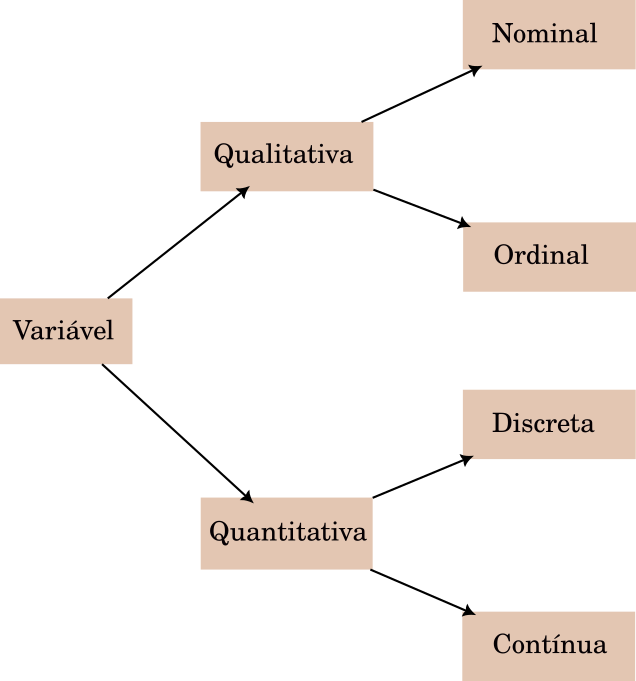
\includegraphics[width=0.5\linewidth]{figures/classificacao_variaveis.png}
%     \end{figure}
% \end{frame}

% \begin{frame}{Tipos de variáveis}
%     \textbf{Exemplo inicial }
%     \begin{table}[H]
% \begin{tabular}{ccccc}
% \hline
% Est. Civil & Instrução & Filhos & Salário & Idade \\ \hline
% Solteiro          & Fundamental         & 0      & 4,00    & 26    \\
% Casado          & Médio         & 1      & 4,56    & 32    \\
% Casado          & Superior         & 3      & 6,20    & 34    \\
% Solteiro          & Médio         & 2      & 5,23    & 21    \\
% Casado          & Superior         & 2      & 3,23    & 24    \\
% Solteiro          & Médio         & 1      & 7,90    & 56    \\
% Casado          & Fundamental         & 4      & 6,45    & 67    \\
% Casado          & Fundamental         & 0      & 4,56    & 34    \\
% Solteiro          & Médio         & 1      & 6,78    & 56    \\
% Solteiro          & Superior         & 0      & 3,56    & 34    \\ \hline
% \end{tabular}
% \end{table}
% \end{frame}

% \begin{frame}{Tipos de variáveis}
%     \begin{atencao}
%     Ao analisar as variáveis estamos olhando para a informação trazida e não para o valor em si. 
%     \end{atencao}
    
%     \pause
% \begin{table}[H]
% \begin{tabular}{ccccc}
% \hline
% Est. Civil & Instrução & Filhos & Salário & Idade \\ \hline
% 1          & 1         & 0      & 4,00    & 26    \\
% 2          & 2         & 1      & 4,56    & 32    \\
% 2          & 3         & 3      & 6,20    & 34    \\
% 1          & 2         & 2      & 5,23    & 21    \\
% 2          & 3         & 2      & 3,23    & 24    \\
% 1          & 2         & 1      & 7,90    & 56    \\
% 2          & 1         & 4      & 6,45    & 67    \\
% 2          & 1         & 0      & 4,56    & 34    \\
% 1          & 2         & 1      & 6,78    & 56    \\
% 1          & 3         & 0      & 3,56    & 34    \\ \hline
% \end{tabular}
% \end{table}
% \pause
% Nesse caso a tabela acima é equivalente a vista no slide anterior e a interpretação das variáveis permanece a mesma.
% \end{frame}

% \begin{frame}{Tipos de variáveis}
%     Vamos para um exemplo real. Abrir base de dados do curso. 
% \end{frame}

% \begin{frame}{Tabela de frequência}
%     Uma tabela de frequência relaciona categorias ou classes de valores juntamente com as frequências do número de valores que se enquadram em cada categoria ou classe. 

%     Denotaremos por:
%     \begin{itemize}
%     \item $n_i$: Frequência absoluta
%     \item $f_i$: Frequência relativa
% \end{itemize}

% onde, $f_i = \dfrac{n_i}{n}$
% \end{frame}


% \begin{frame}{Tabela de frequência}

% \begin{exemplo}
%     Construa a tabela de frequência para a variável formação utilizando os dados da tabela abaixo
% \end{exemplo}


% \begin{table}[H]
% \centering
% \begin{adjustbox}{width=\textwidth}
% \begin{tabular}{|c|c|c|c|c|c|}
% \hline
% idade & experiência(anos) & sexo & cidade         & formação               & salário (R\$) \\ \hline
% 20    & 2                 & 1    & Rio de Janeiro & Farmácia          & 6000          \\ \hline
% 25    & 5                 & 0    & São Paulo      & Engenharia Química & 5000          \\ \hline
% 35    & 7                 & 1    & Rio de Janeiro & Farmácia          & 10000         \\ \hline
% 40    & 15                & 1    & Rio de Janeiro & Engenharia Química & 6000          \\ \hline
% 45    & 25                & 1    & Rio de Janeiro & Farmácia          & 7500          \\ \hline
% 22    & 1                 & 0    & São Paulo      & Farmácia          & 1740          \\ \hline
% 34    & 7                 & 0    & Rio de Janeiro & Farmácia          & 7000          \\ \hline
% 56    & 25                & 1    & São Paulo      & Engenharia Química & 6500          \\ \hline
% 19    & 0                 & 1    & Rio de Janeiro & Engenharia Química & 1990          \\ \hline
% 29    & 9                 & 0    & São Paulo      & Engenharia Química & 8000          \\ \hline
% \end{tabular}
% \end{adjustbox}
% \end{table}

% \end{frame}


% \begin{frame}{Tabela de frequência}
% \begin{table}[H]
% \begin{tabular}{|c|c|c|}
% \hline
% Formação               & $n_i$  & $f_i$ \\ \hline
% Farmácia          & 5      & 0,5   \\ \hline
% Engenharia Química & 5      & 0,5   \\ \hline
% total                  & $n$=10 & 1     \\ \hline
% \end{tabular}
% \end{table}
% \end{frame}

% \begin{frame}[fragile]
% \frametitle{Tabela de frequência - Exemplo no R}
% No exemplo a seguir é criado o vetor \textit{populacao} contendo 10 indivíduos, sendo armazenado o sexo (M - Masculino, F - Feminino).
% \begin{block}{Tabela de frequência no R (Frequência Absoluta)}
% \begin{minted}[linenos=false,breaklines]{R}
% populacao = c("F", "M", "M", "F", "M", "F", "M", "F", "F", "F")
% freq_absoluta = table(populacao)
% print(freq_absoluta)
% \end{minted}
% \end{block}
% \pause
% Ao executar o código percebemos que a função \textit{table} retorna apenas uma tabela contendo a frequência absoluta.  
% \end{frame}

% \begin{frame}[fragile]
% \frametitle{Tabela de frequência - Exemplo no R (Frequência Relativa)}
% Uma forma de mostrar a frequência relativa é apresentada no código abaixo. 
% \begin{block}{Tabela de frequência no R (Frequência Relativa)}
% \begin{minted}[linenos=false,breaklines]{R}
% populacao = c("F", "M", "M", "F", "M", "F", "M", "F", "F", "F")
% freq_absoluta = table(populacao)
% freq_relativa = prop.table(freq_absoluta)
% print(freq_relativa)
% \end{minted}
% \end{block} 
% \pause
% \begin{atencao}
%     Perceba que no código acima, a função que gera a tabela de frequência relativa (\textit{prop.table}) recebe como argumento a própria tabela de frequência absoluta. 
% \end{atencao}

% \end{frame}

% \begin{frame}{Tabela de frequência - Frequência Acumulada}
%     Uma coluna que pode ser últil dentro de uma tabela de frequẽncia é a coluna referente à fequência acumulada. 

%     Denotaremos a frequência acumulada por $f_{ac}$, sendo obtida pela soma acumulada da coluna de frequencia relativa ($f_i$).
% \end{frame}

% \begin{frame}[fragile]
% frametitle{Frequencia acumulada - Exemplo no R}
% Para obter a frequência acumulada, basta usar a função \textit{cumsum} do R
% \begin{block}{Tabela de frequência no R (Frequência Acumulada)}
% \begin{minted}[linenos=false,breaklines]{R}
% populacao = c("F", "M", "M", "F", "M", "F", "M", "F", "F", "F")
% freq_absoluta = table(populacao)
% freq_relativa = prop.table(freq_absoluta)
% freq_acumulada = cumsum(freq_relativa)
% \end{minted}
% \end{block}   
    
% \end{frame}

% \begin{frame}{Tabela de frequência - Exemplo no R}
%     \begin{itemize}
%         \item Como gero uma tabela contendo as duas informações?
%         \item Como eu gero uma tabela de frequência a partir de dados reais?
%     \end{itemize}
%     \begin{figure}
%         \centering
%         
\includegraphics[width=0.3\linewidth]{figures/turtle_doubt.png}
%     \end{figure}
% \end{frame}

% \begin{frame}{Pausa - Aprendendo sobre DataFrames no R}
%     Nome dos arquivos de código:
    
%     \begin{itemize}
%         \item Como criar e trabalhar com DataFrames em R: \textbf{criacao\_dataframe.R}
%         \item Como criar uma tabela de frequência completa no R: \textbf{tabela\_freq.R}.
%         \item Como ler bases de dados no R: \textbf{leitura\_base\_dados.R}
%     \end{itemize}
%     \pause
%     Para aprender um pouco mais, recomendo a leitura da página 30 do livro \textbf{Uma introdução à programação com o R}.
% \end{frame}
% \begin{frame}
%     \begin{exemplo}
%         Construa uma tabela de frequência para a variável \textit{Ocupacao} da base de dados adotada no curso.
%     \end{exemplo}
    
% \end{frame}

% \begin{frame}{Tabela de frequência com divisão em classes} 
%    \begin{exemplo}
%         Construa uma tabela de frequência para a variável \textit{Idade} da base de dados adotada no curso.
%     \end{exemplo}
% \pause
%     Será que usar uma tabela de frequência é a melhor forma de apresentar esses dados?
% \end{frame}

% \begin{frame}{Frequência  com divisão em classes}
%     A tabela de frequência  com divisão em classes é semelhante à tabela de frequência, mas com a 
%     diferença que os dados são agrupados em intervalos numéricos. 
%     \pause
% \begin{itemize}
%     \item  Geralmente a divisão em classes é bastante útil para estudar variáveis quantitativas contínuas, pois geralmente os valores não se repetem.
%     \item  Tomemos como exemplo a variável salário da tabela vista anteriormente, nela apenas o valor 6000 se repete, todos os demais são únicos. Se contruísimmos uma tabela de frequência comum, a maior parte dos valores teria frequência absoluta igual a 1.
% \end{itemize}
   
% \end{frame}

% \begin{frame}{Frequência com divisão em classes}
%     \begin{exemplo}
%          Em uma turma do curso de Engenharia foi feito o registro da idade de cada um dos estudantes dessa turma
%         \begin{table}[G]
%          \begin{tabular}{|c|c|c|c|c|c|c|c|c|c|}
%             \hline
%             22 & 23 & 44 & 33 & 20 & 27 & 19 & 54 & 37 & 22 \\ \hline
%             25 & 29 & 40 & 23 & 20 & 30 & 24 & 39 & 28 & 21 \\ \hline
%             \end{tabular}
%         \end{table}

%             Construa uma tabela de frequência partindo da menor idade para a variável idade. Defina a amplitude como sendo igual a 5 e inclua apenas o limite inferior dos intervalos.
%     \end{exemplo}

% \pause
% \end{frame}

% \begin{frame}{Tabela de frequência com divisão em classes} 
%     \begin{table}[H]
%         \begin{tabular}{cccc}
%         \hline
%         Idade      & $n_i$ & $f_i$ & $f_{ac}$ \\ \hline
%         {[}19, 24) & 8     & 0,4   & 0,4      \\
%         {[}24, 29) & 4     & 0,2   & 0,6      \\
%         {[}29, 34) & 3     & 0,15  & 0,75     \\
%         {[}34, 39) & 1     & 0,05  & 0,8      \\
%         {[}39, 44) & 2     & 0,1   & 0,9      \\
%         {[}44, 49) & 1     & 0,05  & 0,95     \\
%         {[}49, 54) & 0     & 0     & 0,95     \\
%         {[}54, 59) & 1     & 0,05  & 1        \\
%         total      & n=20  &   1    &          \\ \hline
%         \end{tabular}
%         \end{table}
% \end{frame}

% \begin{frame}{Tabela de frequência  com divisão em classes} 
% \begin{itemize}
%     \item Como determinar a \textbf{amplitude dos intervalos}?
%     \pause
%     \item Todos os intervalos devem possuir a mesma amplitude?
%     \pause
%     \item Devemos usar intervalos abertos, semi-abertos ou fechados?
% \end{itemize}
% \end{frame}

% \begin{frame}[fragile]
% \frametitle{Tabela de frequência com divisão em classes - Exemplo no R}

% No exemplo a seguir, iremos construir uma tabela de frequência com divisão em classes para a variável idade,
% definindo a amplitude como sendo igual a 5 e incluindo apenas o limite inferior dos intervalos.

% \begin{block}{Tabela de frequência  com divisão em classes no R (Amplitudes Iguais)}
% \begin{minted}[linenos=false,breaklines]{R}
% require("readxl")
% dados = read_excel(file.choose(), sheet=1) 
% idades = dados$Idade
% tabela_freq = table(cut(idades, seq(min(idades), max(idades), 5)))
% \end{minted}
% \end{block}
% \end{frame}

% \begin{frame}[fragile]
% \frametitle{Tabela de frequência  com divisão em classes - Exemplo no R}
%     No exemplo do slide anterior, utilizamos a função \textit{cut} passando como segundo argumento uma sequência. 
%     Podemos também passar como argumento o número de intervalos, dessa forma a própria função define a amplitude. 
% \begin{block}{Tabela de frequência com divisão em classes no R (Amplitudes Iguais)}
% \begin{minted}[linenos=false,breaklines]{R}
% require("readxl")
% dados = read_excel(file.choose(), sheet=1) 
% idades = dados$Idade
% tabela_freq = table(cut(idades, 6))
% \end{minted}
% \end{block}
% Note que ao rodar o código acima temos 6 intervalos, não necessariamente de mesma amplitude. 
% \end{frame}


% \begin{frame}{Gráficos - Gráfico de dispersão}
%     O gráfico de dispersão permite representar dados de duas ou três variáveis. Consiste em basicamente em dispor cada ponto no planno cartesiano. 
%     \begin{figure}
%     \centering
%     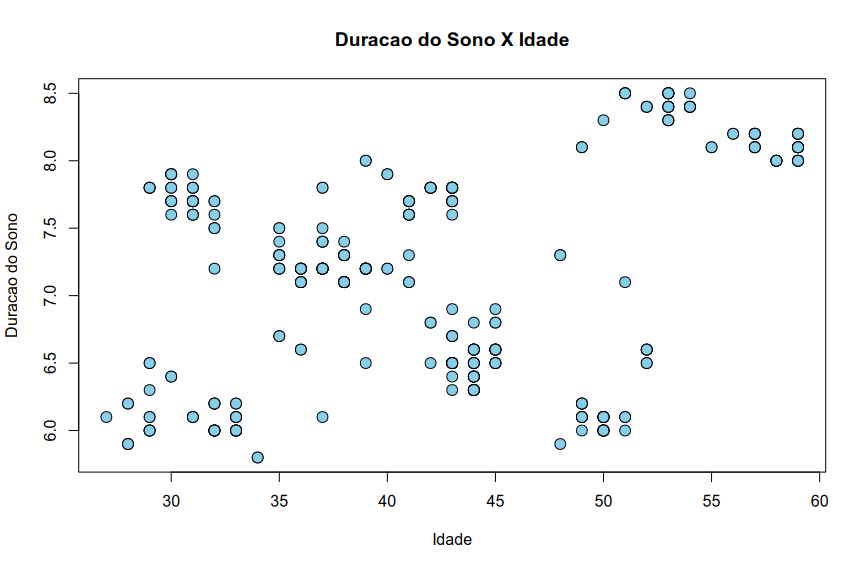
\includegraphics[width=0.8\linewidth]{figures/grafico_dispersao.png}
%     \end{figure}
% \end{frame}

% \begin{frame}{Interpretação - Gráfico de dispersão}
%     Em geral, a interpretação de um gráfico de dispersão se concentra em avaliar o comportamento de uma variável em relação à outra. 

%     Na Figura do slide anterior, podemos observar que \textbf{parece} que ao aumentar a idade, também há o aumento da duração do sono. 
% \end{frame}

% \begin{frame}[fragile]
%     \frametitle{Gráficos - Gráfico de dispersão - Exemplo no R }
    
% \begin{block}{Gráfico de dispersão no R}
% \begin{minted}[linenos=false,breaklines]{R}
% require("readxl")
% dados = read_excel(file.choose(), sheet=1) 
% duracao_sono = dados$`Duracao do Sono`
% idade = dados$Idade
% plot(x=idade, y=duracao_sono,
%      main="Duracao do Sono X Idade",
%      xlab ="Idade", ylab = "Duracao do Sono",
%      bg = "#87ceeb", # Cor dos pontos
%      cex = 1.5, # Tamanho dos pontos
%      pch=21) # Tipo do ponto      
% \end{minted}
%     \end{block}
%     \end{frame}

% \begin{frame}{Gráficos - Gráfico de setores (pizza)}
%     Consiste em dividir um círculo (pizza) em diferentes setores (fatias),
%      cada um representando a proporção do elemento analisado em relação ao conjunto de estudo. 
%     \begin{figure}
%         \centering
%         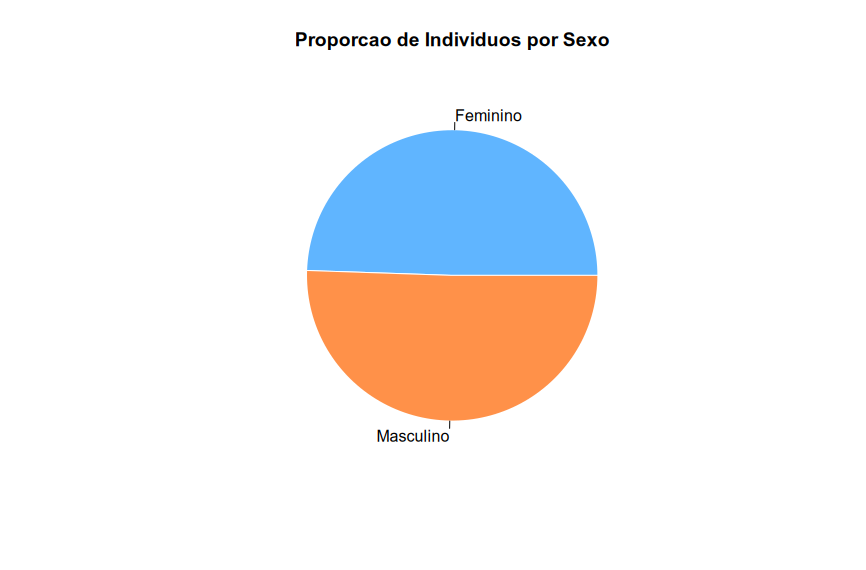
\includegraphics[width=0.8\linewidth]{figures/grafico_pizza.png}
%     \end{figure}
% \end{frame}

% \begin{frame}
%     \begin{atencao}
%         Olhando para o gráfico do slide anterior, qual sexo parece ter maior proporção?
%     \end{atencao}
    

%     \pause

%     Devido a esse problema, recomenda-se evitar o uso de gráficos de pizza. Sendo recomendado:

%     \begin{itemize}
%         \item Colocar as porcentagens por extenso caso existam poucas categorias.
%         \item Usar outro gráfico, como por exempo o gráfico de barras. 
%     \end{itemize}
% \end{frame}

% \begin{frame}[fragile]
%     \frametitle{Gráficos - Gráfico de setores (pizza) - Exemplo no R}
    
%     \begin{block}{Gráfico de pizza no R}
%     \begin{minted}[linenos=false,breaklines]{R}
% require("readxl")
% dados = read_excel(file.choose(), sheet=1) 
% sexo = dados$Sexo
% freq_sexo = table(sexo)
% pie(freq_sexo,
%     border="white", # Coloca bordas brancas
%     col=c("#60B5FF", "#FF9149"), # Cor de cada fatia
%     main = "Proporcao de Individuos por Sexo")
% \end{minted}
% \end{block}
% \end{frame}

% \begin{frame}{Gráficos - Gráfico de barras}
% \begin{itemize}
%     \item Utiliza o plano cartesiano com os valores da variável no eixo das abcissas e as frequências ou porcentagens no eixo das ordenadas. 
%     \pause
%     \item Utilizado, geralmente, para representar visualmente uma tabela de frequência.
% \end{itemize}

% \pause
% \begin{figure}
%     \centering
%     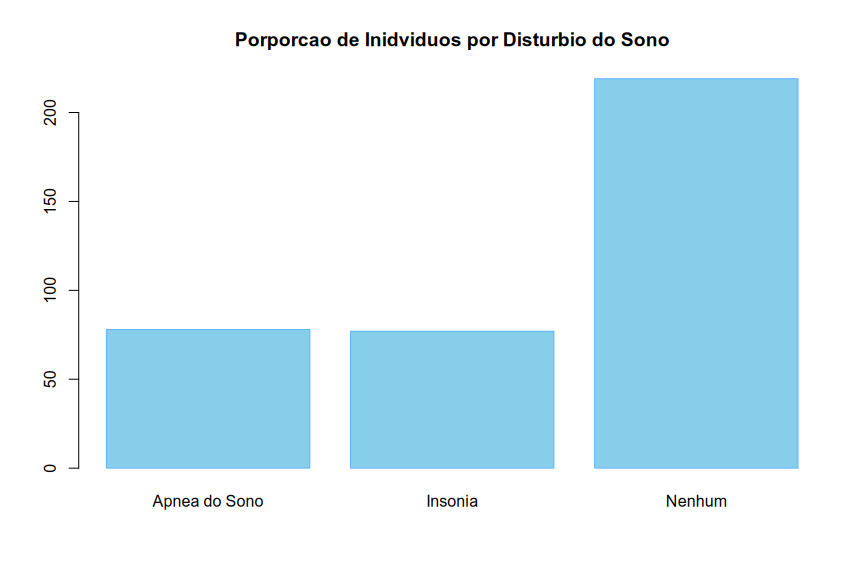
\includegraphics[width=0.8\linewidth]{figures/grafico_barras.png}
%     \caption{Gráfico de barras para a variável cidade}
% \end{figure}
% \end{frame}

% \begin{frame}{Interpretação - Gráfico de barras}

%     \begin{itemize}
%         \item No gráfico de barras, estamos interessados em entender a altura da barra referente a cada categoria analisada. 
%         \pause
%         \item Na Figura do slide anterior, podemos perceber que \textbf{parece} que temos a mesma proporção de indivíduos com apnea do sono e insonia, sendo 
%         o fato de não ter nenhum disturbio a Característica maoritariamente presente no conjunto de dados. 
%     \end{itemize}
% \end{frame}


% \begin{frame}[fragile]
% \frametitle{Gráficos - Gráfico de barras - Exemplo no R}
% \begin{block}{Gráfico de barras no R}
% \begin{minted}[linenos=false,breaklines]{R}
% require("readxl")
% dados = read_excel(file.choose(), sheet=1) 
% disturbio_sono = dados$`Disturbio do Sono`
% freq_disturbio = table(disturbio_sono)
% barplot(freq_disturbio, 
%         main="Porporcao de Inidviduos por Disturbio do Sono",
%         border="#60B5FF",# Cor do contorno das barras
%         col="#87ceeb") # Cor das barras
% \end{minted}
% \end{block}
% \end{frame}

% \begin{frame}{Gráficos - Histograma}
%     \begin{itemize}
%         \item  O histograma é bastante semelhante ao gráfico de barras.
%         \pause
%         \item  Utilizado, em geral, como uma uma representação visual da uma tabela agrupada em classes. 
%         \pause
%         \item Evidencia a distribuição de uma variável quantitativa. 
%     \end{itemize}
% \pause

% \begin{figure}
%     \centering
%     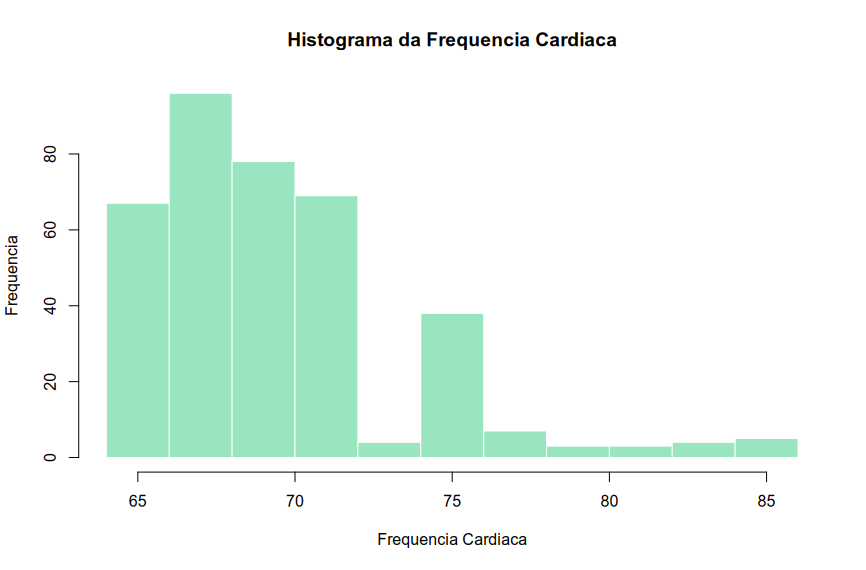
\includegraphics[width=0.8\linewidth]{figures/grafico_histograma.png}
% \end{figure}
% \end{frame}

% \begin{frame}{Interpretação - Histograma}
%     \begin{itemize}
%         \item  Ao olhar para um histograma estamos interessados em analisar a distribuição dos valores, tentando
%         perceber a concentração dos valores para a variável analisada.
%         \pause
%         \item Uma outra possibilidade é tentar identificar algum padrão, podendo relacionar com distribuições estatísticas conhecidas. 
%         \item Na Figura do slide anterior, poodemos perceber que há uma maior concentração de frequências cardiacas antes do valor 72 batimentos por minuto.  
%     \end{itemize}

% \end{frame}

% \begin{frame}[fragile]
% \frametitle{Gráficos - Histograma - Exemplo no R}
% \begin{block}{Histograma no R}
% \begin{minted}[linenos=false,breaklines]{R}
% require("readxl")
% dados = read_excel(file.choose(), sheet=1) 
% freq_cardiaca = dados$`Frequencia Cardiaca`
% hist(freq_cardiaca, 
%      main="Histograma da Frequencia Cardiaca",
%      xlab = "Frequencia Cardiaca",
%      ylab = "Frequencia",
%      breaks=8, # Numero de barras (Nem sempre)
%      col="#33CC8080", # Cor das barras
%      border=FALSE) # Elimina as bordas
% \end{minted}
% \end{block}
% \end{frame}

% \begin{frame}{Gráficos - Histograma}
%     \begin{itemize}
%         \item O argumento breaks define o número de barras, entretanto, para esse gráfico, todas as barras devem ter o mesmo tamanho. 
%         \pause
%         \item Também é possível passar uma tabela de frequencia em classes dentro da função. 
%     \end{itemize}
% \end{frame}

% \begin{frame}{Gráficos - Boxplot}
%     De forma inicial, o gráfico Boxplot apresenta a distribuição dos dados, mas, diferentemente do histograma, apresenta alguns elementos específicos, os quais
%     serão vistos posteriormente. 

%     \pause

%     \begin{figure}
%         \centering
%         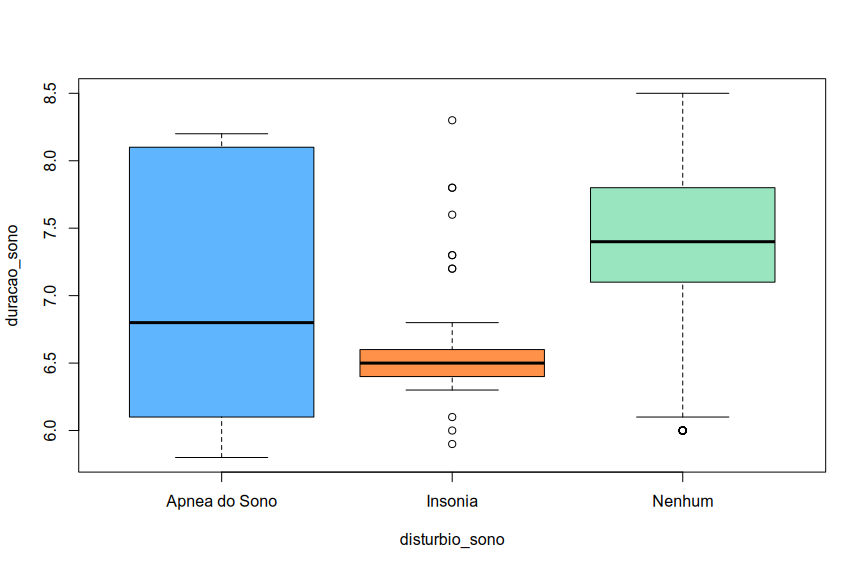
\includegraphics[width=0.8\linewidth]{figures/grafico_boxplot.png}
%     \end{figure}
% \end{frame}

% \begin{frame}[fragile]
% \frametitle{Gráficos - Extras}
% \begin{block}{Gráfico de uma função matemática}
% \begin{minted}[linenos=false,breaklines]{R}
% modulo = function(x){
%     return(abs(x))
% }
% curve(modulo,
%     -2, 2, # Intervalo do eixo x
%     ylim=c(0, 3), # Intervalo do eixo y
%     col="#60B5FF", # Cor do grafico
%     ann=FALSE) # Remove nomes nos eixos
% \end{minted}
% \end{block}
% \end{frame}

% \begin{frame}[fragile]
% \frametitle{Gráficos - Extras}
% \begin{block}{Adicionar linhas verticais e horizontais}
% \begin{minted}[linenos=false,breaklines]{R}
% modulo = function(x){
%     return(abs(x))
% }
% curve(modulo, -2, 2, ylim=c(0, 3),
%       col="#60B5FF",
%       ann=FALSE) 
% abline(h=0) # Adiciona uma linha horizontal y=0
% abline(v=0) # Adiciona uma linha vertical x=0
% \end{minted}
% \end{block}
% \end{frame}


% \begin{frame}[fragile]
%     \frametitle{Gráficos - Extras}
%     \begin{block}{Vários Gráficos em uma mesma Imagem}
%     \begin{minted}[linenos=false,breaklines]{R}
% modulo = function(x){
%     return(abs(x))
% }
% quadratica = function(x){
%     return(x^2)
% }
% curve(modulo, -2, 2, col="#60B5FF",
%       ann=FALSE, ylim=c(0, 3))
% par(new=TRUE)
% curve(quadratica, -2, 2, col="#FF9149",
%       axes=FALSE, ann=FALSE, ylim=c(0, 3))
% \end{minted}
% \end{block}
% \end{frame}

% \begin{frame}[fragile]
% \frametitle{Gráficos - Extras}
% \begin{block}{Adicionando pontos no plano cartesiano}
% \begin{minted}[linenos=false,breaklines]{R}
% modulo = function(x){
%     return(abs(x))
% }
% quadratica = function(x){
%     return(x^2)
% }
% curve(modulo, -2, 2, col="#60B5FF",
%       ann=FALSE, ylim=c(0, 3))
% par(new=TRUE)
% curve(quadratica, -2, 2, col="#FF9149",
%       axes=FALSE, ann=FALSE, ylim=c(0, 3))
% points(-1, 1, col='red', pch=19) # Adiciona um ponto vermelho no ponto (-1,1)
% points(1, 1, col='red', pch=19)  # Adiciona um ponto vermelho no ponto (1,1)      
% \end{minted}
% \end{block}
% \end{frame}

% \begin{frame}{Gráficos - Exemplos a não serem seguidos}
%     \begin{figure}
%         \centering
%         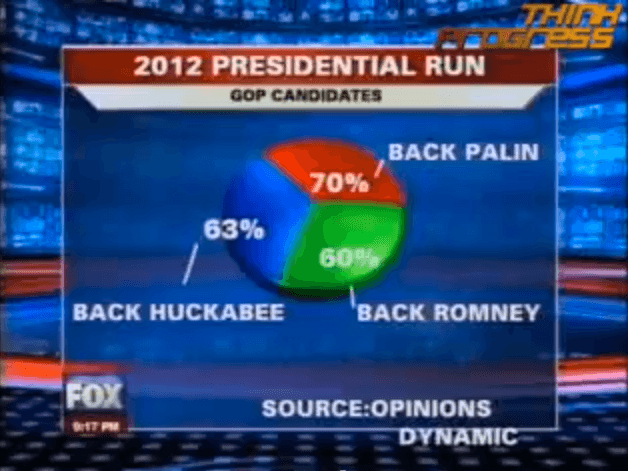
\includegraphics[width=0.8\linewidth]{figures/lie_1.png}
%     \end{figure}
% \end{frame}

% \begin{frame}{Gráficos - Exemplos a não serem seguidos}
%     \begin{figure}
%         \centering
%         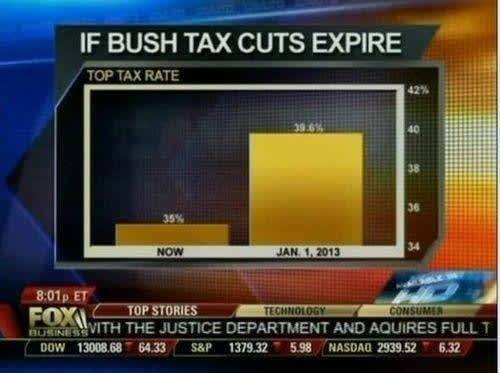
\includegraphics[width=0.8\linewidth]{figures/lie_2.jpeg}
%     \end{figure}
% \end{frame}


% \begin{frame}{Gráficos - Exemplos a não serem seguidos}
%     \begin{figure}
%         \centering
%         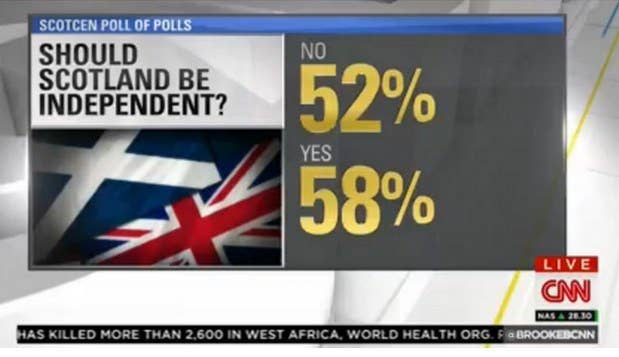
\includegraphics[width=0.8\linewidth]{figures/lie_4.jpg}
%     \end{figure}
% \end{frame}

% \begin{frame}{Gráficos - Exemplos a não serem seguidos}
%     \begin{figure}
%         \centering
%         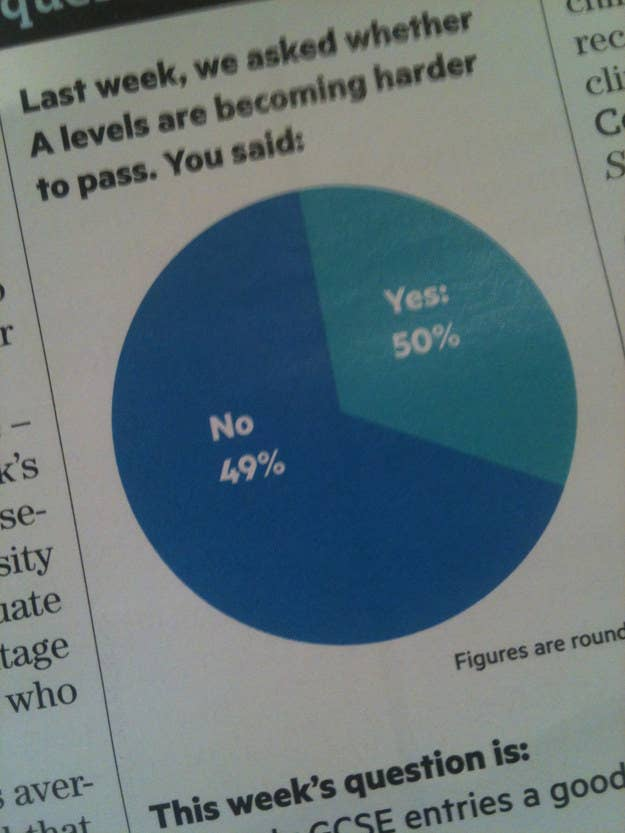
\includegraphics[width=0.5\linewidth]{figures/lie_5.jpg}
%     \end{figure}
% \end{frame}

% \begin{frame}{Gráficos - Exemplos a não serem seguidos}
%     \begin{figure}
%         \centering
%         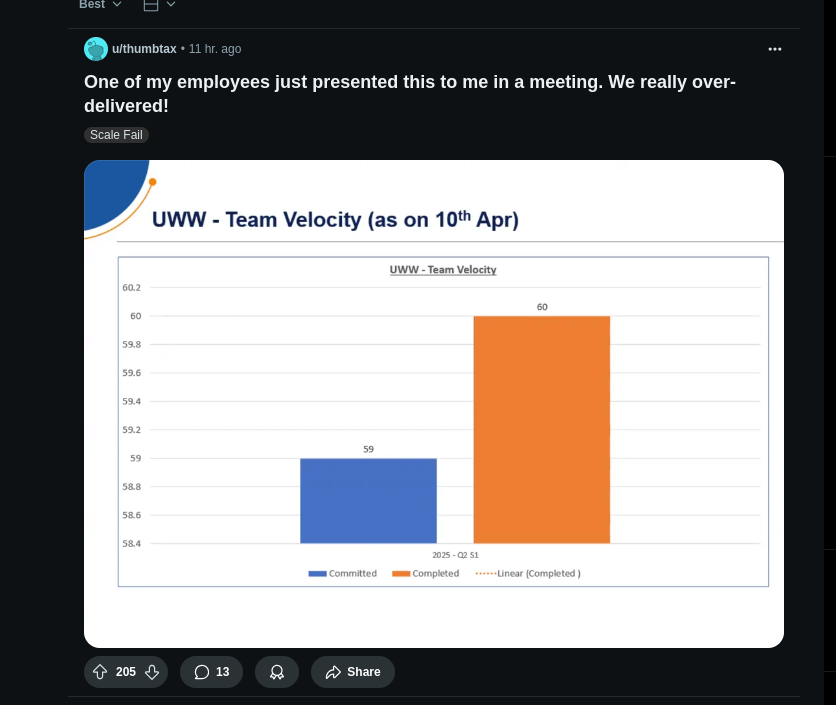
\includegraphics[width=0.8\linewidth]{figures/lie_6.png}
%     \end{figure}
% \end{frame}


% \begin{frame}{Gráficos - Exemplos a não serem seguidos}
%     \begin{figure}
%         \centering
%         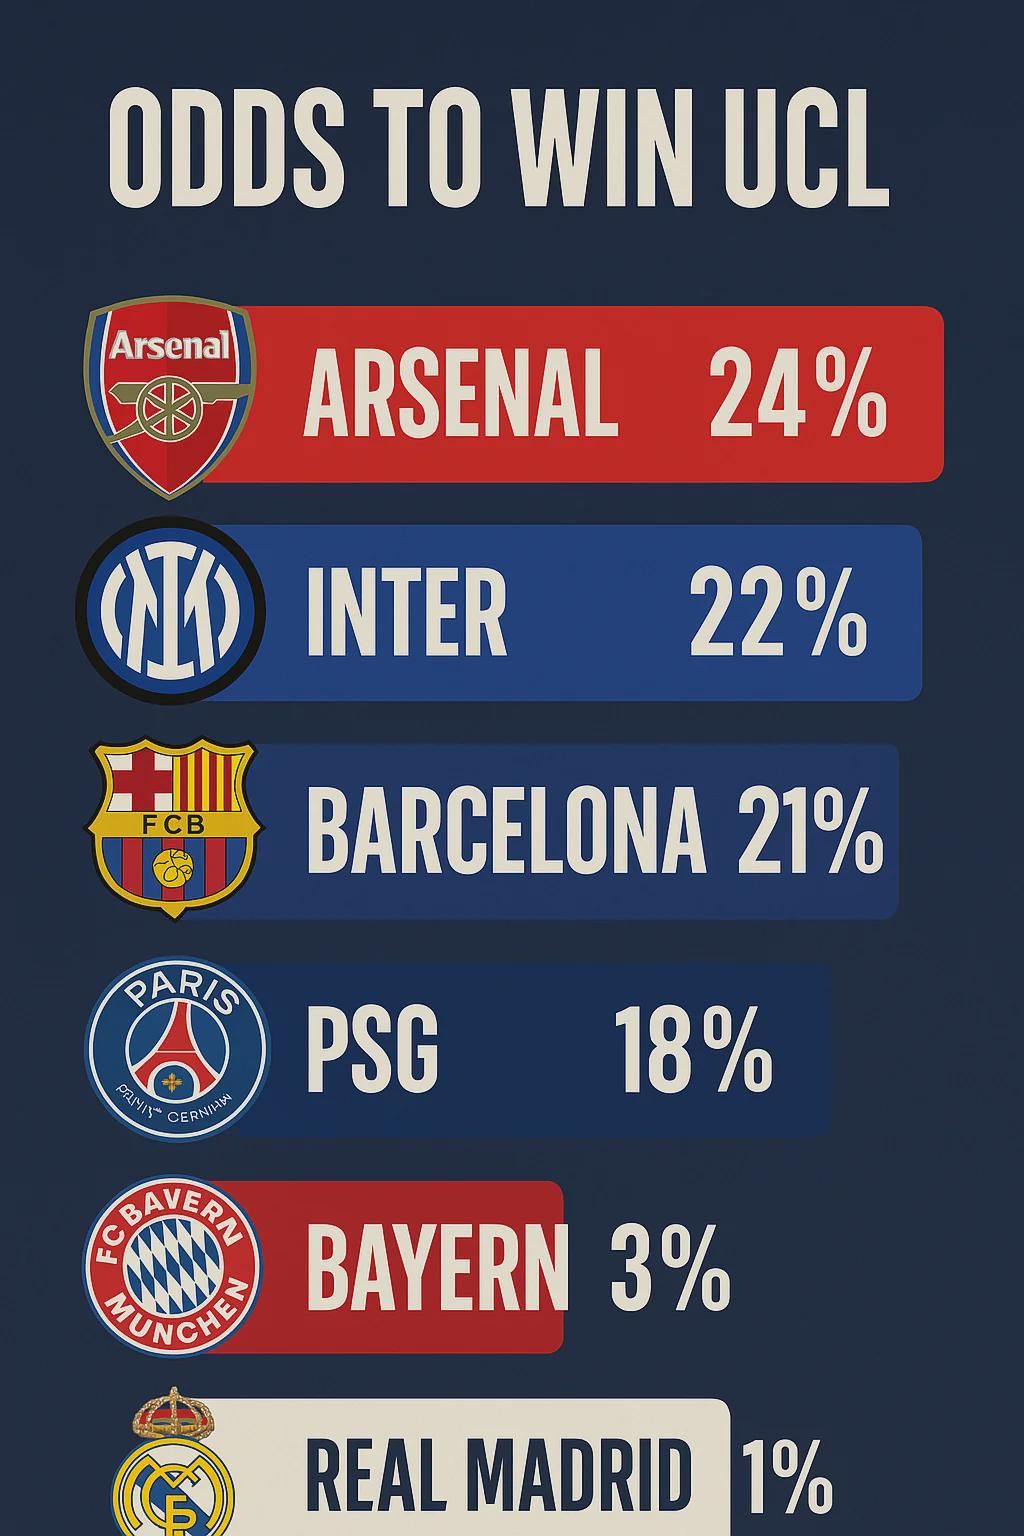
\includegraphics[width=0.4\linewidth]{figures/lie_7.jpeg}
%     \end{figure}
% \end{frame}

% \begin{frame}{Medidas de Posição}

% Podemos ter o interesse em resumir nosso conjunto de dados, apresentando um ou mais valores que de certa forma representem todo o conjunto de dados.

% Para determinar esses valores, utiliza-se as \textbf{medidas de posição central}: Média, Mediana e Moda. 

% \end{frame}

% \begin{frame}{Média Aritmética}

% Dado um conjunto de $n$ observações $x_1, x_2, \dots, x_n$ a média aritmética é definida como:

% $$\Bar{x} = \dfrac{\sum\limits_{i=1}^n x_i}{n} = \dfrac{x_1 + \dots + x_n}{n}$$

% \end{frame}

% \begin{frame}{Média Aritmética}
% \begin{exemplo}
%     Suponha que tenhamos coletado a altura de $10$ alunos de uma turma, as alturas obtidas foram as seguintes:
%     $$1,90; 1,67; 1,87; 1,55; 1,76; 1,87; 1,95; 1,66; 1,75; 1,60$$
% \end{exemplo}

% Logo, 

% {\footnotesize $$\Bar{x} = \dfrac{1,90 + 1,67 + 1,87 + 1,55 + 1,76 + 1,87 + 1,95 + 1,66 + 1,75 + 1,60}{10} = 1,76$$}
% \end{frame}

% \begin{frame}[fragile]
% \frametitle{Média Aritmética - Exemplo no R}    
% Para calcular a média de um conjunto de dados no R, utilizamos a função \textit{mean}.
% \begin{block}{Calculando a Média Aritmética no R}
% \begin{minted}[linenos=false,breaklines]{R}
% altura =  c(1.90, 1.67, 1.87, 1.55, 1.76, 1.87, 1.95, 1.66, 1.75, 1.60)
% media_altura = mean(altura)
% \end{minted}
% \end{block}
% \end{frame}

% \begin{frame}{Média Aritmética}
% \begin{exemplo}
%     Obtenha a média da Idade dos indivíduos do conjunto de dados adotado na disciplina.
% \end{exemplo}    
% \end{frame}

% \begin{frame}{Moda}
%     A moda de um conjunto de dados, representada por $x^*$, é o valor que mais se repete, 
%     ou seja, o valor mais frequente. 
%     \pause

%     \begin{atencao}
%         Um conjunto de dados pode ter mais de uma moda.
%     \end{atencao}
% \end{frame}

% \begin{frame}{Mediana}

% Seja $x_1, x_2, \dots, x_n$ um conjunto de $n$ observações, e seja $x_{(i)}, i=1, \dots, n$
% o conjunto das observações ordenadas, de modo que $x_{(1)} \leq x_{(2)} \leq \dots \leq x_{(n)}$.
% Então, a mediana $Q_2$ é definida como o valor tal que 50\% das observações são menores
% e 50\% são maiores que ela. 
% \pause
% \begin{exemplo}   

% Suponhamos que o peso de 7 crianças de uma determinada turma escolar tenha sido coletada, os pesos coletados são exibidos a seguir:

% $$28, 34, 45, 39, 42, 33, 50$$

% Obtenha a mediana desse conjunto de dados
% \end{exemplo}
% \end{frame}

% \begin{frame}{Mediana}
% Primeiramente vamos ordenar os dados:

% $$28, 33, 34, 39, 42, 45,  50$$

% \pause 
% Logo, a mediana será o valor $39$

% \end{frame}

% \begin{frame}{Mediana}
% \begin{exemplo}
% Retomemos o exemplo das alturas dos alunos, temos os seguintes dados:

% $$1,90; 1,67; 1,87; 1,55; 1,76; 1,87; 1,95; 1,66; 1,75; 1,60$$

% \end{exemplo}

% Para calcular a mediana, primeiramente vamos ordenar os dados:

% $$ 1,55; 1,60; 1,66; 1,67; 1,75; 1,76;  1,87;  1,87; 1,90; 1,95$$

% \pause

% Temos 10 elementos, logo, não conseguimos encontrar o valor que divide exatamente ao meio o conjunto de dados, nesse caso, a mediana é dada pela média dos elementos que ocupam a posição $\frac{n}{2}$ e $\frac{n}{2} +1 $.

% $$Q_2 = \dfrac{1,75 + 1,76}{2} = 1,755$$
% \end{frame}

% \begin{frame}{Mediana}
% Portanto, 
% $$Q_2 = \begin{cases}
%     x_{\left(\frac{n+1}{2} \right)} & \text{se n é impar}\\
%     \dfrac{x_{\left(\frac{n}{2}\right)} + x_{\left(\frac{n}{2} + 1 \right)} }{2} & \text{se n é par}\\
% \end{cases}$$
% \end{frame}

% \begin{frame}[fragile]
% \frametitle{Médiana - Exemplo no R}   
% Para obter a mediana de um conjunto de dados no R, basta usar a função \textit{median}
% \begin{block}{Calculando a Mediana no R}
% \begin{minted}[linenos=false,breaklines]{R}
% require("readxl")
% dados = read_excel(file.choose(), sheet=1) 
% idades = dados$Idade
% mediana_idade = median(idades)
% \end{minted}
% \end{block}
% \end{frame}

% \begin{frame}{Média X Mediana}

% \begin{itemize}
%     \item Imagine que você precisa atravessar um lago e existe uma placa que diz: Altura média do lago: $1,5$ metros. Você o atravessaria?
%     \pause
%     \item Dependendo do conjunto de dados, nem sempre a média é uma boa medido da resumo. A média é fortemente influenciada por valores aberrantes (outliers). 
% \end{itemize}

% \pause

% \begin{exemplo}
%     Os seguintes dados referentes aos salários (em R\$) de cinco funcionários de uma firma: $$136; 210; 350; 360; 2500$$ Calcule o salario médio. 
% \end{exemplo}

% \end{frame}

% \begin{frame}{Média X Mediana}
%     No caso do slide anterior, o salário médio é igual a $R\$ 647,20$. No entanto, esse valor não representa, de forma adequada, os salários mais
%     baixos e os salários mais altos, isso porque o mais alto é muito diferente dos demais.
     
% \end{frame}

% \begin{frame}{Média X Mediana}
%     \begin{itemize}
%         \item Por outro lado, a mediana desse conjunto de dados é o valor $350$, que indica que metade dos valores é menor que $350$ e a outra metade maior. 
%         \item Ainda assim, não conseguimos capturar o quanto menor ou maior são. 
%     \end{itemize}
% \end{frame}

% \begin{frame}{Observações}
% \begin{itemize}
%     \item Quando a média é próxima a mediana dizemos que isso é um indicativo de que a amostra não apresenta pontos aberrantes (possíveis outliers).
%     \item A média é fortemente influenciada pela presença de pontos aberrantes, enquanto a mediana não é.
% \end{itemize}
    
% \end{frame}

% \begin{frame}{Média Ponderada}
%     A média aritmética ponderada de números $x_1, x_2, \dots, x_n$ com pesos
%     $w_1, w_2, \dots, w_n$ é definida como:

%     $$\bar{x}_w = \dfrac{w_1x_1 + w_2x_2 + \dots + w_nx_n }{w_1 +w_2 + \dots + w_n} = \dfrac{\sum_{i=1}^n w_i x_i}{\sum_{i=1}^n w_i}$$
% \end{frame}

% \begin{frame}{Quartis - Elementos fundamentais}
%     \begin{itemize}
%         \item O primeiro quartil, que indicaremos por $Q_1$, deixa 25\% das observações abaixo e 75\% acima dele. 
%         \pause
%         \item A mediana é o segundo quartil
%         \pause
%         \item O terceiro quartil, $Q_3$, deixa 75\% das observações abaixo e 25\% acima dele. 
%     \end{itemize}
    
% \end{frame}

% \begin{frame}{Quartis - Elementos adicionais}
%     \begin{itemize}
%         \item Amplitude Interquartil (AIQ) = $Q_3 - Q_1$
%         \pause
%         \item Limite Superior = $Q_3 + 1,5 \cdot AI$
%         \pause
%         \item Limite Inferior = $Q_1 - 1,5 \cdot AI$
%     \end{itemize}
   
% \end{frame}

% \begin{frame}{Quartis - Cálculo dos quartis}
%     $$Q_1 = x_{\left(\frac{1}{4}(n+1) \right)}$$
%     \pause
%     $$Q_3 =  x_{\left(\frac{3}{4}(n+1)\right)} $$
%     \textcolor{red}{Importante:} Se o valor obtido não for um inteiro, fazer uma média do elemento que ocupa a parte inteira e seu sucessor.
% \end{frame}

% \begin{frame}[fragile]
% \frametitle{Quartis - Exemplo no R}   
% Para obter os quartis de um conjunto de dados no R, utilizamos a função \textit{quantile}.
% \begin{block}{Variância no R}
% \begin{minted}[linenos=false,breaklines]{R}
% require("readxl")
% dados = read_excel(file.choose(), sheet=1) 
% duracao_sono = dados$`Duracao do Sono`
% q1 = quantile(duracao_sono, 0.25) # Primeiro quartil
% q3 = quantile(duracao_sono, 0.75) # Terceiro quartil
% \end{minted}
% \end{block}
% \end{frame}

% \begin{frame}{Revisitando o Boxplot}
%     \begin{figure}
%     \centering
%     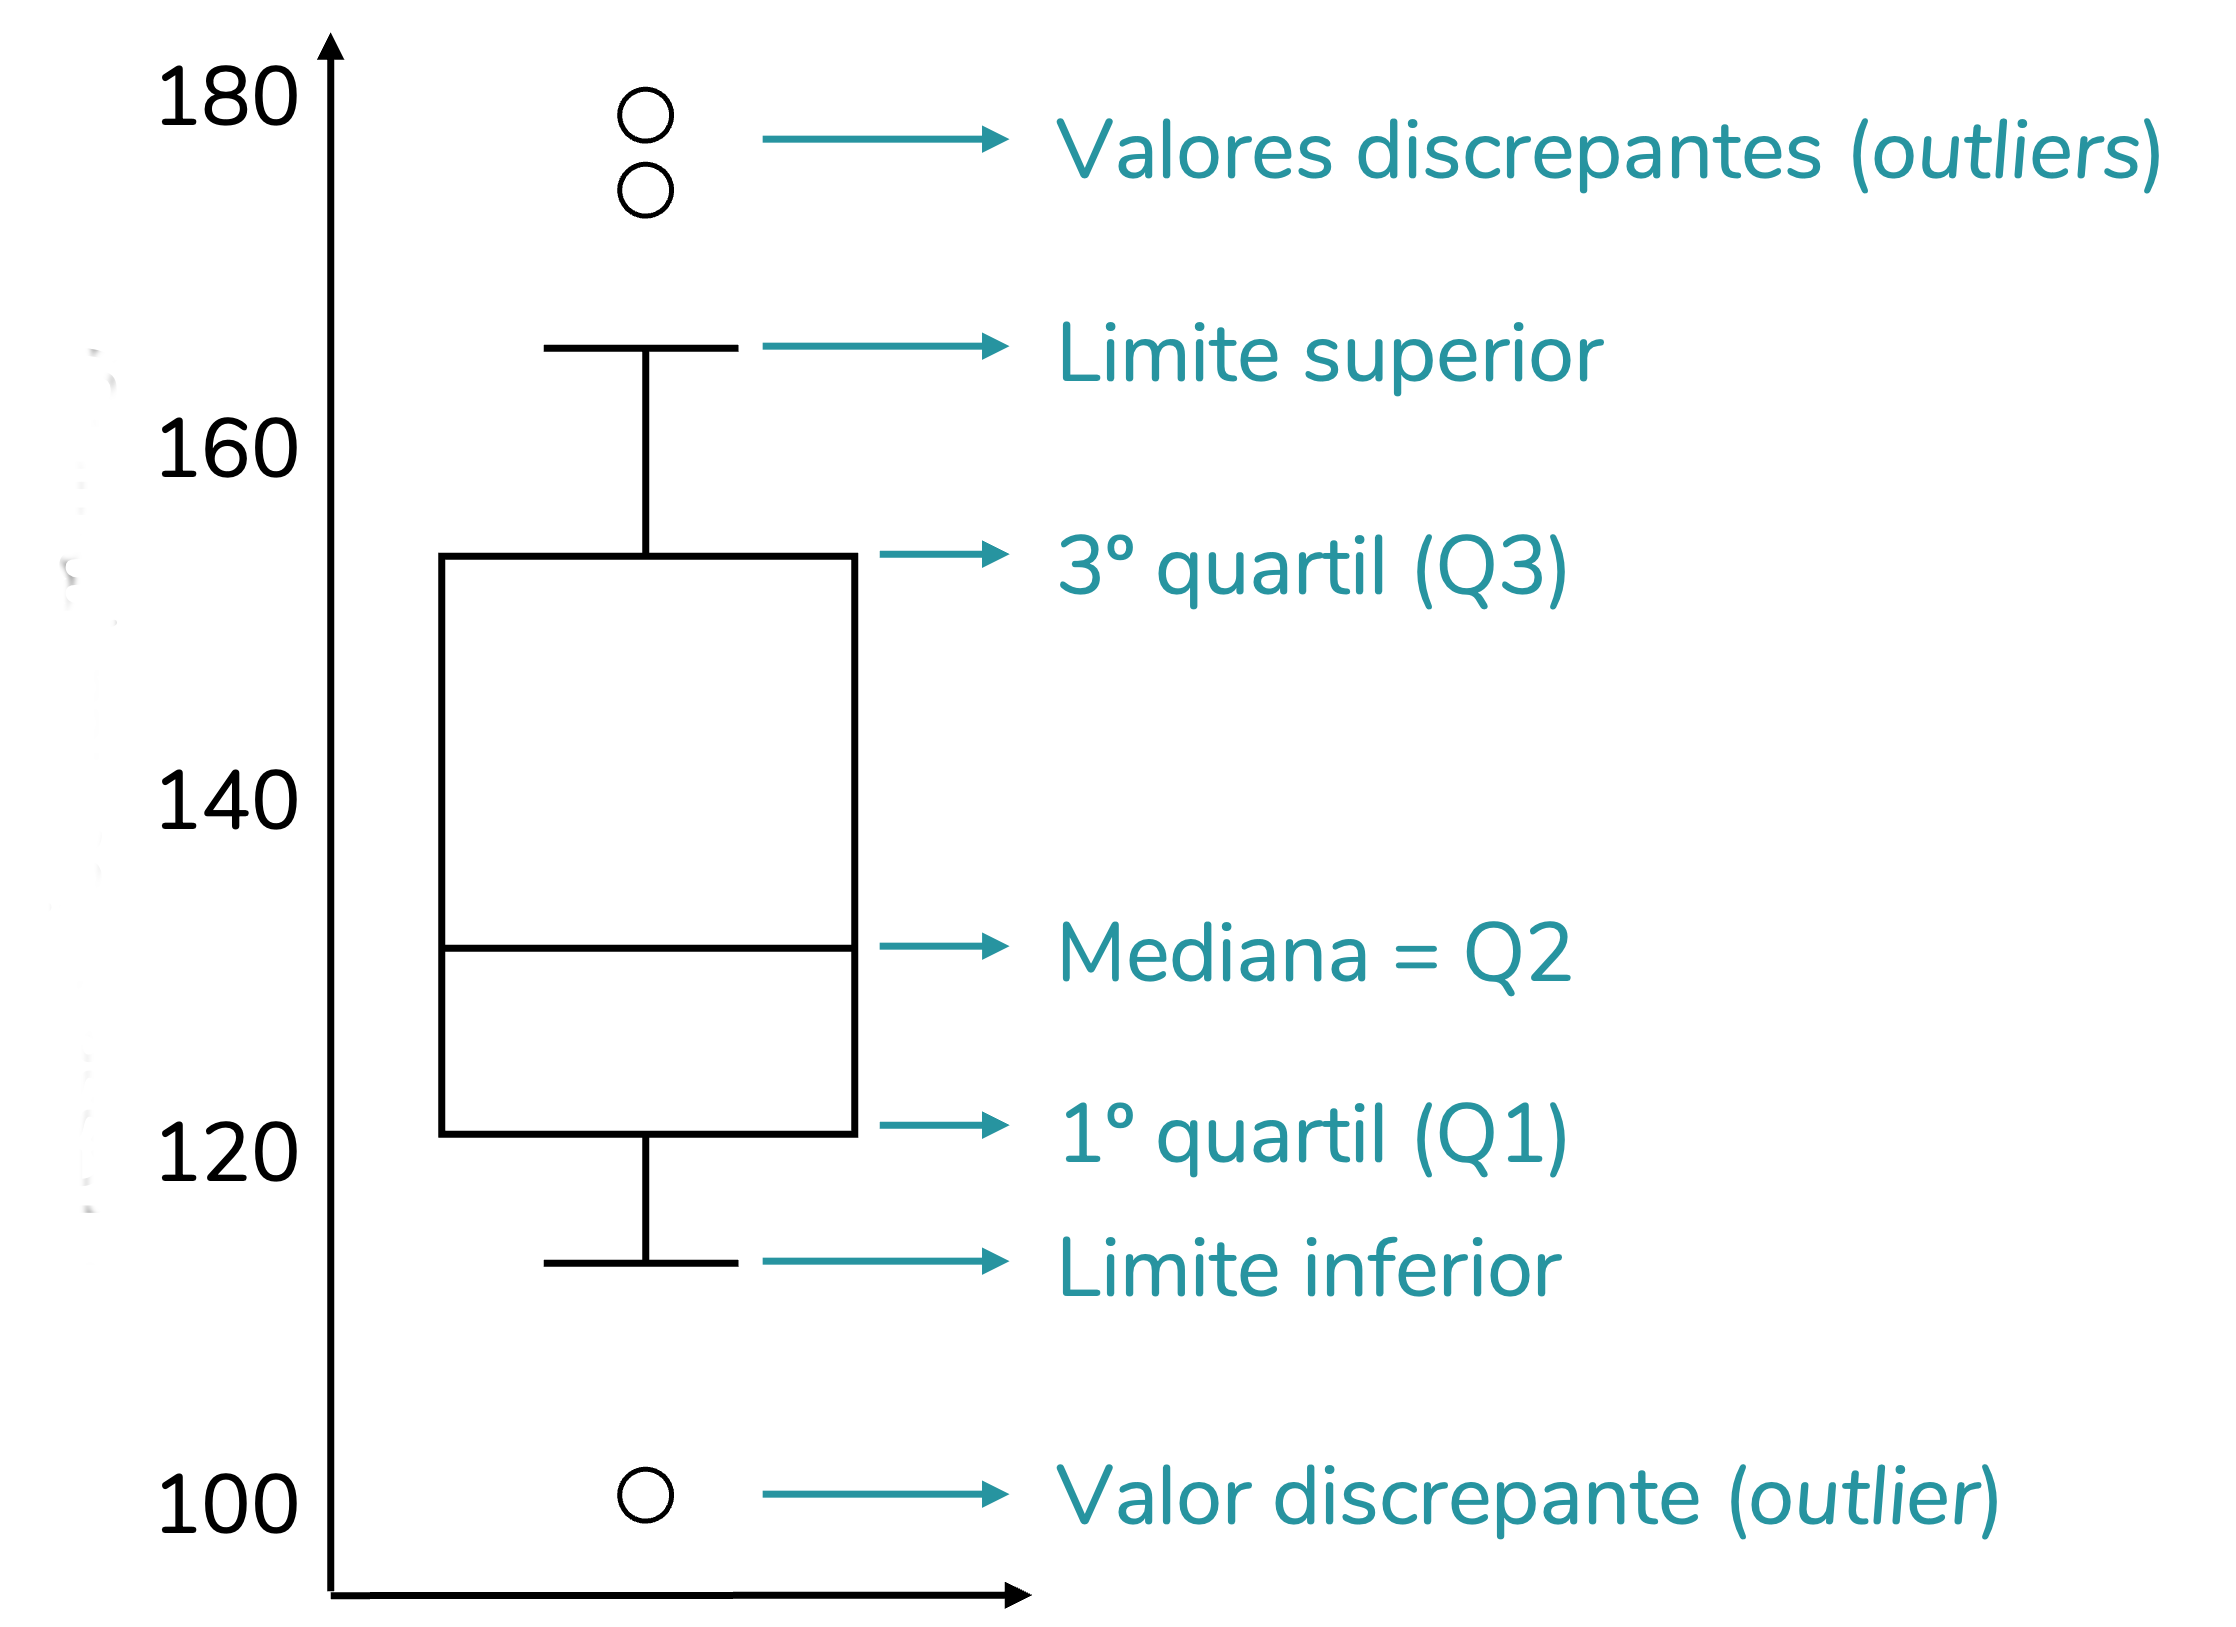
\includegraphics[width=0.6\linewidth]{figures/boxplot.png}    
%     \end{figure}
% \end{frame}

% \begin{frame}[fragile]
% \frametitle{Boxplot - Exemplo no R}   
% \begin{block}{Gráfico Boxplot no R}
% \begin{minted}[linenos=false,breaklines]{R}
% require("readxl")
% dados = read_excel(file.choose(), sheet=1) 
% disturbio_sono = dados$`Disturbio do Sono`
% duracao_sono = dados$`Duracao do Sono`
% boxplot(duracao_sono ~ disturbio_sono,
%         col=c("#60B5FF", "#FF9149", "#33CC8080"))
% \end{minted}
% \end{block}
% \end{frame}
% \begin{frame}{Medidas de dispersão}

% Muitas vezes estamos interessados em entender o comportamento dos dados e as medidas de posição não são suficientes:

% \begin{exemplo}
%     Calcule a média dos seguintes conjuntos de dados:
%     $$salarios_1 = 2.000,00 ; 3.500,00 ; 4.900,00 ; 3.100,00 $$
%     $$salarios_2 = 3.375,00 ; .3375,00; 3.375,00; 3.375,00$$
% \end{exemplo}
% \end{frame}

% \begin{frame}{Medidas de dispersão}
%     \begin{exemplo}
%         Calcule a mediana dos seguintes conjuntos de dados:
%         $$salarios_1 = 2.000,00 ; 3.500,00 ; 4.900,00 ; 3.100,00; 4.100,00 $$
%         $$salarios_2 = 2.000,00 ; 3.500,00 ; 70.900,00 ; 3.100,00; 32.000,00 $$
%     \end{exemplo}
% \end{frame}

% \begin{frame}
% Em ambos os casos anteriores, percebemos que a Média e Mediana não são suficientes para descrever o comportamento dos dados. Devido a isso, 
% trabalharemos agora com medidas de dispersão, sendo elas: Amplitude, Devio médio absoluto, Variância, Desvio Padrão e Coeficiente de Variação.
% \end{frame}


% \begin{frame}{Amplitude}
%     A amplitude de um conjunto de dados é a distância entre o maior valor e o menor valor.
%     \pause
%     $$\Delta_{total} = V_{max} - V_{min}$$
%     \pause
%     A amplitude nos dá uma ideia do intervalo de possíveis valores que a variável analisada pode assumir. 
% \end{frame}

% \begin{frame}[fragile]
% \frametitle{Amplitude - Exemplo no R}   
% Para calcular a amplitude de um conjunto de dados no R, utilizamos a função \textit{var}.
% \begin{block}{Amplitude no R}
% \begin{minted}[linenos=false,breaklines]{R}
% require("readxl")
% dados = read_excel(file.choose(), sheet=1) 
% duracao_sono = dados$`Duracao do Sono`
% amplitude_duracao_sono = max(duracao_sono) - min(duracao_sono)
% \end{minted}
% \end{block}
% \end{frame}

% \begin{frame}{Desvio médio absoluto}

%  O desvio médio absoluto de um conjunto de dados $x_1, x_2, \dots, x_n$ é definido por:
% $$DMA(X) = \dfrac{\sum\limits_{i=1}^n |x_i - \Bar{x}|}{n}$$

% \pause 
% \begin{itemize}
%     \item O desvio médio tem como objetivo verificar quanto os valores, em média, estão se distanciando da média.
%     \pause
%     \item Note que o desvio médio absoluto é sempre um valor positivo. 
% \end{itemize}
% \pause
% \begin{exemplo}
%     Calcule o desvio médio para os salários dos exemplos anteriores. 
% \end{exemplo}    

% \end{frame}

% \begin{frame}{Variância}
%     A variância $\sigma^2$ de um conjunto de dados $x_1, x_2, \dots, x_n$ é definida por 
%     $$\sigma^2 = \dfrac{\sum\limits_{i=1}^n (x_i - \Bar{x})^2}{n}$$
% \pause
% \begin{itemize}
%     \item Perceba que a variância é bastante semelhante ao desvio médio absoluto, no entanto, penaliza grandes desvios. 
%     \pause
%     \item Observe que a variância é sempre um número \textbf{positivo}.
%     \pause
%     \item Note que a variância \textbf{não} fornece um valor na mesma unidade de medida dos dados. 
%     \pause
%     \item A variância não tem interpretação prática direta, podendo ser utilizada como comparação. 
% \end{itemize}
% \end{frame}

% \begin{frame}{Variância}
% \begin{exemplo}
%     Calcule a variância para os salários dos exemplos anteriores. 
% \end{exemplo}    
% \end{frame}

% \begin{frame}[fragile]
%     \frametitle{Variância - Exemplo no R}   
%     Para calcular a variância de um conjunto de dados no R, utilizamos a função \textit{var}.
%     \begin{block}{Variância no R}
%     \begin{minted}[linenos=false,breaklines]{R}
%     require("readxl")
%     dados = read_excel(file.choose(), sheet=1) 
%     duracao_sono = dados$`Duracao do Sono`
%     var_duracao_sono = var(duracao_sono)
%     \end{minted}
%     \end{block}
% \end{frame}

% \begin{frame}{Desvio padrão}

% O desvio padrão de um conjunto de dados $x_1, x_2, \dots, x_n$ é definido como a raiz 
% quadrada da variância:
% \pause
% $$\sigma =\sqrt{\sigma^2}$$
% \pause

% \begin{itemize}
%     \item Diferentemente da variância, o desvio padrão possui interpretação prática, pois ele volta o valor para a unidade de medida dos dados.
%     \pause
%     \item Interpretamos o desvio padrão como quanto, em média, os valores do conjunto de dados estão se ditanciando da média. 
%     \pause
%     \item Note que, apesar de interpretável, é difícil dizer se temos um desvio padrão alto ou baixo, mas, com o auxilio da amplitude, podemos tirar boas conclusões. 
% \end{itemize}
% \end{frame}

% \begin{frame}{Coeficiente de variação}
% Dado um conjunto de observações $x_1, x_2, \dots, x_n$; o coeficiente de variação
% (CV) é definido como a razão entre o desvio-padrão dos dados e sua média,
% ou seja,

%  $$CV = \dfrac{\sigma}{\Bar{x}}$$

%  \begin{itemize}
%     \item Em geral, multiplica-se o valor do CV por 100 para ter um valor percentual. 
%     \pause
%     \item Quanto menor for o valor do CV, mais homogêneo é um conjunto de dados.
%  \end{itemize}
% \end{frame}

% \begin{frame}{Coeficiente de variação}
%     Podemos adotar o seguinte critério:
%     \begin{itemize}
%         \item $CV < 0,10 \implies$ variabilidade baixa 
%         \item $0,10 \leq CV < 0,20 \implies$ variabilidade intermediária
%         \item $0,20 \leq CV < 0,30 \implies$ variabilidade alta
%         \item $CV \geq 0,30 \implies$ variabilidade muito alta
%     \end{itemize}

%     \textbf{Observação: Só podemos calcular o CV quando a média amostral for diferente de zero.}
% \end{frame}

% \begin{frame}{Escores padronizados}
%     Suponhamos que tenha sido feito um estudo visando entender o desempenho dos alunos do curso de Engenharia Química no curso de Cálculo em comparação com o curso de Estatística. 
%     \pause
%     \vspace{5px}
    
%     As notas de 9 alunos da turma foram coletadas e são apresentadas abaixo:

%     \centering
%     \begin{tabular}{lccccccccc}
%     \toprule
%     Aluno & 1 & 2 & 3 & 4 & 5 & 6 & 7 & 8 & 9 \\
%     \midrule
%     Estatística & 6 & 4 & 5 & 7 & 8 & 5 & 5 & 5 & 7 \\
%     Cálculo     & 6 & 8 & 9 & 10 & 7 & 7 & 8 & 9 & 3 \\
%     \bottomrule
%     \end{tabular}

%     Olhando para as notas, será que tirar 6 em Estatística tem o mesmo "peso" que tirar 6 em Cálculo?
% \end{frame}

% \begin{frame}{Escores Padronizados}
%     \centering
%     \begin{tabular}{lccccccccc}
%     \toprule
%     Aluno & 1 & 2 & 3 & 4 & 5 & 6 & 7 & 8 & 9 \\
%     \midrule
%     Estatística & 6 & 4 & 5 & 7 & 8 & 5 & 5 & 5 & 7 \\
%     Cálculo     & 6 & 8 & 9 & 10 & 7 & 7 & 8 & 9 & 3 \\
%     \bottomrule
%     \end{tabular}

%     Vamos calcular a média das notas de cada um dos cursos:
%     $$\bar{x}_{E} = \dfrac{6 + 4 + 5 + 7 + 8 + 5 + 5 + 5 + 7}{9} = \dfrac{52}{9} = 5,78$$
%     \pause
%     $$\bar{x}_{C} = \dfrac{6 + 8 + 9 + 10 + 7 + 7 + 8 + 9 + 3}{9} = \dfrac{67}{9} = 7,44$$

%     \pause
%     \begin{itemize}
%         \item Podemos perceber que, o aluno 1, por exemplo, ficou acima da média em Estatística, mas abaixo da média em Cálculo.
%         \pause
%         \item Outra forma de verificar essa afirmação é por meio do \textbf{desvio}.
%     \end{itemize}
% \end{frame}

% \begin{frame}{Escores Padronizados - Desvio}
%     O desvio de uma observação $x_i$ em torna da média é definido como:

%     $$d_i = x_i - \bar{x}$$

%     \pause

%     Calculando os desvios da nota do primeiro aluno, temos:

%     $$d_{E_1} = 6 - 5,78 = 0,22$$
%     $$d_{C_1} = 6 - 7,44 = -1,44$$

%     \pause

%     \begin{itemize}
%         \item Dessa forma, temos que o aluno 1 ficou, aproximadamente, $0,22$ pontos acima da média em Cálculo e 1,44 abaixo da média em Estatística.  
%         \pause
%         \item Ainda asssim, não temos como comparar se o desempenho do aluno foi melhor em Estatística ou em Cálculo, pois, novamente, as médias são diferentes. 
%     \end{itemize}
% \end{frame}

% \begin{frame}{Escores Padronizados}
%     \centering
%     \begin{tabular}{lccccccccc}
%     \toprule
%     Aluno & 1 & 2 & 3 & 4 & 5 & 6 & 7 & 8 & 9 \\
%     \midrule
%     Estatística & 6 & 4 & 5 & 7 & 8 & 5 & 5 & 5 & 7 \\
%     Cálculo     & 6 & 8 & 9 & 10 & 7 & 7 & 8 & 9 & 3 \\
%     \bottomrule
%     \end{tabular}

%     Vamos calcular o desvio padrão das notas de cada um dos cursos. 

%     $$\sigma^2_{E} = 1,51 \implies \sigma_{E} = 1,23$$
%     \pause
%     $$\sigma^2_{C} = 3,80 \implies \sigma_{C} = 1,95$$

%     \pause
%     \begin{itemize}
%         \item Qual disciplina apresenta maior variabilidade das notas?
%         \pause
%         \item Faça o cálculo da variância manualmente e verifique os resultados apresentados nesse slide. 
%     \end{itemize}
% \end{frame}

% \begin{frame}{Escores Padronizados}

%     O escore padronizado de uma observação $x_i$ é definido como:

%     $$z_i = \dfrac{x_i - \bar{x}}{\sigma_x}$$

%     \pause

%     \begin{itemize}
%         \item Ao dividirmos pelo desvio padrão, a escala passa a ser definida em termos do desvio padrão e cada escore padronizado nos informa que a observação está 
%         acima ou abaixo da média por um determinado número de desvios-padrão. Dessa forma, removemos o efeito das médias e o fato das variabilidades serem diferentes. 
%         \item \textcolor{red}{Importante}: A média dos escores padronizados é, independente do conjunto de dados, sempre igual a $0$ e a variância igual a $1$.
%     \end{itemize}
% \end{frame}

%     \begin{frame}{Escores Padronizados}
%      Vamos analisar agora as notas de Estatística e Cálculo em termos dos escores padronizados:

%      \centering
%      \resizebox{\textwidth}{!}{%
%      \begin{tabular}{llccccccccc}
%      \toprule
%      \multicolumn{2}{c}{Aluno} & 1 & 2 & 3 & 4 & 5 & 6 & 7 & 8 & 9 \\
%      \midrule
%      \multirow{2}{*}{Estatística} & Nota   & 6 & 4 & 5 & 7 & 8 & 5 & 5 & 5 & 7 \\
%                                   & Escore & 0{,}18 & -1{,}45 & -0{,}63 & 1{,}00 & 1{,}81 & -0{,}63 & -0{,}63 & -0{,}63 & 1{,}00 \\
%      \midrule
%      \multirow{2}{*}{Cálculo}     & Nota   & 6 & 8 & 9 & 10 & 7 & 7 & 8 & 9 & 3 \\
%                                   & Escore & -0{,}74 & 0{,}29 & 0{,}80 & 1{,}13 & -0{,}23 & -0{,}20 & 0{,}29 & 0{,}80 & -3{,}28 \\
%      \bottomrule
%      \end{tabular}
%      }
    
%     \begin{itemize}
%         \item Podemos perceber que a nota 6 está, aproximadamente, $0,18$ desvios-padrão acima da média em Estatística
%          e aproximadamente $0,74$ desvios-padrão abaixo da média das notas de Cálculo. 
%          \item Perceba que tirar a nota 10 em Cálculo é menos "surpreendente" que tirar 8 em Estatística.  
%     \end{itemize}
% \end{frame}

% \begin{frame}{Escores Padronizados - Teorema de Chebyshev}
%     Para qualquer distribuição de dados, pelo menos $(1 - 1/z^2)$ dos dados estão dentro de $z$ desvios-padrão da média, onde $z$ é qualquer valor maior que 1. 
%     Ou seja, pelo menos (1-1/z^2) dos dados estão no intervalo $\[\bar{x} - z\sigma; \bar{x} + z\sigma\]$.

% \end{frame}

% \begin{frame}{Escores Padronizados - Teorema de Chebyshev}
%     Exemplos:
%     \begin{itemize}
%         \item Para $z=2$ temos que $1-1/z^2 = 3/4 = 75\%$ dos dados estão dentro de dois desvios-padrão da média. Ou, equivalentemente, 
%         75\% dos escores padronizados estão no intervalo $(-2,2)$. 
%         \pause
%         \item Para $z=3$  que $1-1/z^2 = 8/9 = 89\%$ dos dados estão dentro de três desvios-padrão da média. Ou, equivalentemente, 
%         89\% dos escores padronizados estão no intervalo $(-3,3)$. 
%         \pause
%         \item Para $z=4$  que $1-1/z^2 = 15/16 = 93,75\%$ dos dados estão dentro de quatro desvios-padrão da média. Ou, equivalentemente, 
%         93,75\% dos escores padronizados estão no intervalo $(-4,4)$. 
%     \end{itemize}
% \end{frame}

% \begin{frame}{Covariância e Correlação}
%     \begin{itemize}
%         \item  Até agora, vimos como analisar medidas referentes a uma única variável. Entretanto, na prática, 
%         podemos nos deparar com situaçãos nas quais se faz interessante estudar a relação entre duas ou mais
%         variáveis. 
%         \pause
%         \item    Nesse sentido, surge a Covariância e a Correlação, que são medidas usadas para analisar a relação entre duas ou mais variáveis.  
%     \end{itemize}
% \end{frame}

% \begin{frame}{Covariância}
%     A covariância entre duas variáveis $X$ e $Y$ é definida por:

%     $$Cov(X,Y) = \dfrac{\sum_{i=1}^n (x_i - \bar{x})(y_i - \bar{y}) }{n}$$

%     \pause

%     \begin{itemize}
%         \item A covariância mede o grau de associação \textbf{linear} entre as variáveis.
%         \pause
%         \item A unidade de medida é dada pelo produto das unidades de medida das variáveis X e Y.
%         \pause
%         \item  \textcolor{red}{Importante}: A covariância depende da escala dos dados, o que faz com que seja difícil estabelecer comparações. 
%         \pause
%         \item  Seus valores podem variar de $-\infty$ a $\infty$
%     \end{itemize}
% \end{frame}


% \begin{frame}[fragile]
%     \frametitle{Covariância - Exemplo no R}   
%     Para calcular a covariãncia entre duas variáveis no R, utilizamos a função \textit{cov}.
%     \begin{block}{Covariância no R}
%     \begin{minted}[linenos=false,breaklines]{R}
%     dados = read.csv(file.choose())
%     duracao_sono = dados$`Duracao do Sono`
%     idade = dados$Idade
%     cov_dsono_idade = cov(duracao_sono, idade)
%     \end{minted}
%     \end{block}
% \end{frame}

% \begin{frame}{Impacto da escala dos dados no cálculo da covariância}
%     \begin{itemize}
%         Exemplo no R, arquivo: escala\_covariancia.R 
%     \end{itemize}
% \end{frame}

% \begin{frame}{Coeficiente de correlação}
%     O coeficiente de correlação entre duas variáveis $X$ e $Y$ é definido por:

%     $$Corr(X,Y) = \rho(X,Y) = \dfrac{1}{n} \sum_{i=1}^n \left( \dfrac{x_i - \bar{x}}{\sigma_X}\right) \left( \dfrac{y_i - \bar{y}}{\sigma_Y}\right)$$

%     \pause
%     \begin{itemize}
%         \item O coeficiente de correlação também mede o grau de associação \textbf{linear} entre as variáveis.
%         \pause
%         \item  O coeficiente de correlação \textbf{não} depende da escala dos dados, permitindo comparações. 
%         \pause
%         \item Seus valores podem variar entre $-1$ e $1$.
%     \end{itemize}
% \end{frame}

% \begin{frame}{Classificação do coeficiente de correlação}
    
% \begin{table}[H]
% \centering
% \begin{tabular}{|c|l|}
% \hline
% \textbf{Valor de $\rho$ (+ ou –)} & \textbf{Interpretação} \\ \hline
% 0{,}00 a 0{,}19 &  Correlação bem fraca \\ \hline
% 0{,}20 a 0{,}39 &  Correlação fraca \\ \hline
% 0{,}40 a 0{,}69 &  Correlação moderada \\ \hline
% 0{,}70 a 0{,}89 &  Correlação forte \\ \hline
% 0{,}90 a 1{,}00 &  Correlação muito forte \\ \hline
% \end{tabular}
% \end{table}
% \end{frame}

% \begin{frame}[fragile]
% \frametitle{Correlação - Exemplo no R}   
%     Para calcular o coeficiente de correlação entre duas variáveis no R, utilizamos a função \textit{cor}.
%     \begin{block}{Correlação no R}
%     \begin{minted}[linenos=false,breaklines]{R}
%     dados = read.csv(file.choose())
%     duracao_sono = dados$`Duracao do Sono`
%     idade = dados$idade
%     cor_dsono_idade = cor(duracao_sono, idade)
%     \end{minted}
%     \end{block}
% \end{frame}

% \begin{frame}{Correlação \textbf{Linear} ( Apenas Linear)}
%     Exemplo no R, arquivo: correlacao\_linear.R
% \end{frame}

% \begin{frame}{Correlação não implica causalidade}
%     \begin{figure}
%         \centering
%         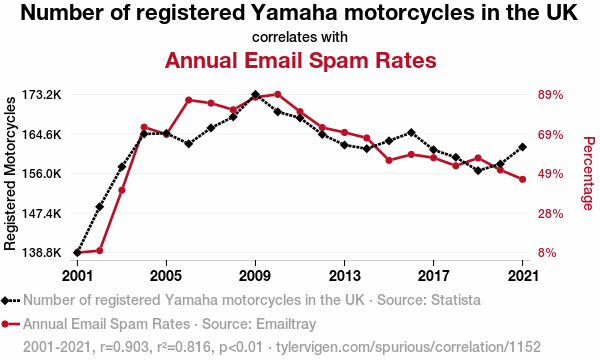
\includegraphics[width=0.8\linewidth]{figures/1152_number-of-registered-yamaha-motorcycles-in-the-uk_correlates-with_annual-email-spam-rates.png}
%     \end{figure}
% \end{frame}


% \begin{frame}{Correlação não implica causalidade}
%     \begin{figure}
%         \centering
%         
\includegraphics[width=0.8\linewidth]{figures/2011_masters-degrees-awarded-in-engineering-technologies_correlates-with_hydopower-energy-generated-in-vietnam.png}
%     \end{figure}
% \end{frame}


% \begin{frame}{Correlação não implica causalidade}
%     \begin{figure}
%         \centering
%         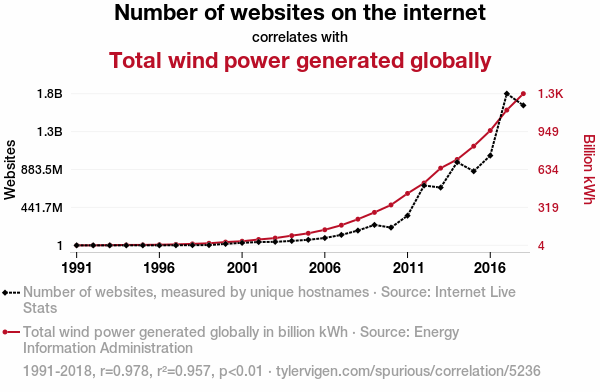
\includegraphics[width=0.8\linewidth]{figures/5236_number-of-websites-on-the-internet_correlates-with_total-wind-power-generated-globally.png}
%     \end{figure}
% \end{frame}

% \begin{frame}{Fim!}
%     Chegamos ao fim da primeira parte da matéria de estatística! 

%     \pause

%     \vspace{5px}

%     Antes de passarmos para a Probabilidade, vamos falar sobre os seguintes pontos:

%     \begin{itemize}
%         \item Como usar o Quarto. 
%         \item Lacunas do R (salvar DataFrame, filtrar DataFrame, valores únicos e obter dimensões do dataframe )
%         \item Explicação do trabalho. 
%     \end{itemize}
% \end{frame}

%\section{Introdução à Probabilidade}

\begin{frame}{Uma breve história da Probabilidade}
    \begin{itemize}
        \item O surgimento da Probabilidade está diretamente ligada ao estudo de jogos de azar. 
        \pause 
        \item A Probabilidade, conforme estudamos hoje, surge em 1654 através de correspondências entre Pierre de Fermat e Blaise pascal acerca do \textbf{Problema dos Pontos} . 
        \pause

        \item Observação: O problema já havia sido proposto, aproximadamente, 100 anos antes por Luca Pacioli (Considerado o pai da contabilidade). 
    \end{itemize}
\end{frame}

\begin{frame}{O Problema dos Pontos}
    Vamos voltar para 1654. 
    \pause
    Vamos jogar o seguinte jogo:

    \textbf{Regras do Jogo:}
    \begin{itemize}
        \item O jogo tem exatamente dois jogadores. 
        \pause
        \item Cada jogador escolhe uma face de uma moeda (Cara ou Coroa).
        \pause
        \item Cada jogador aposta um valor (Exemplo: R\$ 25,00).
        \pause
        \item A cada rodada a moeda é lançada e é anotado o resultado, somando 1 ponto para o jogador que escolheu o resultado obtido.
        \pause
        \item Vence quem obtiver o total de 3 pontos. Levando o prêmio (Nesse caso, R\$ 50,00)
    \end{itemize}
\pause
    \textcolor{red}{Pergunta:} Esse jogo é justo?
\end{frame}

\begin{frame}{Jogando o jogo}
    \textbf{Vamos jogar o jogo!}
    
    \pause

    \textbf{Uma chuva de meteoros cai na UFRJ}
    \begin{figure}
        \centering
        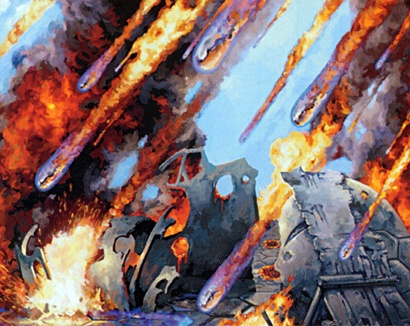
\includegraphics[width=0.5\linewidth]{figures/molten_rain.jpg}
    \end{figure}
    \pause
    Cada jogador está exatamente com dois pontos, como dividir o prêmio?
\end{frame}

\begin{frame}{OJogando o jogo, novamente}
    \textbf{Vamos jogar o jogo de novo!}

    \pause

    \textbf{Uma chuva de meteoros cai na UFRJ}
    \begin{figure}
        \centering
        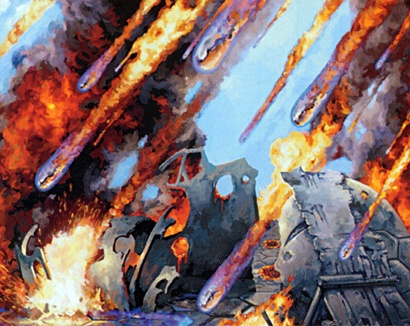
\includegraphics[width=0.5\linewidth]{figures/molten_rain.jpg}
    \end{figure}
    \pause
    Nesse caso, um jogador está com dois pontos e o outro com um ponto, como dividir o prêmio?
\end{frame}

\begin{frame}{O Problema dos Pontos}
    \begin{itemize}
        \item Esse problema ficou conhecido como problema dos pontos. 
        \pause
        \item Pascal e Fermat propõem uma solução para o problema envolvendo probabilidades. 
        \pause
        \item Recomendação de leitura que apresenta as correspondências e realiza comentários:  \href{https://archive.org/details/unfinishedgamepa0000devl}{The Unfinished Game} 
    \end{itemize}
\end{frame}

\begin{frame}{Como começar pelo começo se as coisas acontecem antes de acontecer?}
   \begin{itemize}
    \item De fato, a Probabilidade não começa em 1654, mas sim muito antes, talvez $2.000$ ou $600$ anos antes de cristo. 
    \pause
    \item Mas essa é uma história longa e não será abordada em nossa disciplina. 
   \end{itemize} 
\end{frame}

\begin{frame}{O que significa a probabilidade de algo acontecer?}
    Vamos considerar a seguinte afirmação:

    \begin{itemize}
        \item A probabilidade de chover amanhã é 30\%
    \end{itemize}

    \pause

    O que de fato essa informação nos diz?

\end{frame}

\begin{frame}{O mundo é realmente aleatório?}

    \begin{itemize}
        \item  As coisas realmente acontecem aleatoriamente no mundo em que vivemos?
        \pause
        \item  A aleatoriadade realmente existe?
        \pause
        \item O que é a aleatóriedade?
    \end{itemize} 
\end{frame}

\begin{frame}{Breve comentário sobre aleatoriedade e Teoria do Caos}
    \textbf{Filme: De caso com o acaso (1998)}
    \begin{figure}
        \centering
        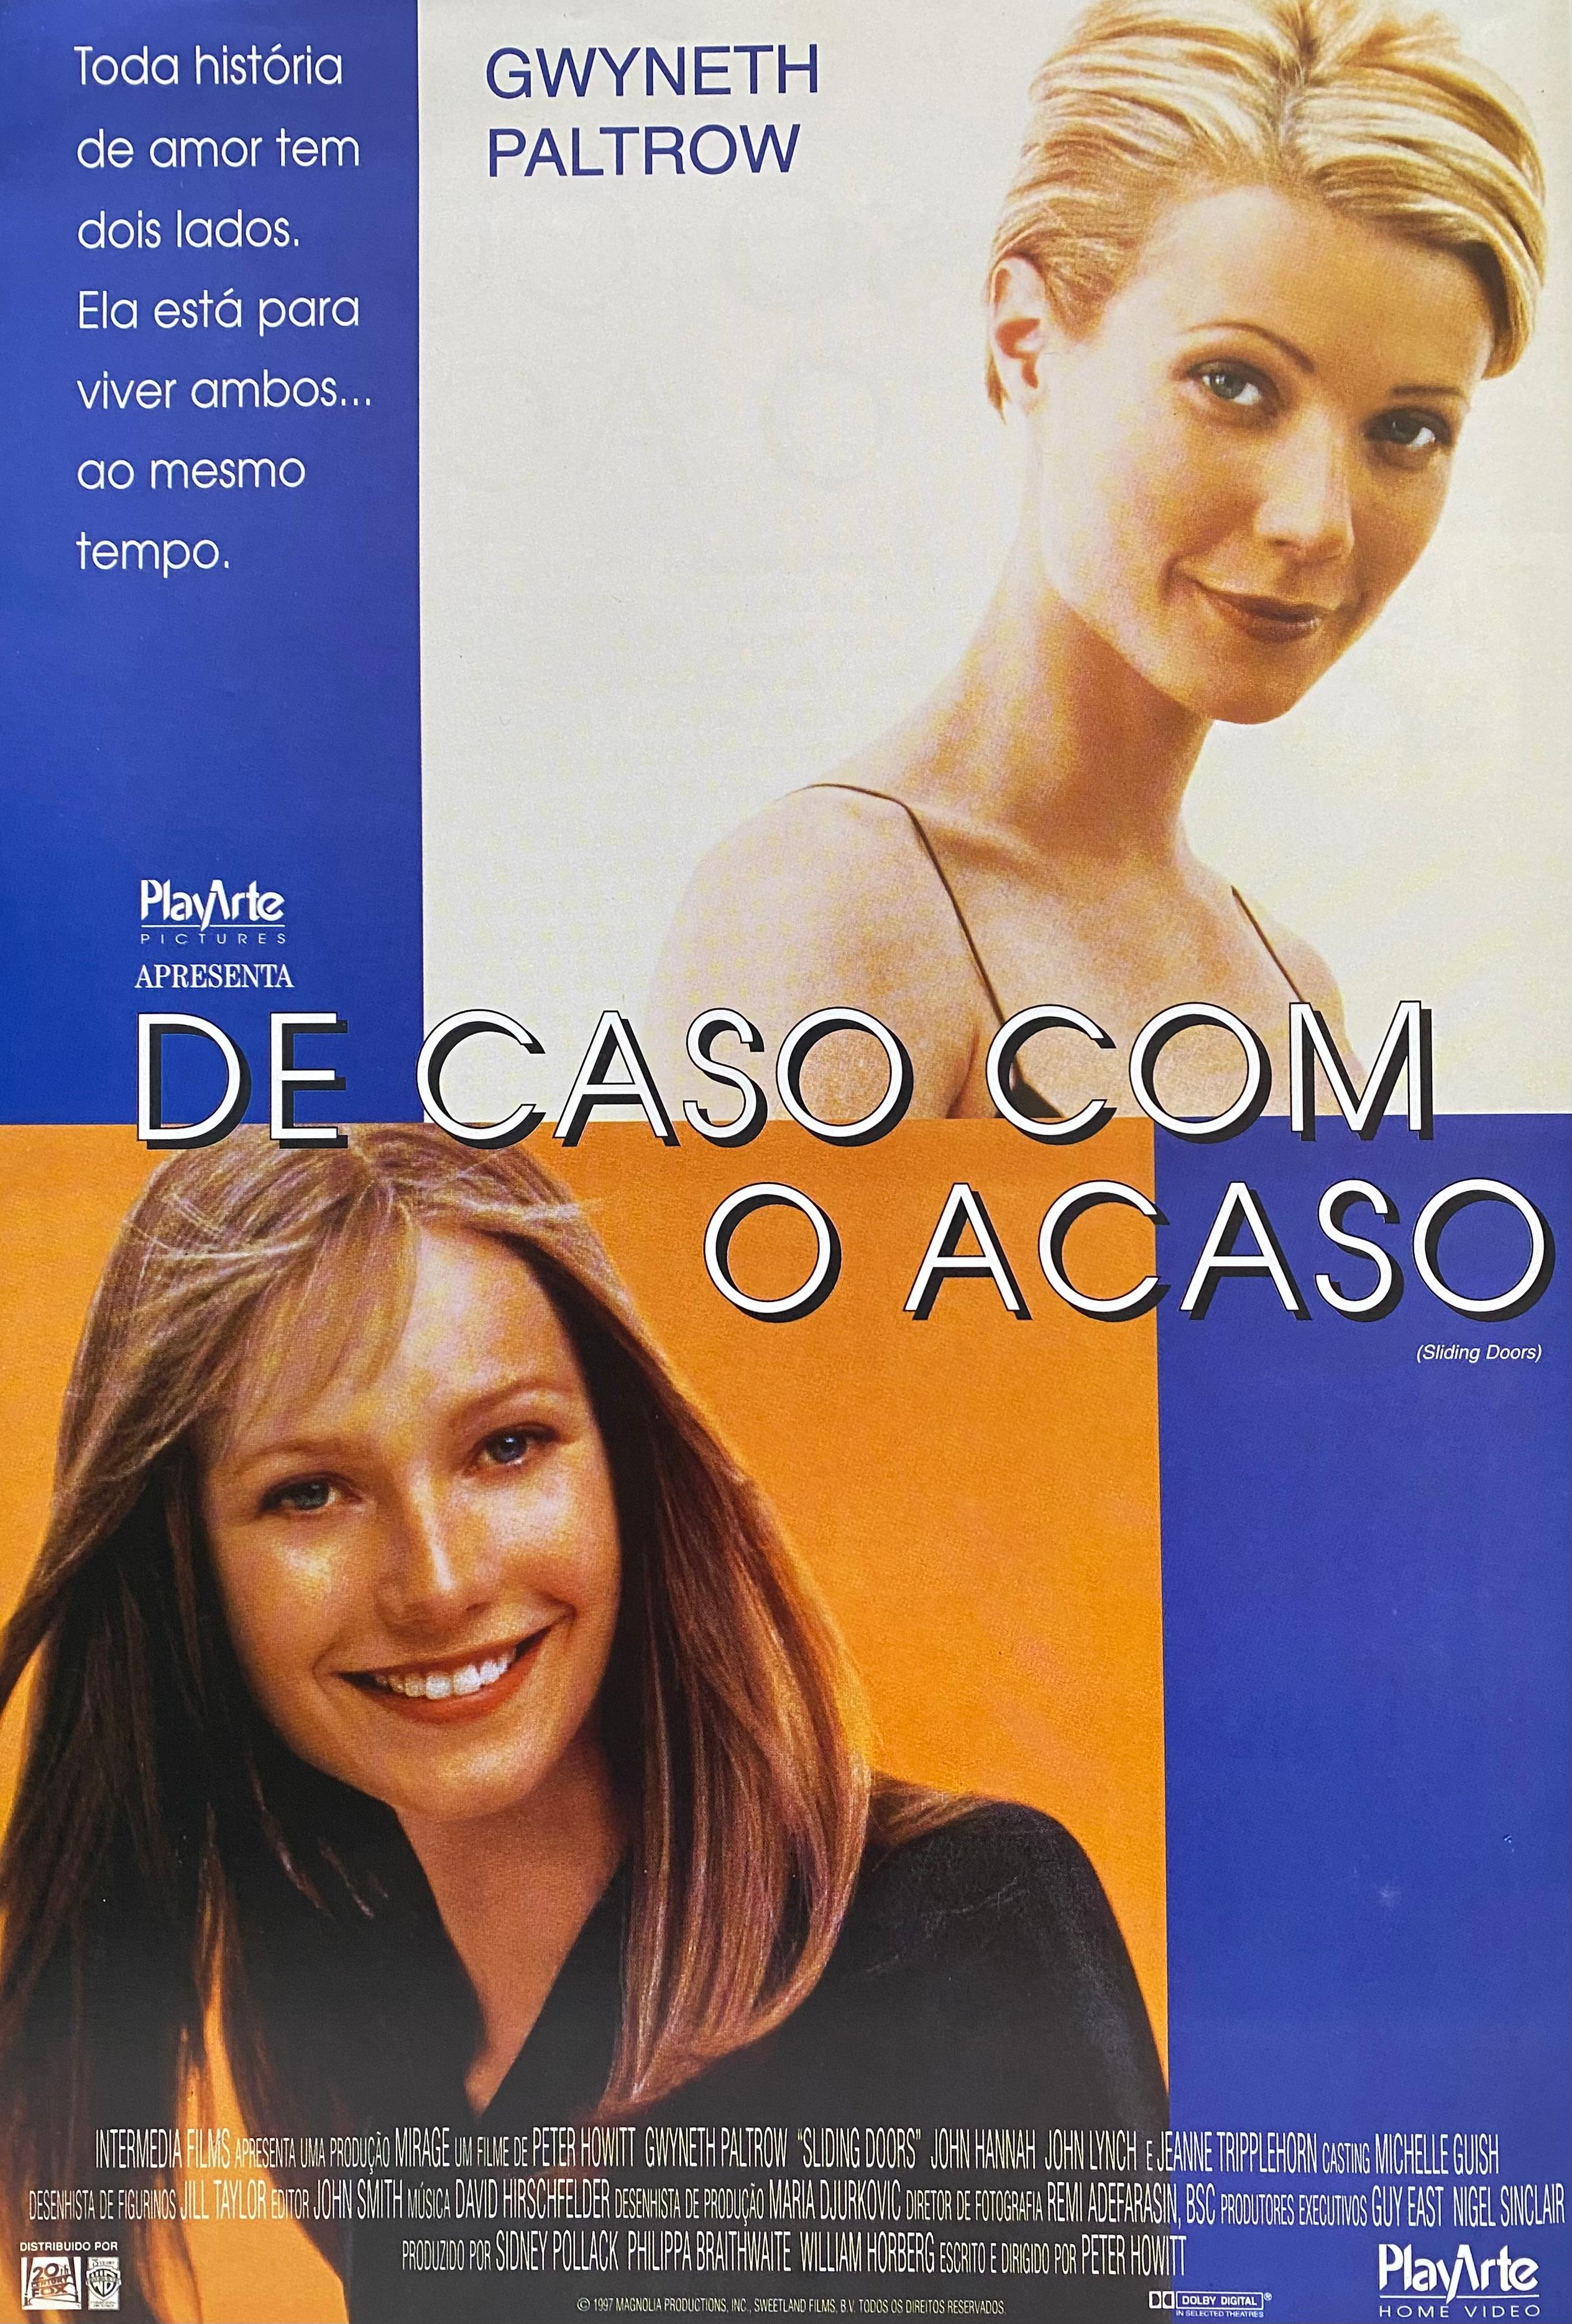
\includegraphics[width=0.4\linewidth]{figures/filme_sliding_doors.jpg}
    \end{figure}
\end{frame}

\begin{frame}
    \begin{itemize}
        \item Apesar disso, será que existe alguma espécie de ordem no caos?
    \end{itemize}

    Vamos jogar um jogo!
\end{frame}

\begin{frame}{Interpretações da Probabilidade}
   \begin{itemize}
    \item Intepretação Clássica: A probabilidade nada mais é que uma simples fração, onde o numerador é o número de casos favoráveis e o denominador é o número de todos os casos possíveis.
    \item Interpretação Frequentista: A probabilidade de um evento ocorrer é igual a frequência observada na qual ele ocorre. 
    \item Intepretação Lógica: Probabilidade como a relação entre proposições. 
    \item Interpretação Subjetivista (Bayesiana). Probabilidade não existe. \pause Exceto na mente de cada um.  
   \end{itemize} 
\end{frame}


\begin{frame}{Experimentos Aleatórios}

\begin{exemplo}
    \begin{enumerate}
        \item Jogar um dado e observar a face superior.
        \item Lançar uma moeda quatro vezes e contar o número de caras.
        \item Em uma linha de produção, fabrica-se peças em série e conte-se o número de peças defeituosas produzidas em um período de 24 horas.
        \item Uma lâmpada é fabricada. Em seguida é ensaiada quanto à duração da vida, pela colocação em um soquete e anotação do tempo decorrido (em horas) até queimar.
        \item Peças são fabricadas até que 10 peças perfeitas sejam produzidas. O número total de peças fabricadas é contado.
    \end{enumerate}
\end{exemplo}
\end{frame}

\begin{frame}{Espaço amostral}
    O espaço amostral, denotado pela letra grega $\Omega$, é definido como o conjunto de todos os possíveis resultados de um experimento. Relacionando com os experimentos anteriores, temos:
    \begin{exemplo}
        \begin{enumerate}
            \item $\Omega =\{1, 2, 3, 4, 5, 6\}$
            \item  $\Omega =\{0, 1, 2, 3, 4\}$
            \item $\Omega =\{0, 1, 2, 3 , \dots, n\}$ onde $n$ é o número máximo que pode ser produzido em 24 horas.
            \item $\{t : t \geq 0\}$
            \item $\{10, 11, 12, \dots\}$
        \end{enumerate}
    \end{exemplo}
\textcolor{red}{Importante}:O espaço amostral está sempre relacionado ao experimento
\end{frame}

\begin{frame}{Espaço amostral}
    \textbf{Qual é o espaço amostral do experimento do lançamento de uma moeda?}

    \begin{itemize}
        \item Vídeo: Lançamento de uma moeda.
    \end{itemize}
\end{frame}
\begin{frame}{Espaço amostral}
    \begin{exemplo}
        Uma caixa contém 3 bolas de gude: 1 vermelha, 1 verde e uma azul. Considere um experimento que consiste em retirar uma bola de gude da caixa, colocada de volta, em seguida outra bola é retirada. Descreva o espaço amostral.
    \end{exemplo}
\end{frame}
\begin{frame}{Eventos}

Um evento é simplesmente um subconjunto de um espaço amostral. Note que o próprio $\Omega$ é um evento. Relacionando com os espaços amostrais construídos anteriormente:

\begin{exemplo}
    \begin{enumerate}
        \item Um número par ocorre, isto é, $A_1= \{2,4,6\}$
        \pause
        \item $\{2\}$; isto é, duas caras ocorrem
        \pause
        \item $\{0\}$; isto é, todas as peças são perfeitas.
        \pause
        \item $\{t : t < 3\}$; isto é, a lâmpada queima em menos de 3 horas.
        \pause
        \item $\{0\}$; isto é, nenhuma peça defeitusosa é fabricada. 
    \end{enumerate}
\end{exemplo}
    
\end{frame}

\begin{frame}{Operações envolvendo eventos}
    Assim como vimos anteriormente, eventos são conjuntos, logo, tudo que vimos de teoria dos conjuntos pode ser também aplicado para eventos. Nesse sentido, definimos as seguintes operações:
    \begin{enumerate}[a)] % a), b), c), ...
        \item Se $A$ e $B$ forem eventos, $A \cup B$ será o evento que ocorrerá se, e somente se, $A$ ou $B$ (ou ambos) ocorrerem.
        \pause
        \item Se $A$ e $B$ forem eventos, $A \cap B$ será o evento que ocorrerá se, e somente se, $A$ e $B$ ocorrerem.
        \pause
        \item Se $A$ for um evento, $A^c$ será o evento que ocorrerá se, e somente se, não ocorrer A.
        \pause
        \item Se $A_1, \dots, A_n$ for qualquer coleção finita de eventos, então $\bigcup_{i=1}^n A_i$ será o evento que ocorrerá se, e somente se, ao menos um dos eventos $A_i$ ocorrer. 
        \pause
        \item Se $A_1, \dots, A_n$ for qualquer coleção finita de eventos, então $\bigcap{i=1}^n A_i$ será o evento que ocorrerá se, e somente se, todos os eventos $A_i$ ocorrer. 
    \end{enumerate}
\end{frame}

\begin{frame}{Eventos mutuamente excludentes}

Dois eventos, A e B, são denominados mutuamente excludentes se eles não puderem ocorrer juntos. Isso significa dizer que $A\cap B = \emptyset$.

\end{frame}

\begin{frame}{Noção primitiva de probabilidade}

Assumindo que todos os elementos do espaço amostral são equiprováveis, de forma ingênua, definidos a probabilidade de um evento $A$ ocorrer da seguinte forma:

$$\mathds{P}(A) = \dfrac{\text{número de elementos em A}}{\text{número de elementos em }  \Omega} $$

\pause
\begin{exemplo}
    Uma moeda honesta é lançada duas vezes, qual a probabilidade de sair duas caras?
\end{exemplo}

\pause 
\begin{exemplo}
    Um dado de seis faces é lançado. Qual a probabilidade de sair um número maior do que 4? 
\end{exemplo}

\end{frame}

\begin{frame}
    \begin{exemplo}
        Ao lançarmos dois dados de seis faces, qual a probabilidade da soma dos dois ser igual a sete?
            
        \end{exemplo}
\end{frame}

\begin{frame}{Probabilidade como função}

A noção primitiva de probabilidade nos diz como calcular probabilidades, mas não o que de fato é probabilidade. 

\begin{definicao}
    Probabilidade, denotada por $\mathds{P}$ é uma função que toma um evento $A \subset \Omega$ como entrada e retorna $\mathds{P}(A) \in [0,1]$ como saída. Essa função deve satisfazer as seguintes propriedades:

    \begin{enumerate}
        \item $\mathds{P}(\Omega) = 1$
        \item Para todo evento $A$, $\mathds{P}(A) \geq 0$
        \item Se $A$ e $B$ forem eventos mutuamente excludentes, então $\mathds{P}(A \cup B) = \mathds{P}(A) + \mathds{P}(B)$
        \item Seja $A_1, A_2, \dots, A_n$ uma sequência de eventos mutuamente exclusivos dois a dois, então $\mathds{P}(\bigcup_{i=1}^n A_i) = \sum_{i=1}^{n} \mathds{P}(A_i)$
    \end{enumerate}

\end{definicao}
    
\end{frame}

\begin{frame}{Probabilidade - Propriedades}

A partir das propriedades definidas no slide anterior, podemos derivar outras propriedades. Sejam $A$ e $B$  eventos, logo temos que:
\begin{enumerate}
    \item $\mathds{P}(\emptyset) = 0$
    \pause
    \item $\mathds{P}(A^c) = 1 - \mathds{P}(A)$
    \pause
    \item Se $A \subset B$ então $\mathds{P}(A) \leq \mathds{P}(B)$
    \pause
    \item $0 \leq \mathds{P} \leq 1$
    \pause
    \item $\mathds{P}(A \cap B^c) = \mathds{P}(A) - \mathds{P}(A \cap B)$
    \pause
    \item $\mathds{P}(A \cup B) = \mathds{P}(A) + \mathds{P}(B) - \mathds{P}(A \cap B)$ *
\end{enumerate}
    * Principio da inclusão-exclusão
\end{frame}

\begin{frame}{Probabilidade}
    \begin{exemplo}
        De uma dada população, 42\% são ruivos, 35\% tem olhos azuis e 20\% são ruivos de olhos azuis. Escolhendo ao acaso uma pessoa dessa população, qual a probabilidade de
        \begin{enumerate}[a)] % a), b), c), ..
            \item Ser ruivo ou ter olhos azuis?
            \item Não ser ruivo e ter olhos azuis?
            \item Ser ruivo mas não ter olhos azuis?
        \end{enumerate}
    \end{exemplo}

\end{frame}

\begin{frame}{Probabilidade}
    \begin{exemplo}
        Um lote contém peças pesando 5, 10, 15, 20, 25 gramas. Admitamos que ao menos duas peças de cada peso sejam encontradas no lote. Duas peças são retiradas do lote. Sejam $X$ o peso da primeira peça escolhida e $Y$ o peso da segunda. 
        \begin{enumerate}[a)] % a), b), c), ..
            \item Determine o espaço amostral desse experimento.
            \item Determine a probabilidade de $X$ ser igual a Y.
            \item Determine a probabilidade de $Y$ ser maior do que $X$.
            \item Determine a probabilidade da primeira peça pesar 10 gramas a menos que a segunda peça.
        \end{enumerate}
    \end{exemplo}
\end{frame}

\begin{frame}{Probabilidade}
    Um professor de uma disciplina decide montar os grupos de um trabalho da seguinte forma:
    \begin{enumerate}
        \item Serão definidos 8 temas.
        \item Serão definidos dois grupos para cada tema. 
        \item Cada grupo deve conter exatamente 2 alunos. 
        \item Os alunos devem manifestar interesse no tema, respeitando o limite máximo de 4 pessoas por tema. Sendo a formação do grupo definida de forma aleatória pelo professor. 
    \end{enumerate}

    \pause

    Suponha que Ana e Marcos desejam fazer o trabalho em dupla e, portanto, se inscreveram no mesmo tema. Qual a probabilidade de que eles terminem no mesmo grupo?
\end{frame}

\begin{frame}{Probabilidade condicional}
    \begin{itemize}
        \item  A probabilidade de um evento ocorrer pode ser modificada ao descobrirmos novas informações que o afete.
        \pause 
        \item Considere o experimento do lançamento de dois dados. Qual a probabilidade da soma dos resultados do lançamento dos dados dar 6 ?
        \pause
        \item Digamos que o primeiro dado apresentou o número 3. Qual a probabilidade da soma dos resultados ser igual a 6?
        \pause
        \item Digamos que um dos dados apresentou o número 3. Qual a probabilidade da soma dos valores ser um número par?
    \end{itemize}
   

\end{frame}

\begin{frame}{Probabilidade condicional}

O problema proposto anteriormente é chamado de probabilidade condicional.

\begin{definicao}
    Sejam A e B dois eventos com $\mathds{P}(B>0)$. Dado que sabemos que B ocorreu, a probabilidade do evento A ocorrer pode ser definida como:

    $$\mathds{P}(A|B) = \dfrac{\mathds{P}(A \cap B)}{\mathds{P}(B)}$$
\end{definicao}
\end{frame}

\begin{frame}{Probabilidade condicional}
    Uma editora lançou 360 livros e pode dividi-los entre ficção e não-ficção ou entre nacionais e internacionais segundo a tabela a seguir:
    
    \begin{table}[H]
        \centering
        \begin{tabular}{|c|c|c|c|}
        \hline
        \textbf{Origem \textbackslash{} Estilo} & \textbf{Ficção} & \textbf{Não-ficção} & \textbf{Total} \\
        \hline
        Nacional     & 90  & 70  & 160 \\
        \hline
        Internacional & 120 & 80  & 200 \\
        \hline
        \textbf{Total}       & 210 & 150 & 360 \\
        \hline
        \end{tabular}
        \caption{Distribuição de livros por origem e estilo}
        \end{table}
        
        \pause

        \begin{itemize}
            \item Um livro é escolhido. Qual a probabilidade do livro escolhido ser nacional dado que é um livro não-ficcional. 
        \end{itemize}
\end{frame}

\begin{frame}{Regra da multiplicação}
 Sejam $A$ e $B$ dois eventos com $\mathds{P}(B)>0$. Então vale:
 $$\mathds{P}(A \cap B) = \mathds{P}(A | B) \mathds{P}(B) = \mathds{P}(B | A) \mathds{P}(A)$$
\end{frame}

\begin{frame}
\begin{exemplo}
    Uma urna contém 4 bolinhas amarelas e 2 bolinhas verdes. Um
experimento consiste em retirar uma bolinha, verificar sua cor e retirar uma
segunda bolinha sem reposição. Calcule a probabilidade associada a cada re-
sultado desse experimento.
\end{exemplo}

\textbf{Observação:} Resolva usando a regra da multiplicação e o diagrama de árvore. 
\end{frame}

\begin{frame}{Regra da multiplicação}
    Podemos generalizar a regra da multiplicação para mais de 2 eventos:

    \pause

Sejam $A_1, A_2, \dots , A_n$ eventos num mesmo espaço amostral. Se
    $P(\cap_{i=1}^{n-1}A_i) > 0$, então:

    $$\mathds{P}(\cap_{i=1}^n A_i) = \mathds{P}(A_1)\mathds{P}(A_2|A_1) \cdot \dots \cdot \mathds{P}(A_n|A_i, \dots, A_{n-1} )$$

\end{frame}
\begin{frame}{Particionamento do espaço amostral}
Uma técnica que nos será últil a partir de agora é particionar (dividir) o espaço amostral em eventos \textbf{mutuamente excludentes} de tal forma que a união deles
seja o próprio espaço amostral. 
\end{frame}

\begin{frame}{Particionamento do espaço amostral}
    \begin{definicao}
        Sejam A e B dois eventos em um mesmo espaço amostral:
        $$\mathds{P}(A) = \mathds{P}(A|B)\mathds{P}(B) + \mathds{P}(A|B^c)\mathds{P}(B^c)$$
    \end{definicao}
\end{frame}

\begin{frame}{Particionamento do espaço amostral}
    \begin{exemplo}[1]
        Em certo hospital especializado em doenças respiratórias, 75\% dos pacientes são fumantes ou ex-fumantes e são indicados pelo código F, enquanto pacientes que nunca fumaram são indicados pelo código NF. Cerca de 60\% dos pacientes do grupo F precisam de internação, enquanto apenas 20\% dos não-fumantes  são internados. Se escolhermos ao acaso um paciente que acabou de entrar no hospital, qual a probabilidade dele precisar de internação?
    \end{exemplo}
\end{frame}

\begin{frame}{Particionamento do espaço amostral}
    Podemos generalizar essa noção para $n$ eventos através do Teorema abaixo, conhecido como \textbf{Lei da Probabilidade Total}
    Seja $\{B_1, \dots, B_n\}$ uma partição do espaço amostral $\Omega$, onde, $\Omega=\bigcup_{i=1}^n B_i$, $\mathds{P}(B_i)>0$ e $\{B_1, \dots, B_n\}$ disjuntos dois a dois. Se $A$ é um evento qualquer em $\Omega$, vale:

    $$\mathds{P}(A) = \sum_{i=1}^n \mathds{P}(A|B_i)\mathds{P}(B_i)$$
\end{frame}

\begin{frame}{Particionamento do espaço amostral}
\begin{exemplo}[2]
    Suponha que um fabricante de sorvetes recebe 20\% de todo o leite que utiliza em uma fazenda $F_1$, 30\% de uma outra fazenda $F_2$ e 50\% de $F_3$. Um orgão de fiscalização inspecionou as fazendas de surpresa e observou que 20\% do leite produzido por $F_1$ estava adulterado por adição de água, enquanto para $F_2$ e $F_3$, essa proporção era de 5\% e 2\%, respectivamente. Na indústria de sorvetes, os galões de leite são armazenados em um refrigerador sem identificação das fazendas. 

    \begin{itemize}
        \item Qual a probabilidade do leite estar adulterado?
    \end{itemize}
\end{exemplo}
\end{frame}

\begin{frame}{Teorema de Bayes}

    Sejam $A$ e $B$ dois eventos e $\mathds{P}(B)>0$. Então vale:
    
$$\mathds{P}(A|B) = \dfrac{\mathds{P}(B | A)\mathds{P}(A)}{\mathds{P}(B)}$$
    
\end{frame}

\begin{frame}{Teorema de Bayes}
        \begin{exemplo}[3]
        Em dado aeroporto, sabe-se que 90\% dos pousos atrasam em dias de chuva e 15\% nos dias que não chove. Seu amigo tem um voo com destino a esse aeroporto e a previsão de tempo disse que com probabilidade 0,4 estaria chovendo na região. Dado que o pouso está atrasado, qual a probabilidade de estar chovendo na região do aeroporto?
    \end{exemplo}
\end{frame}
\begin{frame}{Teorema de Bayes}
    \begin{exemplo}[4]
        Suponha que um fabricante de sorvetes recebe 20\% de todo o leite que utiliza em uma fazenda $F_1$, 30\% de uma outra fazenda $F_2$ e 50\% de $F_3$. Um orgão de fiscalização inspecionou as fazendas de surpresa e observou que 20\% do leite produzido por $F_1$ estava adulterado por adição de água, enquanto para $F_2$ e $F_3$, essa proporção era de 5\% e 2\%, respectivamente. Na indústria de sorvetes, os galões de leite são armazenados em um refrigerador sem identificação das fazendas. 

        \begin{itemize}
            \item Qual é a probabilidade do leite ser proveniente da fazenda $F_1$ dado que o leite está adulterado?
        \end{itemize}
    \end{exemplo}

    
\end{frame}

\begin{frame}{Teorema de Bayes}
\begin{exemplo}[5]
        Uma clínica envia amostras de uma certa substância para 3 laboratórios de análises A, B e C nas seguintes proporções 0,2; 0,3; 0,5 respectivamente. A probabilidade de cada um dos laboratórios elaborar uma análise errada é de $\dfrac{1}{2}, \dfrac{1}{3}, \dfrac{1}{6}$ respectivamente. Baseado nessas informações, pergunta-se:

    \begin{itemize}
        \item Qual é a probabilidade de um exame executado dar errado?
        \item Uma análise resultou errada, qual a probabilidade de ter sido feita pelo laboratório A? Pelo B? Pelo C?
    \end{itemize}
\end{exemplo}

\end{frame}

\begin{frame}{Teorema de Bayes}
\begin{exemplo}[6]
        Pelo fato de um novo procedimento médico ter se mostrado efetivo na detecção prévia de uma doença, propôs-se um rastreamento médico da população. A probabilidade do teste identificar corretamente alguém com a doença, dando positivo, é de 0,99 e a probabilidade do teste identificar corretamente alguém sem a doença, dando negativo, é de 0,95. A incidência da doença na população é 0,0001. Você fez o teste e o resultado foi positivo. Qual a probabilidade de você ter a doença?
\end{exemplo}

\end{frame}

\begin{frame}{Independência}
    Dizemos que dois eventos A e B definidos em um mesmo espaço amostral são independentes se:
    $$\mathds{P}(A\cap B) = \mathds{P}(A) \mathds{P}(B)$$
\end{frame}

\begin{frame}{Independência}
\begin{exemplo}[7]
    Suponha que a probabilidade de uma pessoa ser do tipo sanguíneo O é 0,45, ser A é 0,42 e ser B é 0,10. Suponha ainda que a probabilidade de $Rh^+$ é se 0,90 e que o fator independe do tipo sanguíneo. Nestas condições, qual a probabilidade de uma pessoa tomada ao acaso da população ser:

    \begin{itemize}
        \item O e $Rh^+$
        \item AB e $RH^-$
    \end{itemize}
\end{exemplo}
    
\end{frame}

\begin{frame}{Independência}

\begin{exemplo}
    Ao lançarmos dois dados de seis faces, considere os eventos:
    \begin{itemize}
        \item A: O resultado do primeiro é 4
        \item B: A soma dos dois resultados é 7
    \end{itemize}

    A e B são independentes?
\end{exemplo}
    
\end{frame}

\begin{frame}{Variáveis aleatórias}
    Em muitos experimentos é útil trabalhar com uma "variável resumo".

    \begin{exemplo}[8]
        Numa pesquisa de opinião, decidimos perguntar a 20 pessoas se elas concordam ou discordam sobre determinado assunto. Nessa pesquisa, anotaremos o valor 1 se a pessoa concorda e 0 se a pessoa discorda.

        \begin{itemize}
            \item Observe que o tamanho do espaço amostral desse experimento contém $2^{20}=1048576$ elementos.
            \item Podemos estar interessados em características específicas em relação aos elementos do espaço amostral. 
        \end{itemize}
    \end{exemplo}
\end{frame}

\begin{frame}{Variáveis aleatórias}

\begin{definicao}
    Uma variável aleatória nada mais é que uma função que toma como entrada elementos do espaço amostral e gera como saída um número real
\end{definicao}

\begin{itemize}
    \item Variáveis aleatórias serão denotadas em geral por letras maiúsculas do final do alfabeto: $W, X, Y, Z$
    \pause
    \item Denotaremos por $\Omega_X$ o conjunto de possíveis valores assumidos pela Variável Aleatória $X$.
    \pause
    \item \textcolor{red}{Atenção}: Note que $X$ pode ser a função identidade, $\Omega_X$ é igual a $\Omega$.
\end{itemize}
\begin{figure}
    \centering
    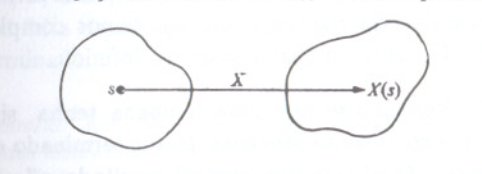
\includegraphics[width=0.5\linewidth]{figures/variavel_aleatoria.png}
    \label{fig:enter-label}
\end{figure}

\end{frame}
\begin{frame}{Variáveis aleatórias}
    \begin{exemplo}[9]
        Considere o experimento do lançamento de duas moedas. Nesse caso temos:
        $$\Omega = \{(Cara, Cara), (Coroa, Coroa), (Cara, Coroa), (Coroa, Cara)\}$$

        Definamos a variável aleatória $X:$Número de caras obtidas nas duas moedas. Dessa forma temos, $X((Cara, Cara)) = 2$, $X((Cara, Coroa)) = 1$,  $X((Coroa, Cara)) = 1$, $X((Coroa, Coroa)) = 0$
    \end{exemplo}

\end{frame}

\begin{frame}{Variáveis aleatórias discretas}
    \begin{definicao}
        Uma variável aleatória discreta é aquela que pode tomar apenas um número contável de valores, tais como $0,1,2,3,4, \dots$. Denotaremos por $\Omega_X$ o conjunto de possíveis valores que essa variável pode assumir.

        \begin{itemize}
            \item Variáveis aleatórias discretas geralmente estão relacionadas à contagem. 
        \end{itemize}
    \end{definicao}
\end{frame}

\begin{frame}{Variáveis aleatórias discretas}
\begin{exemplo}[10]
    Se lançamos três dados de seis faces podemos definir, entre outras, as seguintes variáveis aleatórias discretas:
    \begin{itemize}
        \item X: A soma dos resultados:
            $$\Omega_X = \{3,4,5,\dots, 16,17,18\}$$
        \item: X: O produto dos dois primeiros resultados:
            $$\Omega_X = \{1, 2, 3, 4, 5, 6, 8, 9, 10, 12, 15, 16, 18, 20, 24, 25, 30, 36\}$$
            \item X: O máximo entre os resultados:
            $$\Omega_X = \{1,2,3,4,5,6\}$$
            \item X: O mínimo entre os resultados:
            $$\Omega_X =  \{1,2,3,4,5,6\}$$
            \item X: O número de vezes em que apareceu o resultado 6:
            $$\Omega_X =  \{1,2,3\}$$
    \end{itemize}
\end{exemplo}
\end{frame}

\begin{frame}{Variáveis aleatórias discretas}
    \begin{exemplo}
        \begin{figure}
            \centering
            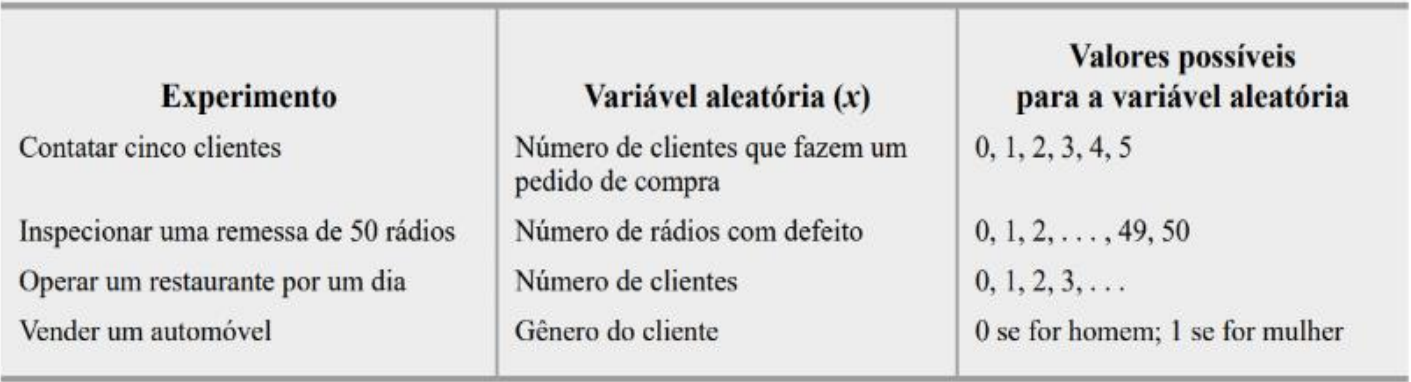
\includegraphics[width=1\linewidth]{figures/tab_exemplo_va_discreta.png}
        \end{figure}
    \end{exemplo}
\end{frame}

\begin{frame}{Distribuição de uma variável aleatória discreta}
    A função de probabilidade de uma variável aleatória discreta é uma lista com as probabilidades associadas a cada possível valor que a variável assume. Também é chamada de função massa de probabilidade. Seja $X$ uma variável aleatória que assume os valores $x_1, x_2, \dots, x_n$, utilizaremos a seguinte notação para representar essa função:

    $$p(x_i) = \mathds{P}(X=x_i)$$

    Essa função deve satisfazer as seguintes propriedades:

\begin{itemize}
    \item $p_X(x_i) \geq 0$ para todo $i$,
    \item $\sum_{i=1}^{n} p_X(x_i) = 1$
\end{itemize}
\end{frame}

\begin{frame}{Distribuição de uma variável aleatória discreta}
    Considere o experimento de lançar uma moeda honesta para o ar 3 vezes e anotar a sequência dos resultados

    \begin{itemize}
        \item Qual o espaço amostral desse experimento?
    \end{itemize}
\end{frame}

\begin{frame}{Distribuição de uma variável aleatória discreta}
    Considere o experimento de lançar uma moeda honesta para o ar 3 vezes e anotar a sequência dos resultados

    \begin{itemize}
        \item Qual o espaço amostral desse experimento?
        \item Definamos a variável aleatória Y: Número de caras obtidas, qual a função de probabilidade associada a essa variável?
    \end{itemize}

\end{frame}

\begin{frame}{Distribuição de uma variável aleatória discreta}

\begin{exemplo}[11]
     Em um processo de fabricação de semicondutores, três pastilhas de um lote são testadas. Cada pastilha é classificada como "passa" ou "falha". Suponha que a probabilidade de uma pastilha passar no teste seja 0,8 e que as pastilhas sejam independentes. Seja a variável resposta $X$ definida como o número de pastilhas de um lote que passa no teste. 

     \begin{itemize}
         \item Defina o espaço amostral desse experimento
         \item Determine a função de probabilidade de $X$.
     \end{itemize}
     
\end{exemplo}
   
\end{frame}
\begin{frame}{Função distribuição acumulada}
    \begin{definicao}
        Seja $X$ uma variável aleatória, definiremos sua \textbf{Função distribuição acumulada} da seguinte forma:
        
$$F_X(x) = \mathds{P}(X \leq x)$$
    \end{definicao}
\end{frame}

\begin{frame}{Função distribuição acumulada}
    \begin{exemplo}[12]
        Considere a variável aleatória $X$ que representa o número de pedidos durante o período de 5 minutos em uma empresa de vendas online.

        \begin{figure}
            \centering
            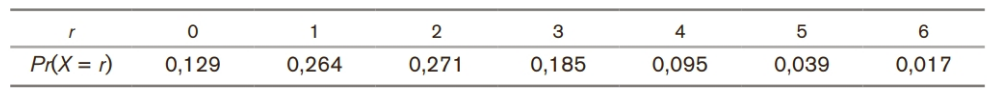
\includegraphics[width=1\linewidth]{figures/exemplo_otite.png}
        \end{figure}
        Nesse caso:
        \pause
        \begin{itemize}
            \item $F_X(-1) = \mathds{P}(X \leq -1) = 0$
            \item $F_X(0) = \mathds{P}(X \leq 0) = \mathds{P}(X=0) = 0,129$
            \item $F_X(1) = \mathds{P}(X \leq 1) = \mathds{P}(X=0) + \mathds{P}(X=1) = 0,129 + 0,264 = 0,393$\\
            \item $F_X(2) = \mathds{P}(X \leq 2) = \mathds{P}(X=0) + \mathds{P}(X=1) + \mathds{P}(X=2) = 0,129 + 0,264 + 0,271 = 0,664 $
        \end{itemize}
    \end{exemplo}
\end{frame}

\begin{frame}{Função distribuição acumulada}
            \begin{itemize}
            \item $F_X(-1) = \mathds{P}(X \leq -1) = 0$
            \item $F_X(0) = \mathds{P}(X \leq 0) = \mathds{P}(X=0) = 0,129$
            \item $F_X(1) = \mathds{P}(X \leq 1) = \mathds{P}(X=0) + \mathds{P}(X=1) = 0,129 + 0,264 = 0,393$\\
            \item $F_X(2) = \mathds{P}(X \leq 2) = \mathds{P}(X=0) + \mathds{P}(X=1) + \mathds{P}(X=2) = 0,129 + 0,264 + 0,271 = 0,664 $
            \item \vdots
            \item $F_X(6) = \mathds{P}(X \leq 6)=1$
        \end{itemize}
\end{frame}

\begin{frame}{Variável aleatória discreta}
\begin{exemplo}[12]
    

    Considere a variável aleatória $X$ possuindo a seguinte função de probabilidade:

    \begin{table}[]
\begin{tabular}{cc}
\hline
x  & $p_X(x)$ \\ \hline
20 & 0,20     \\
25 & 0,15     \\
30 & 0,25     \\
35 & 0,40     \\ \hline
\end{tabular}
\end{table}

\begin{enumerate}
    \item Esta distribuição de probabilidade é valida? Explique.
    \item Qual a probabilidade de $X$ ser igual a 30?
    \item Qual a probabilidade de $X$ ser menor ou igual a 25?
    \item Qual é a probabilidade de $X$ ser maior que 30?
\end{enumerate}
\end{exemplo}
\end{frame}
\begin{frame}
    Imagine o seguinte jogo:
    \begin{itemize}
        \item O jogador aposta $R\$ 10,00$ e escolhe cara ou coroa
        \item Uma moeda honesta é jogado ao ar.
        \item Se a moeda mostrar o resultado cara, então o jogador ganhar  $R\$ 10,00$. Caso contrário, perde os $R\$ 10,00$ apostados. 
    \end{itemize}

    \pause
    Esse jogo é justo?
\end{frame}

\begin{frame}{Esperança Matemática para Variáveis Discretas }
    O valor esperado, média, ou esperança matemática é uma quantidade utilizada como resumo do comportamento de uma V.A. 

    $$\mathbb{E}[X] = \sum_{x_i \in \Omega_X} x_i \mathds{P}(X=x_i)$$
\end{frame}

\begin{frame}{Esperança Matemática para Variáveis Discretas }
    Historicamente, o conceito de esperança foi usado para verificar se jogos eram justos. Entretanto, esse conceito não se restringe apenas à esse campo. 

    \pause

    Vamos verificar se o jogo proposto anteriormente é justo:
    \begin{itemize}
        \item Definamos $X$: ganho obtido no jogo. 
        \pause
        \item $\mathds{E}[X] = 10 \cdot \dfrac{1}{2} -10 \cdot \dfrac{1}{2} = 0 $
        \pause
        \item Portanto, o jogo é justo. 
    \end{itemize}
\end{frame}

\begin{frame}{Esperança Matemática para Variáveis Discretas }
\begin{exemplo}
Um jogo funciona da seguinte forma:
    \begin{itemize}
        \item O jogador deve pagar R\$10,00 para participar do jogo.
        \item Se a soma dos resultados dos dois dados for igual a 10, então o jogador ganha $R\$200,00$
        \item Se a soma dos resultados dos dois dados for igual a 7, então o jogador perde $R\$100,00$
        \item Se a soma dos resultados dos dois dados for um número primo diferente de 7, então o jogador ganha $R\$100,00$
        \item Se a soma dos resultados dos dois dados for um número não-primo diferente de 10, então o jogador perde  $R\$50,00$
    \end{itemize}
    Sabendo disso, defina uma variável aleatória como sendo o ganho (ou perda) obtido pelo jogador, obtenha sua esperança e responda a seguinte pergunta: Esse jogo é justo?
\end{exemplo}    
\end{frame}

\begin{frame}{Esperança Matemática para Variáveis Discretas }
    Vamos jogar outro jogo:
    \begin{itemize}
        \item O jogador deve apostar $x$ reais, com $x > 0$.
        \pause
        \item Uma moeda honesta é jogado ao ar até que saia cara pela primeira vez.
        \pause
        \item O número de jogadas até sair cara (inlcuindo a própria rodada que saiu cara) é denotado por $n$.
        \pause
        \item O jogador ganha $R\$: 2^n$
        \pause
        \item Qual o valor de $x$ para que esse jogo seja justo?
    \end{itemize}
\end{frame}

\begin{frame}{Esperança Matemática para Variáveis Discretas }
    O jogo do slide anterior ficou conhecido como Paradoxo de São Petesburgo. Sua proposição provoca discussões que se estendem até os dias de hoje. 
\end{frame}

\begin{frame}{Esperança Matemática para Variáveis Discretas }
    Vamos sair um pouco do contexto dos jogos. Se eu jogo um dado simétrico de seis faces, 
    definindo $X:$ Resultado apresentado pelo dado. 
\pause
    $$\mathds{E}[X] = \sum_{s=1}^{6} s \cdot \frac{1}{6} = 3,5$$
\pause
Qual o significado do valor $3,5$?
\end{frame}

\begin{frame}{Variância de Variáveis Aleatórias}
    A variância representa o grau de dispersão de uma variável aleatória em relação a sua média ou esperança $\mathbb{E}[X]$. A forma geral para o cálculo é:

    $$Var(X) = \mathbb{E}[(X - \mathbb{E}[X])^2]$$

    Uma forma alternativa de presentar a variância é através da seguinte expressão:

    $$Var(X) = \mathbb{E}[X^2] - \mathbb{E}[X]^2$$

    onde

     $$\mathbb{E}[X^2] = \sum_{x_i \in \Omega_X} x_i^2 \mathds{P}(X=x_i)$$
\end{frame}

\begin{frame}{Exemplos}
\begin{exemplo}
     Considere o experimento de lançar uma moeda honesta para o ar 5 vezes e anotar a sequência dos resultados

    \begin{itemize}
        \item Qual o espaço amostral desse experimento?
        \item Definamos a variável aleatória Y: Número de tentativas até obter a primeira cara, qual a função de probabilidade associada a essa variável?
        \item Calcule o valor esperado da variável Y.
        \item Calcule a variância da variável Y.
    \end{itemize} 
\end{exemplo}
    
\end{frame}

\begin{frame}{Exemplos}
    \begin{exemplo}[11]
     Em um processo de fabricação de semicondutores, três pastilhas de um lote são testadas. Cada pastilha é classificada como "passa" ou "falha". Suponha que a probabilidade de uma pastilha passar no teste seja 0,8 e que as pastilhas sejam independentes. Seja a variável resposta $X$ definida como o número de pastilhas de um lote que passa no teste. 

     \begin{itemize}
         \item Defina o espaço amostral desse experimento
         \item Determine a função de probabilidade de $X$.
         \item Determine o valor esperado de $X$.
         \item Determine a variância de $X$.
     \end{itemize}
     
\end{exemplo}
\end{frame}


\begin{frame}{Outras medidas de dispersão}

Também podemos calcular o desvio padrão de uma variável aleatória. 

$$DP(X) = \sqrt{Var(X)}$$

Além disso, podemos calcular o coeficiente de variação

$$CV = \dfrac{DP(X)}{\mathbb{E}[X]}$$
\end{frame}

\begin{frame}{Propriedades do Valor Esperado e Variância}
    $$\mathbb{E}[aX +b] = a\mathbb{E}[X] + b$$
    $$Var(aX +b) = a^2Var(X)$$

    Sejam $X_1, X_2, \dots, X_n \text{ v.as independentes com } \mathbb{E}[X_i]<\infty$ então:

$$\mathbb{E}[X_1 + X_2 + \dots + X_n] = \mathbb{E}[X_1] + E[X_2] + \dots + \mathbb{E}[X_n]$$
\end{frame}

\begin{frame}{Distribuições de Probabilidade para Variáveis Aleatórias Discretas}
    Algumas variáveis aleatórias aparecem com bastante frequência em situações práticas e justificam um estudo mais aprofundado. Em geral, nesses casos, a \textbf{função de probabilidade} pode ser escrita de maneira mais compacta, isto é, existe uma lei para atribuir probabilidades. 

    As distribuições de probabilidade para variáveis discretas mais importantes são:

    \begin{itemize}
        \item Distribuição de Bernoulli
        \item Distribuição Binomial 
        \item Distribuição de Poisson
        \item Distribuição Geométricas
        \item Distribuição Hipergeométrica
        \item Distribuição Binomial negativa
    \end{itemize}
\end{frame}

\begin{frame}{Distribuição de Bernoulli}

Considere os seguintes experimentos:

\begin{itemize}
    \item Lançamento de uma moeda 
    \item Retirada de uma peça de um conjunto de 10 peças seguido pela verificação se a peça é defeituosa ou não
    \item Pesquisa de opinião se aprova ou não aprova a atual gestão da UFRJ. 
    \item Um aluno realiza uma prova e em seguida verifica se passou ou não. 
    \item Realização de inseminação artificial seguida pela verificação se ocorreu gravidez ou não.
\end{itemize}

    O que esses experimentos tem em comum?

    \pause

    Todos os experimentos acima tem unicamente dois resultados possíveis. Sendo possível criar uma variável aleatória que associe cada resultado aos valores 1 e 0. 
\end{frame}

\begin{frame}{Distribuição de Bernoulli}
    A distribuição de probabilidade da variável aleatória $X$ que segue distribuição de Bernoulli com parâmetro $p$ é dada por. 

    \begin{table}[H]
    \centering
\begin{tabular}{cc}
\hline
x & $p_X(x)$ \\ \hline
1 & p        \\
0 & 1-p      \\ \hline
\end{tabular}
\end{table}

\begin{itemize}
    \item Notação: $X \sim Bernoulli(p)$
    \item A função de probabilidade da distribuição Bernoulli é dada por: $$p_X(x) = \mathds{P}(X=x) = p^x(1-p)^{1-x} \text{ para x = 0,1}$$
\end{itemize}
\end{frame}

\begin{frame}{Distribuição de Bernoulli}
    \textbf{Valor Esperado}
    $$\mathbb{E}[X] = 1\cdot p + 0 \cdot (1-p) = p$$
    
    \textbf{Variância}
    \begin{align*}
        Var(X) &= \mathbb{E}[X^2] - \mathbb{E}[X]^2\\
        &=p\cdot 1^2 + (1-p)\cdot 0 - p^2\\
        &= p(1-p)
    \end{align*}
\end{frame}

\begin{frame}{Distribuição de Bernoulli: Exemplo}
    \begin{exemplo}[13]
        \textbf{Experimento:} Lançamento de um dado 
        Definamos $X:$ Verificação se o dado apresentou uma face menor que 3

        Temos que:
        \begin{itemize}
            \item $X = 1$ se o resultado obtido for 1 ou 2
            \item $X= 0 $ se o resultado obtido for 3, 4 ou 5
        \end{itemize}

        Função de probabilidade de $X$
        \pause
        \begin{table}[H]
\begin{tabular}{cc}
\hline
x & $p_X(x)$ \\ \hline
1 & 2/6      \\
0 & 4/6      \\ \hline
\end{tabular}
\end{table}

Podemos dizer que $X \sim Bernoulli(1/3)$
    \end{exemplo}
\end{frame}
\begin{frame}{Distribuição Binomial}

    \begin{itemize}
        \item São realizados n ensaios de Bernoulli independentes
        \item Cada ensaio só pode ter dois resultados possíveis: sucesso ou fracasso
        \item A probabilidade $p$ de sucesso em cada ensaio é a mesma
    \end{itemize}

    Vamos definir a variável aleatória $X$ como sendo o número total de sucessos nos n ensaios de Bernoulli. Portanto, X poderá assumir os valores $0, 1, \dots, n$
\end{frame}

\begin{frame}{Distribuição Binomial}
    Suponha que lancemos uma moeda $n$ vezes. Como vimos, podemos construir uma variável aleatória associada a esse experimento que resulta em 1 caso a moeda de cara e 0 caso de coroa. 
    Suponha que ocorra 1 apenas nos $x$ primeiros ensaios e 0 nos $n-x$ ensaios restantes. 
    \begin{figure}
        \centering
        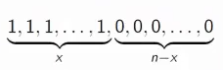
\includegraphics[width=0.3\linewidth]{figures/binom_1.png}
    \end{figure}

    Como os ensaios são independentes, temos que:

    \begin{figure}
        \centering
        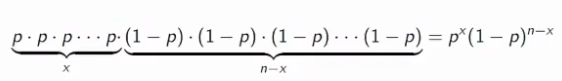
\includegraphics[width=0.5\linewidth]{figures/binom_2.png}
    \end{figure}
\end{frame}

\begin{frame}{Distribuição Binomial}
    Porém, o evento "$x$ sucessos em $n$ ensaios" pode ocorrer de diferentes ordens distintas, todas com a mesma probabilidade. 

    Como o número de ordens é o número de combinações de $n$ elementos escolhendo $x$, então a probabilidade de ocorrerem $x$ sucessos em $n$ ensaios de Bernoulli é representada por:
    $$\mathds{P}(X=x) = \binom{n}{x}p^x(1-p)^{n-x}, x = 0,1, \dots, n$$
\end{frame}

\begin{frame}{Distribuição Binomial: Exemplo}

Retira-se 3 cartas com reposição. Seja $X$ o número de vezes que sai alguma carta de copas. Ent\~ao $X\sim\mBin(3,1/4)$. 
\medskip

$\Omega_X = \{0, 1, 2, 3\}$\\
\medskip


$$\mathds{P}(X=2)={\color{blue}3}\left(\frac{1}{4}\right)^{{\color{red}2}}\left(\frac{3}{4}\right)^{\color{green}1}$$

\begin{itemize}
\item {\color{blue}3} : Número de formas de ter 2 cartas de copas em 3 tentativas\\
\item {\color{red}2} : Número de copas nas 3 tentativas\\
\item {\color{green}1} : Número de não-copas nas 3 tentativas\\
\end{itemize}
\begin{itemize}
    \item Calcule $\mathds{P}(X=0)$
\end{itemize}
\end{frame}

\begin{frame}{Distribuição Binomial}
    \textbf{Valor Esperado e Variância}: $\mathbb{E}[X] = np$ e $Var(X) = np(1-p)$
\end{frame}

\begin{frame}{Distribuição Binomial: Exemplo}
    Voltar ao exemplo das pastilhas. 
\end{frame}
\begin{frame}{Distribuição Binomial: Exemplo}
    \begin{exemplo}[14]
        Certo jogador de basquete costuma acertar 70\% dos lançamentos
na cesta. Esse jogador foi convidado para participar de um evento beneficente
em que ele pode arrecadar um grande prêmio para uma instituição de sua escolha se ele fizer 10 lançamentos e acertar todos. Supondo que os lançamentos
são independentes, qual a probabilidade de ele conseguir o prêmio?
    \end{exemplo}
\end{frame}

\begin{frame}{Distribuição Binomial: Exemplo}
    \begin{exemplo}[16]
        Cada amostra de ar tem uma probabilidade de 10\% de conter um determinado poluente orgânico. Considere 18 amostras que sejam independentes com relação à presença do poluente. Seja a variável aleatória $X$ definida como o número de amostras de ar que contêm o poluente orgânico. pergunta-se:

        \begin{itemize}
            \item Qual a probabilidade de que exatamente duas amostras contenham o poluente
            \item Qual a probabilidade de que pelo menos 4 amostras contenham o poluente. 
        \end{itemize}
    \end{exemplo}
\end{frame}

\begin{frame}{Distribuição de Poisson}

Seja um experimento realizado nas seguintes condições:

\begin{enumerate}
    \item As ocorrências são independentes
    \item As ocorrências são aleatórias
    \item A variável aleatória $X$ é o número de ocorrências de um evento ao longo de algum intervalo
\end{enumerate}

    Vamos definir a variável aleatória $X$como sendo o número de ocorrências em um intervalo. Portanto, $X$ poderá assumir os valores $0, 1, \dots $(sem limite superior)
\end{frame}

\begin{frame}{Distribuição de Poisson}
    Uma variável aleatória segue a distribuição de Poisson se sua função de probabilidade é dada por:

    $$\mathds{P}(X=x)=\dfrac{e^{-\lambda} \lambda^x}{x!}, \quad x=0,1,2,\dots$$

    em que o parâmetro $\lambda > 0$ representa a taxa média de ocorrência por unidade de medida(tempo,  por exemplo)
\end{frame}

\begin{frame}{Distribuição de Poisson}
    Notação: $X \sim$ Poisson($\lambda$)
    Esperança e Variância: $\mathbb{E}[X] = Var(X) = \lambda$
\end{frame}


\begin{frame}{Exemplo: Distribuição de Poisson}
    Sabe-se que em média ocorrem 2 terremotos por semana em certa
região do mundo. Numa dada semana, qual a probabilidade de ocorrerem 4
terremotos nessa região?

\end{frame}

\begin{frame}{Exemplo: Distribuição de Poisson}
    \begin{exemplo}[18]
        Chamadas telefônicas são recebidas à taxa de 48 por hora no balcão de reservas da Regional Airways

        \begin{itemize}
            \item Calcule a probabilidade de serem recebidas três chamadas em um intervalo de cinco minutos?
            \item Calcule a probabilidade de serem recebidas exatamente 10 chamadas em 15 minutos.
        \end{itemize}
    \end{exemplo}
\end{frame}


\end{frame}

\begin{frame}{Variáveis aleatórias contínuas}
    Uma variável aleatória é contínua se assume valores em qualquer intervalo dos números reais. 

    Dessa forma, não é possível atribuir probabilidades para um ponto específico, apenas para intervalos da reta. 

    \begin{definicao}
        Dize-se que $X$ é uma variável aleatória contínua, se existir uma função $f_X$, denominada função densidade de probabilidade (fdp) de $X$ que satisfaça as seguintes condições:

        \begin{enumerate}
            \item $f(x) \geq 0$ para todo x
            \item $\int_{-\infty}^{\infty} f(x) dx = 1$
        \end{enumerate}
    \end{definicao}
\end{frame}

\begin{frame}{Variáveis aleatórias contínuas}
    Exemplos de variáveis aleatórias contínuas:
    \begin{itemize}
        \item Altura de estudantes em uma disciplina
        \item Intervalo de tempo entre chegadas de um ônibus
        \item Peso de pessoas
        \item Profundidade de lagos
    \end{itemize}
\end{frame}
\begin{frame}{Variáveis aleatórias contínuas}
Nesse caso, temos:
   $$ \mathds{P}(a \leq X \leq b) = \int_{a}^{b} f_X(x) dx$$

   O que implica que
   $$\mathds{P}(X =a) = 0$$

   \begin{figure}
       \centering
       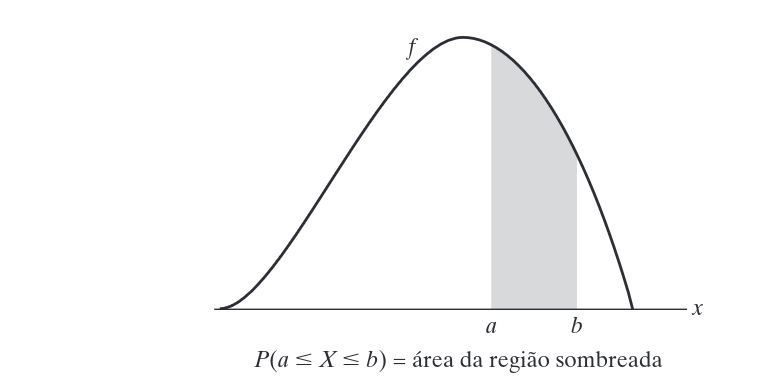
\includegraphics[width=0.7\linewidth]{figures/continua_1.png}
   \end{figure}
\end{frame}

\begin{frame}{Variáveis aleatórias contínuas}
    \begin{exemplo}[20]
        Suponhamos que um ponto seja escolhido no intervalo $(0,1)$.Representemos por $X$ a variável aleatória cujo valor seja a abcissa $x$ do ponto escolhido. 

        Seja $I \subset$ $(0,1)$, etão $\mathds{P}(X \in I)$ será diretamente proporcional ao comprimento de $I$.

        Qual é a fdp de $X$? Podemos encontrar uma função $f$ tal que:
        \pause
        $$\mathds{P}(a<X<b) = \int_{a}^{b} f(x) dx$$
        \pause
        Perceba que se $a<b<0$ ou $1<a<b, \mathds{P}(a<X<b) =0$ e, portanto, $f(x) =0$. Se $0<a<b<1, \mathds{P}(a<X<b) = b-a$ e, portanto, $f(x) = 1$. Dessa forma, temos que:

        $$f(x) = \begin{cases}
            1, &0<x<1\\
            0, &\text{ caso contrário}
        \end{cases}$$
    \end{exemplo}
\end{frame}

\begin{frame}{Variáveis aleatórias contínuas}
    \begin{exemplo}[21]
        Suponha que $X$ seja uma variável aleatória contínua cuja função densidade de probabilidade é dada por:

        $$f_X(x) = \begin{cases}
            C(4x -2x^2) & 0<x<2\\
            0 & \text{ caso contrário}
        \end{cases}$$
        \begin{enumerate}[a)]
            \item Qual é o valor de C?
            \item Determine $\mathds{P}(X>1)$
        \end{enumerate}
    \end{exemplo}
\end{frame}

\begin{frame}{Variáveis aleatórias contínuas}
    A quantidade de tempo, em horas, que um computador funciona sem estragar é uma variável aleatória contínua com função deinsidade de probabilidade:

    $$f(x) = \begin{cases}
        \lambda e^{-x/100} & x\geq 0\\
        0& x<0
    \end{cases}$$
    Qual a probabilidade de que:
    \begin{enumerate}[a)]
        \item O computador funcione entre 50 e 150 horas antes de estragar?
        \item Ele funcione pelo menos 100 horas?
    \end{enumerate}
\end{frame}

\begin{frame}{Função distribuição de uma variável aleatória contínua}

   Vimos que sendo $X$ uma variável aleatória discreta:
    $$F_X(x) = \mathds{P}(X \leq x)$$

    Essa definição se manterá a mesma para variáveis aleatórias contínuas, no entanto, para obter a função distribuição teremos que nos valer do uso da integral.

    \begin{definicao}
        Seja $Y$ uma variável aleatória contínua, temos que sua função distribuição acumulada é dada por:
            $$F_Y(y) = \mathds{P}(Y \leq y) = \int_{-\infty}^{y} f_Y(y)$$
    \end{definicao}

\end{frame}
\begin{frame}{Esperança de Variáveis aleatórias contínuas}
    Para variáveis aleatórias discretas, vimos que a esperança de uma variável aleatória discreta $X$ é dada por:
    $$\mathbb{E}[X] = \sum_{x \in \Omega_X} x \mathds{P}(X=x)$$

    De forma análoga, sendo $X$ uma variável aleatória contínua, temos que:

    $$\mathbb{E}[X] = \int_{-\infty}^{\infty} x f_X(x)$$
\end{frame}
\begin{frame}{Variância de Variáveis aleatórias contínuas}
    A seguinte relação ainda é valida para variáveis aleatórias contínuas:

    $$Var(X) = \mathbb{E}[X^2] - \mathbb{E}[X]^2$$

    onde:

    $$\mathbb{E}[X^2] = \int_{-\infty}^{\infty} x^2 f_X(x)dx$$
\end{frame}

\begin{frame}{Distribuição Normal padrão}
    Uma variável aleatória $Z$ tem distribuição \textbf{Normal padrão}, se:

    \begin{itemize}
        \item $Z$ assume valores em $\mathbb{R}$
        \item A f.d.p $f_Z$ é dada por:
        $$f_Z(z) = \dfrac{1}{\sqrt{2\pi}} e^{-z^2/2}, z\in \mathbb{R}$$
    \end{itemize}

    Notação $Z \sim N(0,1)$
\end{frame}

\begin{frame}{Distribuição Normal padrão}
    Se $Z \sim N(0,1)$, $f_Z$ é simétrica em torno de 0
    $$f_Z(z) = f_Z(-z) \forall z \in \mathbb{R}$$

    Como a Normal padrão é uma distribuição contínua, a seguinte relação é valida:

    $$\mathds{P}(Z \leq z_0) = \int_{-\infty}^{z_0}\dfrac{1}{\sqrt{2\pi}} e^{-x^2/2}, \text{ para } z\in \mathbb{R}$$

    \begin{figure}
        \centering
        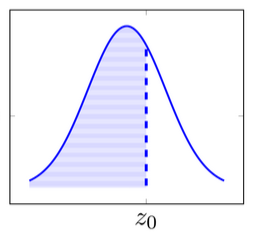
\includegraphics[width=0.3\linewidth]{figures/normal_p_1.png}
    \end{figure}

    Essa integral é impossível de ser resolvida analiticamente, nesse sentido, surge a necessidade de utilização de uma tabela.
\end{frame}

\begin{frame}{Utilizando a tabela da Distribuição Normal padrão}
    Conforme visto no slide anterior, temos que utilizar tabelas. Algumas informações importantes:

    \begin{itemize}
        \item A Normal não é a única distribuição na qual é preciso utilizar tabelas.
        \item Não existe apenas uma tabela da distribuição Normal, assim como veremos nessa aula. 
    \end{itemize}
\end{frame}

\begin{frame}{Distribuição Normal padrão}
Seja $Z \sim N(0,1)$, calcule as seguintes probabilidades:

\begin{itemize}
    \item $\mathds{P}(Z > 0)$
    \item $\mathds{P}(Z < 0)$
    \item $\mathds{P}(Z \leq 0,76)$
     \item$ \mathds{P}(Z \geq 0,76)$
     \item$ \mathds{P}(Z \leq 1,79)$
     \item$ \mathds{P}(Z \geq 2,54)$
     \item$ \mathds{P}(Z > -0,5)$
     \item$ \mathds{P}(Z < -0,5)$
     \item$ \mathds{P}(Z < -1,43)$
\end{itemize}
    
\end{frame}

\begin{frame}{Distribuição Normal($\mu, \sigma$)}
    Uma variável aleatória tem distribuição Normal com parâmetros $\mu, \sigma^2$, se:

    \begin{itemize}
        \item X assume valores em $\mathbb{R}$
        \item A f.d.p $f_X$ é dada por:

        $$f_X(x) =\dfrac{1}{\sqrt{2\pi\sigma^2}} e^{-\dfrac{(x-\mu)^2}{2\sigma^2}}, x \in \mathbb{R}$$
    \end{itemize}

    \textbf{Notação:} $X \sim N(\mu, \sigma^2)$
\end{frame}

\begin{frame}{Distribuição Normal($\mu, \sigma$)}


\textbf{Problema:} 

\begin{itemize}
\item Novamente temos uma função a qual não é possível calcular a integral analiticamente. 
    \item Só temos uma tabela para calcular propriedades envolvendo a distribuição Normal e ela considera apenas distribuições normais com média 0 e variância 1, o que fazer?
\end{itemize}
\pause
\textbf{Solução:}
    Se $X \sim N(\mu, \sigma^2)$ então:

    $$\dfrac{X - \mu}{\sigma} \sim N(0,1)$$
\end{frame}

\begin{frame}{Distribuição Normal($\mu, \sigma$)}

Considere $X \sim N(10, 5)$
    \textbf{Exemplos:}
    \begin{enumerate}[a)]
        \item $\mathds{P}(X \leq 13)$
        \item $\mathds{P}(X \geq 11,7)$
        \item $\mathds{P}(X > 9.75)$
        \item $\mathds{P}(X < 7.3)$
        \item $\mathds{P}(9,75 <X < 11,7)$
        \item $\mathds{P}(X < 9,75| X < 11,7)$
        \item O valor de c tal que $\mathds{P}(X > c) = 0.95$
    \end{enumerate}
\end{frame}

\begin{frame}{Distribuição Normal($\mu, \sigma$)}
    \begin{figure}
        \centering
        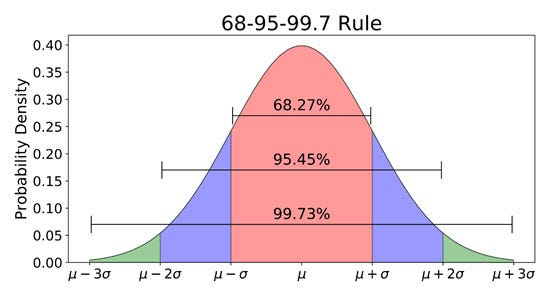
\includegraphics[width=0.8\linewidth]{figures/normal_dp.jpg}
    \end{figure}
\end{frame}
% \begin{frame}{Distribuição exponencial}
%     A distribuição exponencial é usada frequentemente para modelar o tempo decorrido entre eventos. 

%     \begin{definicao}
%         Uma variável aleatória $X$ segue a distribuição exponencial com parâmetro $\lambda>0$ se sua p.d.f é dada por:

%         $$f_X(x) = \begin{cases}
%             \lambda e^{-\lambda x}, & x>0\\
%             0, & \text{caso contrário}
%         \end{cases}$$
%     \end{definicao}
%     \textbf{Notação:}  $X \sim Exponencial(\lambda)$
% \end{frame}

% \begin{frame}{Distribuição exponencial}
% \begin{itemize}
%     \item \textbf{Média:}$\dfrac{1}{\lambda}$
%     \item \textbf{Variância:}$\dfrac{1}{\lambda^2}$
%     \item \textbf{Função distribuição acumulada:}$F_X(x) = 1 - e^{-\lambda \cdot x}$
% \end{itemize}
      
% \end{frame}

% \begin{frame}{Distribuição exponencial}

% \begin{exemplo}[22]
%     Suponha que a duração de um telefonema, em minutos, seja uma variável aleatória exponencial com parâmetro $\lambda = 1/10$. Se alguém chega logo na sua frente
% em uma cabine telefônica, determine a probabilidade de que você tenha que
% esperar:

% \begin{enumerate}[a)]
%     \item Mais de 10 minutos
%     \item Entre 10 e 20 minutos
% \end{enumerate}
% \end{exemplo}
    
% \end{frame}

% \begin{frame}{Distribuição exponencial}
%     \begin{exemplo}
%         Suponha que o número de quilômetros que um carro pode rodar sem que
% sua bateria se descarregue seja exponencialmente distribuído com um valor
% médio de 10.000 km. Se uma pessoa deseja fazer uma viagem de 5000 km,
% qual é a probabilidade de que ele ou ela consiga completar a viagem sem ter
% que trocar a bateria do carro? 
%     \end{exemplo}
% \end{frame}


% \begin{frame}{Distribuição exponencial}
%     \textbf{Perda de memória da distribuição exponencial:}

%     Seja $X$ uma variável aleatória, tal que $X\sim Exponencial(\lambda)$, mostre que: 
%     $$\mathds{P}(X \geq s+t|X \geq s ) = \mathds{P}(X \geq t)$$
% \end{frame}

% \section{Inferência Estatística}

% \begin{frame}{Inferência Estatística}

% A partir de agora mudaremos o foco do nosso curso para estudar a área da estatística conhecida como Inferência Estatística. 

% A Inferência Estatística é um conjunto de técnicas que objetiva estudar a
% população através de evidências fornecidas por uma amostra. É a amostra que
% contém os elementos que podem ser observados e, a partir daí, quantidades de
% interesse podem ser medidas.
    
% \end{frame}
% \begin{frame}{Amostragem}
%     \begin{figure}
%         \centering
%         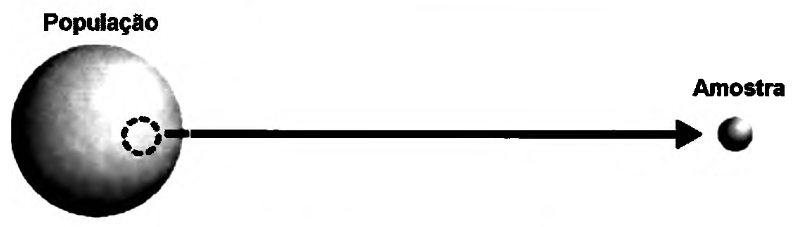
\includegraphics[width=0.5\linewidth]{figures/pop_amostra.png}
%     \end{figure}
% \end{frame}

% \begin{frame}{População}
%     \begin{definicao}
%         Dizemos que uma população é uma coleção completa de todos os elementos (valores, pessoas, medidas, etc) a serem estudados
%     \end{definicao}
% \end{frame}

% \begin{frame}{Amostra}
%     \begin{definicao}
%         Dizemos que uma amostra é um subconjunto finito da população
%     \end{definicao}
% \end{frame}

% \begin{frame}{Amostra}
%     Imagine o seguinte problema: Você deseja saber a média de reprovações de alunos em disciplinas de toda a UFRJ, no entanto, você precisa saber isso em um período de 12 horas. 

%     Nesse cenário, vários problemas podem surgir:

%     \begin{itemize}
%         \item Alguns professores podem não dar aula no dia em que a pesquisa é feita.
%         \item Talvez você não tenha tempo de se deslocar em todas as unidades da faculdade.
%         \item Alguns professores podem se recusar em te dar essa informação. 
%     \end{itemize}
% \end{frame}

% \begin{frame}{Amostra}
%     Alguns problemas permanecem em aberto:

%     \begin{itemize}
%         \item De que forma eu vou selecionar essa amostra?
%         \item Qual o tamanho da amostra que devo selecionar?
%         \item Quais garantias teóricas eu tenho de que a característica encontrada para a minha amostra realmente reflete a característica da população?
%     \end{itemize}
% \end{frame}

% \begin{frame}{Amostragem probabilística x Amostragem não-probabilística}
% \begin{itemize}
%     \item  A amostragem será probabilística se todos os elementos da população tiverem probabilidade conhecida, e diferente de zero, de pertencer à amostra. Caso contrário, a amostragem será não-probabilística.
%     \pause 
%     \item A utilização de uma amostragem probabilística é a melhor recomendação que se deve fazer no sentido de se
% garantir a representatividade da amostra, pois o acaso será o único responsável por eventuais discrepâncias entre
% população e amostra, o que é levado em consideração pelos métodos de análise da Estatística Indutiva (ou Inferência
% Estatística)
% \end{itemize}
   
% \pause
    
% \end{frame}

% \begin{frame}{Amostragem aleatória simples}
%     Amostragem aleatória simples é dos métodos de amostragem mais comumente utilizados na prática. 

%     \pause

%     \begin{definicao}
%         Uma amostra aleatória simples de tamanho $n$ de uma população de tamanho $N$ é uma amostra selecionada de forma independente e sem reposição de tal maneira que cada elemento na amostra tenha a mesma probabilidade de ser escolhido. 
%     \end{definicao}

%     \pause

%     Na prática, a amostragem simples ao acaso pode ser realizada numerando-se a população de 1 a N, sorteando-se, a
% seguir, por meio de um dispositivo aleatório qualquer, n números dessa sequência, os quais corresponderão aos
% elementos sorteados para a amostra.
% \end{frame}

% \begin{frame}{Amostragem aleatória simples}
%     \textbf{Vantagens:}
%     \begin{itemize}
%         \item Simplicidade e facilidade de execução: O processo é fácil de entender e implementar, pois basta sortear aleatoriamente os elementos sem necessidade de subdivisões ou cálculos complexos.
%         \item Garantia de resultados teóricos: Todos os principais resultados que veremos ao longo do curso tomam como base a aodção desse método de amostragem. 
%     \end{itemize}
%     \textbf{Desvantagens:}
%     \begin{itemize}
%         \item Dificuldade de aplicação em grandes populações: Para populações muito grandes, pode ser difícil enumerar todos os elementos e realizar o sorteio, tornando o processo impraticável.
%         \item Menor controle sobre a representatividade de subgrupos: Como a seleção é inteiramente aleatória, alguns subgrupos importantes da população podem acabar sendo sub-representados na amostra, especialmente em amostras pequenas.
%     \end{itemize}
% \end{frame}
% \begin{frame}{Amostragem sistemática}

%     \begin{definicao}
%         A amostragem sistemática é um tipo de amostragem probabilística, onde se faz uma seleção aleatória do primeiro elemento para a amostra e logo se selecionam os itens subsequentes utilizando intervalos fixos ou sistemáticos até chegar ao tamanho da amostra desejada.
%     \end{definicao}

%     \pause

%     \begin{exemplo}
%         Para entrevistar moradores de uma rua com 200 casas, se for preciso entrevistar 20 pessoas, divide-se o total de casas pelo número de amostras (200/20 = 10). Escolhe-se uma casa de partida aleatoriamente e, a partir daí, visita-se cada 10ª casa.
%     \end{exemplo}
    
% \end{frame}

% \begin{frame}{Amostragem sistemática}
%     A partir de sua definição, já conseguimos perceber as principais vantagens e desvantagens desse método:
%     \
    
%     \textbf{Vantagens:}
%     \begin{itemize}
%         \item Método simples e oferece um procedimento bem organizado e bem definido. 
%     \end{itemize}
    
%     \textbf{Desvantagens:}
%     \begin{itemize}
%         \item Se a amostra apresentar algum tipo de ordenação, pode acabar ocorrendo do intervalo definido acabar coincidindo com a ordenação
%         \item A única parte probabilística desse método está em escolher o primeiro item. 
%     \end{itemize}
% \end{frame}

% \begin{frame}{Amostragem por conglomerados}

%     \begin{definicao}
%         A amostragem por conglomerados é um método em que a população é dividida em grupos (ou conglomerados), que devem ser representativos e heterogêneos, ou seja, similares à população total. Em vez de selecionar elementos individuais de toda a população, alguns conglomerados são sorteados aleatoriamente, e todos os elementos dentro dos conglomerados escolhidos são incluídos na amostra. Esse método é muito usado quando a população é extensa ou dispersa geograficamente.
%     \end{definicao}

%     \begin{exemplo}
%         Para estudar o desempenho dos alunos em um estado, pode-se dividir a população em conglomerados por escola. Em vez de selecionar alunos aleatoriamente de todas as escolas, escolhem-se algumas escolas ao acaso e, em seguida, todos os alunos dessas escolas participam da amostra.
%     \end{exemplo}
% \end{frame}


% \begin{frame}{Amostragem por conglomerados}
%     \textbf{Vantagens:}
%     \begin{itemize}
%         \item Economia de tempo e custo: Como a coleta de dados é feita em grupos específicos, reduz-se a necessidade de deslocamento e logística, especialmente em áreas geográficas grandes.

% \item Amostra adequada para populações grandes e dispersas: Esse método é ideal para populações que estão espalhadas, onde é caro e impraticável acessar indivíduos dispersos.

%     \end{itemize}

%     \textbf{Desvantagens:}

% \begin{itemize}
%     \item Risco de vieses e menor precisão: Se os conglomerados não forem representativos da população, a amostra pode introduzir vieses, e a precisão pode ser menor em comparação com amostras totalmente aleatórias.

% \item Dificuldade na definição dos conglomerados: Os conglomerados precisam ser representativos da população como um todo; se forem homogêneos entre si, a amostra pode não representar bem a população total.


% \end{itemize}
% \end{frame}

% \begin{frame}{Amostragem estratificada}
%     \begin{definicao}
%         A amostragem estratificada é um método em que a população é dividida em subgrupos (ou estratos) que compartilham características comuns (como idade, renda, localização, etc.). Após a divisão, realiza-se uma amostragem aleatória em cada estrato para garantir que todos os subgrupos estejam proporcionalmente representados na amostra final. Esse método é ideal quando se quer garantir que todos os segmentos de uma população estejam incluídos na amostra.
%     \end{definicao}
% \pause
%     \begin{exemplo}
%         Na UFRJ, poderíamos realizar uma pesquisa com alunos de diferentes cursos, nesse caso os estratos seriam cada um dos cursos da UFRJ. Em seguida selecionamos aleatoriamente alunos de cada um dos cursos. Isso garante que cada curso seja representado na amostra.
%     \end{exemplo}
% \end{frame}

% \begin{frame}{Amostragem estratificada}
%     \textbf{Vantagens:}
%     \begin{itemize}
%         \item Alta representatividade: Ao incluir todos os subgrupos, a amostragem estratificada oferece uma amostra mais representativa, reduzindo o risco de vieses.

% \item Maior precisão nas estimativas: Como cada estrato é amostrado proporcionalmente, as estimativas tendem a ser mais precisas, especialmente se os estratos tiverem características distintas.
%     \end{itemize}
% \textbf{Desvantagens:}

% \begin{itemize}
%     \item Necessidade de informações detalhadas: É preciso ter informações suficientes para dividir a população corretamente nos estratos, o que nem sempre é viável ou fácil.

% \item Dificuldade de definir os estratos corretamente: Se os estratos não forem bem definidos ou não refletirem as diferenças da população, a amostra pode perder representatividade.
% \end{itemize}
% \end{frame}

% \begin{frame}{Amostragem}
%     Na prática, o método de amostragem adotado é a amostragem aleatória simples, justamente por ela possuir garantias teóricas que veremos a seguir. 
% \end{frame}


% \begin{frame}{Parâmetro x Estatística}
% \textbf{Parâmetro}
% \begin{definicao}
%     É uma medida numérica desconhecida que descreve alguma característica da população
% \end{definicao}


% \textbf{Exemplos:}
% \begin{itemize}
%     \item Média populacional ($\mu$)
%     \item Variância populacional ($\sigma^2$)
%     \item Desvio padrão populacional ($\sigma$)
%     \item Proporção populacional($\pi$)
% \end{itemize}
% \end{frame}

% \begin{frame}{Parâmetro x Estatística}
% \textbf{Estatística}
% \begin{definicao}
%     É uma medida numérica  que descreve alguma característica da amostra.
% \end{definicao}


% \textbf{Exemplos:}
% \begin{itemize}
%     \item Média amostral ($\hat{\mu}$)
%     \item Variância amostral ($\hat{\sigma}^2$)
%     \item Desvio padrão amostral ($\hat{\sigma}$)
%     \item Proporção amostral($\hat{\pi}$)
% \end{itemize}
% \end{frame}

% \begin{frame}{Primeira garantia: A média das médias amostrais é igual a verdadeira média}

%     Vamos retomar o exemplo anterior em que desejávamos realizar uma pesquisa com os professores da UFRJ para saber a média de reprovação de alunos em apenas 12 horas. 

% \pause 
% \begin{itemize}
%     \item A UFRJ conta atualmente com o total de 176 cursos.
%     \item Vamos supor que cada curso tem aproximadamente 40 disciplinas em sua grade curricular. 
%     \item Nesse caso temos aproximadamente $176 \times 40 = 7040$ professores a serem entrevistados
%     \pause
%     \item Obviamente, conforme já vimos, não será possível entrevistar todos os professores, nesse caso selecionamos uma amostra de 100 professores por meio da amostragem aleatória simples.
%     \item Esse tamanho de amostra é representativo?
% \end{itemize}
    
% \end{frame}

\begin{frame}{Relembrando a Amostragem Aleatória Simples}
 Exercício: Explique como funciona a Amostragem Aleatória Simples.
\end{frame}

\begin{frame}{Exemplo no R}
    Exemplo no R: Trabalho da Eduarda e da Larissa
\end{frame}

\begin{frame}{Distribuições amostrais}
    No exemplo do trabalho da Larissa e Eduarda, vimos que:
    \begin{itemize}
        \item A média amostral parece convergir para a média populacional a medida que $n$ aumentam
        \pause
        \item A variãncia das médias parece convergir para 0 a medida que $n$ aumenta. 
        \pause
        \item A média das médias parece ser igual a verdadeira média a media que o número de amostras aumenta.
        \pause
        \item A distribuição das médias parece ser Normal. 
    \end{itemize} 
    \pause
    Isso é sempre verdade? \pause De fato é verdade e o que nos garante isso são os dois resultados mais importantes da teoria das probabilidades,
     a Lei dos Grandes Números e o Teorema Central do Limite
\end{frame}

\begin{frame}{Lei dos Grandes Números}
A Lei dos Grandes Números possui duas versões (Na verdade mais de duas):

\pause
\textbf{Lei Fraca dos Grandes Números:}

Seja \( X_1, X_2, \dots, X_n \) uma sequência de variáveis aleatórias independentes e identicamente distribuídas (i.i.d.) com esperança \( \mu = \mathbb{E}[X_i] \) e variância finita \( \sigma^2 = \mathrm{Var}(X_i) < \infty \). Então, para todo \( \varepsilon > 0 \),
\[
\lim_{n \to \infty} \mathbb{P}\left( \left| \frac{1}{n} \sum_{i=1}^{n} X_i - \mu \right| > \varepsilon \right) = 0.
\]
\pause
\textbf{Lei Forte dos Grandes Números:}

Seja \( X_1, X_2, \dots, X_n \) uma sequência de variáveis aleatórias independentes e identicamente distribuídas (i.i.d.) com esperança \( \mu = \mathbb{E}[X_i] \). Suponha que \( \mathbb{E}[|X_i|] < \infty \). Então,
\[
\frac{1}{n} \sum_{i=1}^{n} X_i \xrightarrow{\text{quase certamente}} \mu, \quad \text{isto é,} \quad \mathbb{P}\left( \lim_{n \to \infty} \frac{1}{n} \sum_{i=1}^{n} X_i = \mu \right) = 1.
\]

\end{frame}

\begin{frame}{Teorema Central do Limite}

    Se $n$  for suficientemente grande, então $\Bar{X}$ terá uma distribuição aproximadamente Normal de média $\mu$ e variância $\sigma^2/n$, ou seja:

    $$\Bar{X} = \dfrac{1}{n}\sum_{i=1}^n X_i \sim N\left( \mu, \dfrac{\sigma^2}{n}\right)$$
\end{frame}

\begin{frame}{Primeira garantia: A média das médias amostrais é igual a verdadeira média}

    Por meio do Teorema Central do Limite, temos o seguinte resultado:

    $$\mathbb{E}[\Bar{X}] = \mu $$
\end{frame}

\begin{frame}{Segunda garantia: A variância da média amostral}

    Além disso, temos também garantias sobre a variância:
    $$Var(\Bar{X}) = \dfrac{\sigma^2}{n}$$

   \pause

   Perceba que quando $n\to \infty$, $\dfrac{\sigma^2}{n} \to 0$
\end{frame}

\begin{frame}{Teorema Central do Limite}
    Outra forma de ver o \textbf{Teorema Central do Limite} é o padronizando:

     Seja $X_1, X_2, \dots, X_n$ uma sequência de variáveis aleatórias independentes e identicamente distribuídas com média $\mu$ e variância $\sigma^2$, então:

    $$\dfrac{\Bar{X} - \mathbb{E}[\Bar{X}]}{\sqrt{Var(\Bar{X}})} = \dfrac{\Bar{X} - \mu}{\sqrt{\dfrac{\sigma^2}{n}}} \xrightarrow[n \to \infty ]{\text{em distribuição}} N(0,1)$$

    $$\dfrac{\sum_{i=1}^n X_i - n\mu}{\sqrt{n\sigma^2}}  \xrightarrow[n \to \infty ]{\text{em distribuição}} N(0,1)$$
    \pause
    Uma pergunta que fica é: Na prática, qual $n$ é considerado suficientemente grande?
\end{frame}


\begin{frame}{Estimação por intervalo}

\begin{itemize}
    \item Até agora só vimos os estimadores pontuais, que fornecem como estimativa um único valor numérico para o parâmetro de interesse. 
    \item  O método de estimação por intervalo visa estabelecer um intervalo de confiança, incorpora, à estimativa pontual do parâmetro,
informações a respeito da variabilidade do estimador. Intervalos de confiança são
obtidos através da distribuição amostrai de seus estimadores.
\end{itemize}
    
\end{frame}

\begin{frame}{Intervalo de confiança}
    \begin{figure}
        \centering
        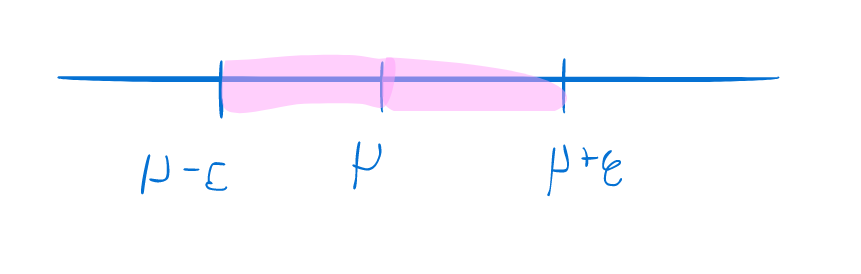
\includegraphics[width=0.8\linewidth]{figures/confidence_interval.png}
    \end{figure}
\end{frame}


\begin{frame}{Caso 1: Variância conhecida}
    Considere que temos interesse em construir um intervalo de confiança para a média $\mu$ de uma certa população com variância conhecida $\sigma^2$. Supondo uma amostra de tamanho $n$, vimos que a média amostral tem distribuição Normal com a mesma média $\mu$ e variância $\sigma^2/n$, ou seja, 

    $$Z =\dfrac{\Bar{X} - \mu}{\sigma/\sqrt{n}} \sim N(0,1)$$

    \pause

    Logo, fixando um valor $\alpha$ tal que $0<\alpha<1$, podemos encontrar dois valores $a$ e $b$ tal que:

    $$\mathds{P}(a <Z < b) = \alpha$$
\end{frame}

\begin{frame}{Caso 1: Variância conhecida}
    $$\mathds{P}(a <Z < b) = \alpha$$

    \begin{itemize}
        \item Perceba que, como a distribuição Normal é simétrica, podemos dizer que a = -b.
        \item Além disso, $a$ e $b$ são funções de $\alpha$. Qual é a regra dessa função?
    \end{itemize}
    \pause

    De fato, $a=-z_{\alpha/2}$ e $b = z_{\alpha/2}$
   
\end{frame}

\begin{frame}{Caso 1: Variância conhecida}
    $$\mathds{P}(-z_{\alpha/2} <Z < z_{\alpha/2}) = \alpha$$

    \begin{figure}
        \centering
        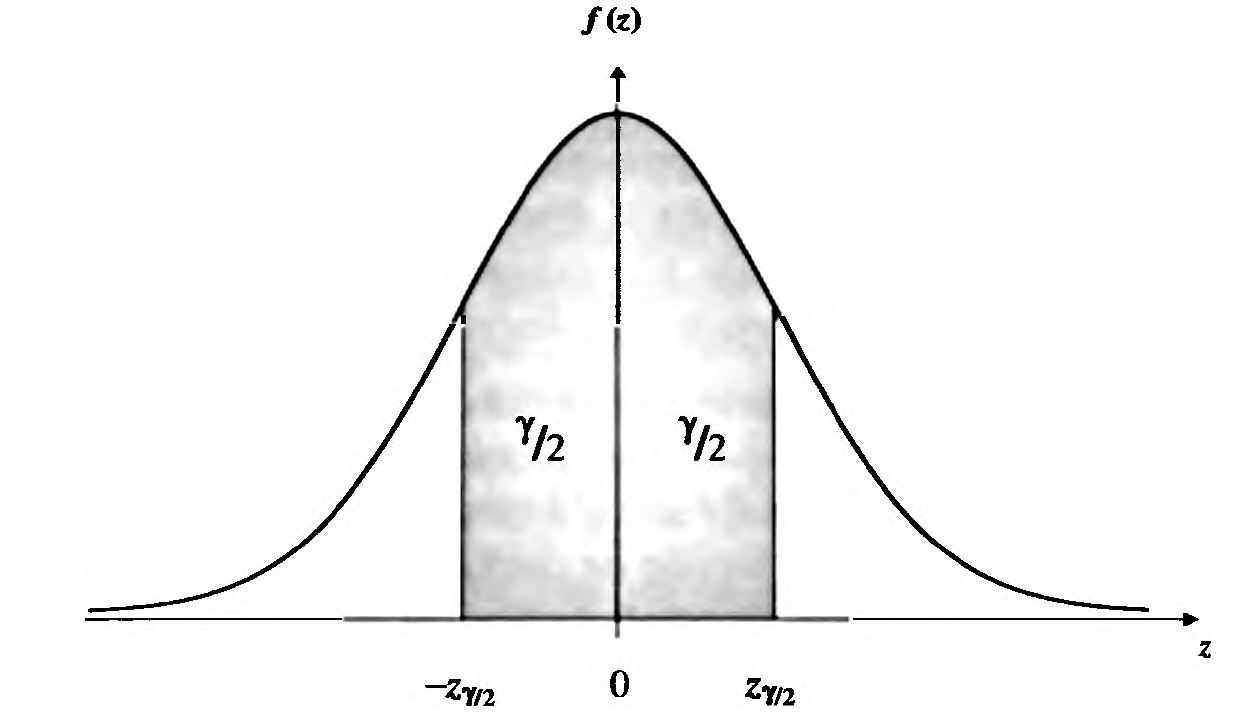
\includegraphics[width=0.6\linewidth]{figures/confidence_interval_2.png}
    \end{figure}
\end{frame}

\begin{frame}{Caso 1: Variância conhecida}
    Substituindo, temos que:

    \begin{align*}
        \mathds{P}(-z_{\alpha/2} <Z < z_{\alpha/2}) &= \mathds{P}\left(-z_{\alpha/2} < \dfrac{\Bar{X} - \mu}{\sigma/\sqrt{n}} < z_{\alpha/2}\right)\\
        &= \mathds{P}\left(\Bar{X} -z_{\alpha/2}\dfrac{\sigma}{\sqrt{n}} < \mu < \Bar{X} + z_{\alpha/2}\dfrac{\sigma}{\sqrt{n}}\right)
    \end{align*}

    Dessa forma, o intervalo de confiança para $\mu$, com coeficiente de confiança $\alpha$ é dado por:

    $$IC(\mu, \alpha) = \left[ \Bar{X} - z_{\alpha/2}\dfrac{\sigma}{\sqrt{n}} ; \Bar{X}+ z_{\alpha/2}\dfrac{\sigma}{\sqrt{n}}\right]$$

    $ z_{\alpha/2}\dfrac{\sigma}{\sqrt{n}}$ é denominada margem de erro.
\end{frame}

\begin{frame}{Caso 1: Variância conhecida}
    \textcolor{red}{Super Mega Importante} - \textbf{Interpretação do intervalo de confiança:} Se obtivermos várias
amostras de mesmo tamanho e, para cada uma delas, calcularmos os
correspondentes intervalos de confiança com coeficiente de confiança $\alpha$ ,
esperamos que a proporção de intervalos que contenham o valor de $\mu$ seja igual
a $\alpha$ .

Ou seja, se coletarmos 1000 amostras encontrarmos o intervalo de confiança para $\mu$ com nível de confiança $95\%$, então espera-se que 950 intervalos contenham a média populacional.  
\pause

\vspace{10px}

\begin{figure}
    \centering
    
\includegraphics[width=0.4\linewidth]{figures/mu_crying.jpg}
\end{figure}
\end{frame}

\begin{frame}{Caso 1: Variância conhecida}
    \begin{exemplo}
        Considere que a altura dos estudantes de uma escola siga a distribuição Normal com média $\mu$ desconhecida e variância igual a $10^{-2}$ .
         Uma amostra de dez estudantes foi sorteada e forneceu média 1,69. 
         Forneça uma estimativa para o parâmetro desconhecido $\mu$ \pause com 95\% de confiança e interprete o resultado obtido. 
         \pause Agora calcule com 99\% de confiança. \pause Agora calcule com 50\% de confiança. 
    \end{exemplo}
\end{frame}


% \begin{frame}{Caso 2: Variância desconhecida}
% Na prática é muito comum encontrarmos cenários em que não se tem a variância populacional. 

% O que fazer nesse caso?

% \pause 

% A solução é muito simples, basta substituir o desvio padrão pelo seu estimador.

% $$IC(\mu, \alpha) = \left[ \Bar{X} - t_{c}\dfrac{\hat{\sigma}}{\sqrt{n}} ; \Bar{X}+ t_{c}\dfrac{\hat{\sigma}}{\sqrt{n}}\right]$$

% No entanto, perceba que agora ao invés de $z$, temos $t$. Isso ocorre pois o teorema central do limite foi violado, mas, encontrou-se uma nova distribuição que parecia ser adequada nesse caso, a t de Student.
% \end{frame}

% \begin{frame}{Caso 2: Variância desconhecida}
%     Nesse caso, temos o seguinte resultado:

%     $$\dfrac{\Bar{X} - \mu}{\hat{\sigma}/\sqrt{n}} \sim t_{n-1}$$
% \end{frame}

% \begin{frame}{Distribuição t de Student}

% \textbf{Características da distribuição}
%     \begin{itemize}
%         \item É simétrica com média t = 0, assim como a Normnal(0,1) era.
%         \item Apresenta comportamento diferente dependendo do número de graus de liberdade
%         \item Conforme os graus de liberdade aumentam, mais próxima ela se torna da Normal
%     \end{itemize}

%     \begin{figure}
%         \centering
%         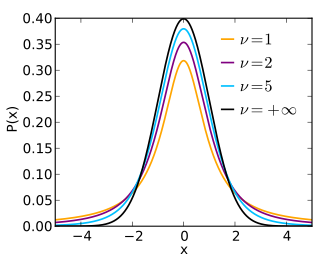
\includegraphics[width=0.5\linewidth]{figures/Student_t_pdf.svg.png}
%     \end{figure}
% \end{frame}

% \begin{frame}{Caso 2: Variância desconhecida}
%     \begin{exemplo}
%     Uma máquina que produz doces estava programada para fazer bombom com peso médio de 450g. Agora, devido a falhas mecanincas, o equipamente desregulou e, antes que ocorra um prejuizo, deseja-se saber qual o novo peso médio. Para isso, foi retirada uma amostra de 29 bombons que apresentaram média igual a 534g e desvio padrão igual a 20g. Calcule um intervalo de confiança para a média populacional considerando $95\%$ de confiança. 
%     \end{exemplo}
% \end{frame}

% \begin{frame}{Caso 2: Variância desconhecida}
%     Em uma amostra aleatória de 20 municípios do Rio de Janeiro, considerando-se os dados da Secretaria de Segurança Pública relativos ao crime de lesão corporal, a média de crimes é de 87 e o desvio padrão igual a 101,94. Construa um intervalo de 99\% de confiança para a média populacional. 
% \end{frame}
% \begin{frame}{Caso 3: Proporção}
%     Um resultado bastante útil que podemos usar em decorrência do Teorema Central do Limite é a possibilidade de aproximar uma distribuição Binomial para uma distribuição Normal. 

%     \textbf{Como fazer isso? }

%     Primeiramente, temos que lembrar que se $X \sim Binomial(n, p)$, então:

%     $$X = W_1 + W_2 + W_3 + \dots + W_n$$

%     onde $W_i \sim Bernoulli(p)$

%     Logo, pelo Teorema Central do Limite:

%     $$X \sim N(E[X], Var(X))$$

%     ou seja, 

%     \pause

%     $$X \sim N(np, np(1-p))$$
% \end{frame}


\begin{frame}{Caso 3: Proporção}
    Um estimador (estatística) natural para estimar a proporção populacional seria considerar  seria basicamente somar a quantidade dos eventos de interesse e dividr pelo total:

    $$\hat{p} = \dfrac{\sum_{i=1}^n W_i}{n}$$

    Logo, 

    $$\hat{p} \sim N\left(p, \dfrac{p(1-p)}{n}\right)$$
\end{frame}

\begin{frame}{Caso 3: Proporção}
    Dessa forma, um intervalo de confiança com nível de confiança $\alpha$ é dado da seguinte forma:

    $$IC(\pi, \alpha) = \left[ \hat{p} - z_{\alpha/2}\sqrt{\dfrac{p(1-p)}{n}} ; \hat{p}+ z_{\alpha/2}\sqrt{\dfrac{p(1-p)}{n}}\right]$$
\end{frame}

\begin{frame}{Caso 3: Proporção}
    \begin{exemplo}
        Uma empresa visa oferecer uma conta universitária para os alunos da UFRJ e gostaria de saber quantos alunos vão aceitar a oferta. A empresa decide enviar uma oferta para 1000 alunos e 140 aceitam criar a conta universitária

        \begin{enumerate}
            \item Qual o tamanho da amostra $(n)$?
            \item Qual a proporção amostral $(\hat{p})$
            \item Construa um intervalo de confiança com 5\% de significância para a proporção de alunos que irão aceitar criar a conta. 
        \end{enumerate}
    \end{exemplo}
\end{frame}

\begin{frame}{Caso 3: Proporção}
    \begin{exemplo}
         Numa pesquisa com 50 eleitores, o candidato José João obteve a preferência de
17 desses eleitores. Supondo que a eleição ocorresse na época da pesquisa,
construa os intervalos de confiança otimista e conservador (p=1/2) para a proporção de
votos a serem recebidos pelo candidato mencionado. Use um coeficiente de
confiança igual a 94\%.
    \end{exemplo}
\end{frame}

\begin{frame}{Calculando o tamanho da amostra}
    \begin{exemplo}
        Uma pesquisa eleitoral tem o objetivo de entender quantas pessoas irão votar em um determinado prefeito no ano de 2024. Ela deseja ter uma margem 
        de erro de 1\% para mais ou para menos e com nível de confiança 95\%. Com base em experiências passadas, ela espera que aproximadamente 50\% dos entrevistados irão votar no candidato.

        \pause

        Temos que:

\begin{align*}
    z_{\alpha/2}\sqrt{\dfrac{p(1-p)}{n}} &= 0,01 \implies 1,96 \cdot \sqrt{\dfrac{0,25}{n}} = 0,1\\
    & \implies \dfrac{0,25}{n} = \left(\dfrac{0,01}{1,96}\right)^2 \implies n \approx 9604 
\end{align*}
    \end{exemplo}
\end{frame}

% \begin{frame}{Testes de Hipóteses}

% \begin{itemize}
%     \item Nos teste de hipóteses, estamos interessados em saber se determinada afirmação sobre uma população, usualmente sobre um parâmetro dessa, desejamos saber se os resultados
% experimentais provenientes de uma amostra contrariam ou não tal afirmação.
%     \item O objetivo do teste estatístico de hipóteses é, então, fornecer uma metodologia que nos permita verificar se os dados amostrais trazem evidências que apoiem ou não uma hipótese (estatística) formulada.
% \end{itemize}
    
% \end{frame}

% \begin{frame}{Procedimento geral do Teste de Hipóteses}
% \begin{itemize}
%     \item A construção de um teste de hipóteses, para um parâmetro populacional, pode ser
% colocada do seguinte modo. Existe uma variável X associada a dada população e tem-se
% uma hipótese sobre determinado parâmetro $\theta$ dessa população.
% \end{itemize}
% \end{frame}

% \begin{frame}{Procedimento geral do Teste de Hipóteses}
% \begin{exemplo}
%     Supondo que a distribuição dos valores da glicemia de jejum em uma população de pessoas não diabéticas seja normal, um pesquisador deseja testar a hipótese de que a média de glicemia de jejum nessa população seja igual a 85 mg/dl. Como proceder?
% \end{exemplo}
%    \pause
% \begin{itemize}
%     \item Vamos tentar resolver esse problema utilizando o que já aprendemos de intervalos de confiança.
%     \pause
%     \item Sabemos que o intervalo de confiança para a média quando a variância é desconhecida é dada por:
% \end{itemize}

% $$IC(\mu, \alpha) = \left[ \Bar{X} - t_{\frac{\alpha}{2}, n-1}\dfrac{\hat{\sigma}}{\sqrt{n}} ; \Bar{X}+ t_{\frac{\alpha}{2}, n-1}\dfrac{\hat{\sigma}}{\sqrt{n}}\right]$$
% \end{frame}

% \begin{frame}{Procedimento geral do Teste de Hipóteses}
%     Vamos separar o procedimento do teste de hipóteses em 5 passos. 
% \textbf{Passo 1:} Expressar o tema da pesquisa em termos de uma hipótese estatística
%     \begin{itemize}
%         \item O primeiro passo para montar nosso teste de hipóteses é estabelecer uma hipótese que será avaliada. Essa hipótese é chamada de hipótese nula, representada por $H_0$. No exemplo anterior, a hipótese nula é de que a distribuição de probabilidades da glicemia de jejum na população que estamos estudando é normal com média igual a 85 mg/dl. \item Ao estabelecermos uma hipótese a ser testada, a mesma será confrontada com uma hipótese alternativa, representada por $H_1$. No exemplo acima, a hipótese alternativa é que a distribuição de probabilidades da glicemia de jejum na população que estamos estudando é normal com média diferente de 85 mg/dl.
%     \end{itemize}
% \end{frame}

% \begin{frame}{Procedimento geral do Teste de Hipóteses}
% Nesse caso temos:

%         $$\begin{cases}
%             H_0: \mu = 85 mg/dl \\
%             H_1: \mu \neq 85 mg/dl
%         \end{cases}$$
% \end{frame}
% \begin{frame}{Procedimento geral do Teste de Hipóteses}
% \textbf{Passo 2:} Selecionar o nível de confiança ($\alpha$)

% \begin{itemize}
%     \item Precisamos atribuir um nível de confiança $\alpha$ para o teste. A ideia é a mesma utilizada para o intervalo de confiança. Para esse exemplo vamos supor $\alpha=95\%$.
% \end{itemize}
    
% \end{frame}

% \begin{frame}{Procedimento geral do Teste de Hipóteses}
%     \textbf{Passo 3: Selecionar a amostra e realizar os cálculos}

%     No exemplo anterior, vamos supor que selecionamos uma amostra que apresentou os seguintes resultados:
% \begin{itemize}
%     \item $\Bar{x}$ = 92 mg/dl
%     \item n = 36
%     \item s = 16 mg/dl
% \end{itemize}
% \end{frame}

% \begin{frame}{Procedimento geral do Teste de Hipóteses}

% \textbf{Passo 4:} Tomar a decisão

% \begin{itemize}
%     \item Vamos calcular o intervalo de confiança para a média populacional
%     \pause
%     \item Nesse caso, rejeita-se a hipótese nula, pois $85$ não está presente no intervalo calculado. 
% \end{itemize}
% \end{frame}

% \begin{frame}{Procedimento geral do Teste de Hipóteses}
%     E se tivéssemos:
%     \begin{itemize}
%     \item $\Bar{x}$ = 89 mg/dl
%     \item n = 36
%     \item s = 16 mg/dl
%     \pause
%     \item Devemos aceitar a hipótese nula?
% \end{itemize}
% \end{frame}
% \end{document}


\end{document}
